\chapter{Event selection, datasets and MC samples}
    \label{sec:samples_selection}
    This chapter contains the description of the data and MC samples, used in the analysis, as well as the applied cuts. It also describes the event-level correction of the Z axis position of the primary vertex. The chapter concludes with the set of control plots of the main observables.
    \section{Data and MC samples}
     \subsection{Data samples}
    The data samples for this study were collected with special beam conditions that ensure low pile-up. The MC samples were generated to match these conditions.s The data samples were collected in three runs:
    \begin{itemize}
    \item $\sqrt{s} = 5.02\tev$ data taken in November 2017, ATLAS data
    period M, preliminary calibrated luminosity $256.827\,\ipb$ with an uncertainty
    of $\pm 1.6\%$.
    \item $\sqrt{s} = 13\tev$ data taken in November 2017, ATLAS data
    period N, preliminary online luminosity $146.6\ipb$.
    \item $\sqrt{s} = 13\tev$ data taken in June 2018, ATLAS data
    period G4+J, preliminary online luminosity $193.2\ipb$.
    \end{itemize}

	The luminosity  calibration for the 13 TeV runs is not available yet, the corresponding uncertainty is not known, but is expected to be around 3\%. The runs of November 2017 and the run of June 2018 had the same bunch spacing of 25 ns, but a different filling scheme. The two main differences from the high-$\mu$ data collection are the following:
	\begin{itemize}
	\item In order to optimize topo-cluster response for the \gls{hr} lower topo-cluster thresholds were used. 
	\item Single $e$ and $\mu$ triggers with significantly lower
	thresholds and looser identification criteria are run without
	prescale, most notably \texttt{HLT\_e15\_lhloose\_nod0\_L1EM12} and
	\texttt{HLT\_mu14}.
	\end{itemize}	

	At the beginning of 5 TeV fills the pile-up reached $\mu \sim 5$, slowly descending to $\mu \sim 1$ by the end of the run. In the case of 13 TeV the luminosity was levelled at $\mu = 2$ in the course of the run. The corresponding distributions for $\mu$ and $N_{PV}$ for the 5 TeV and 13 TeV runs are shown in Fig. \ref{fig:mu5} and Fig. \ref{fig:mu13}.
	\begin{figure}[tph]
		\centering
		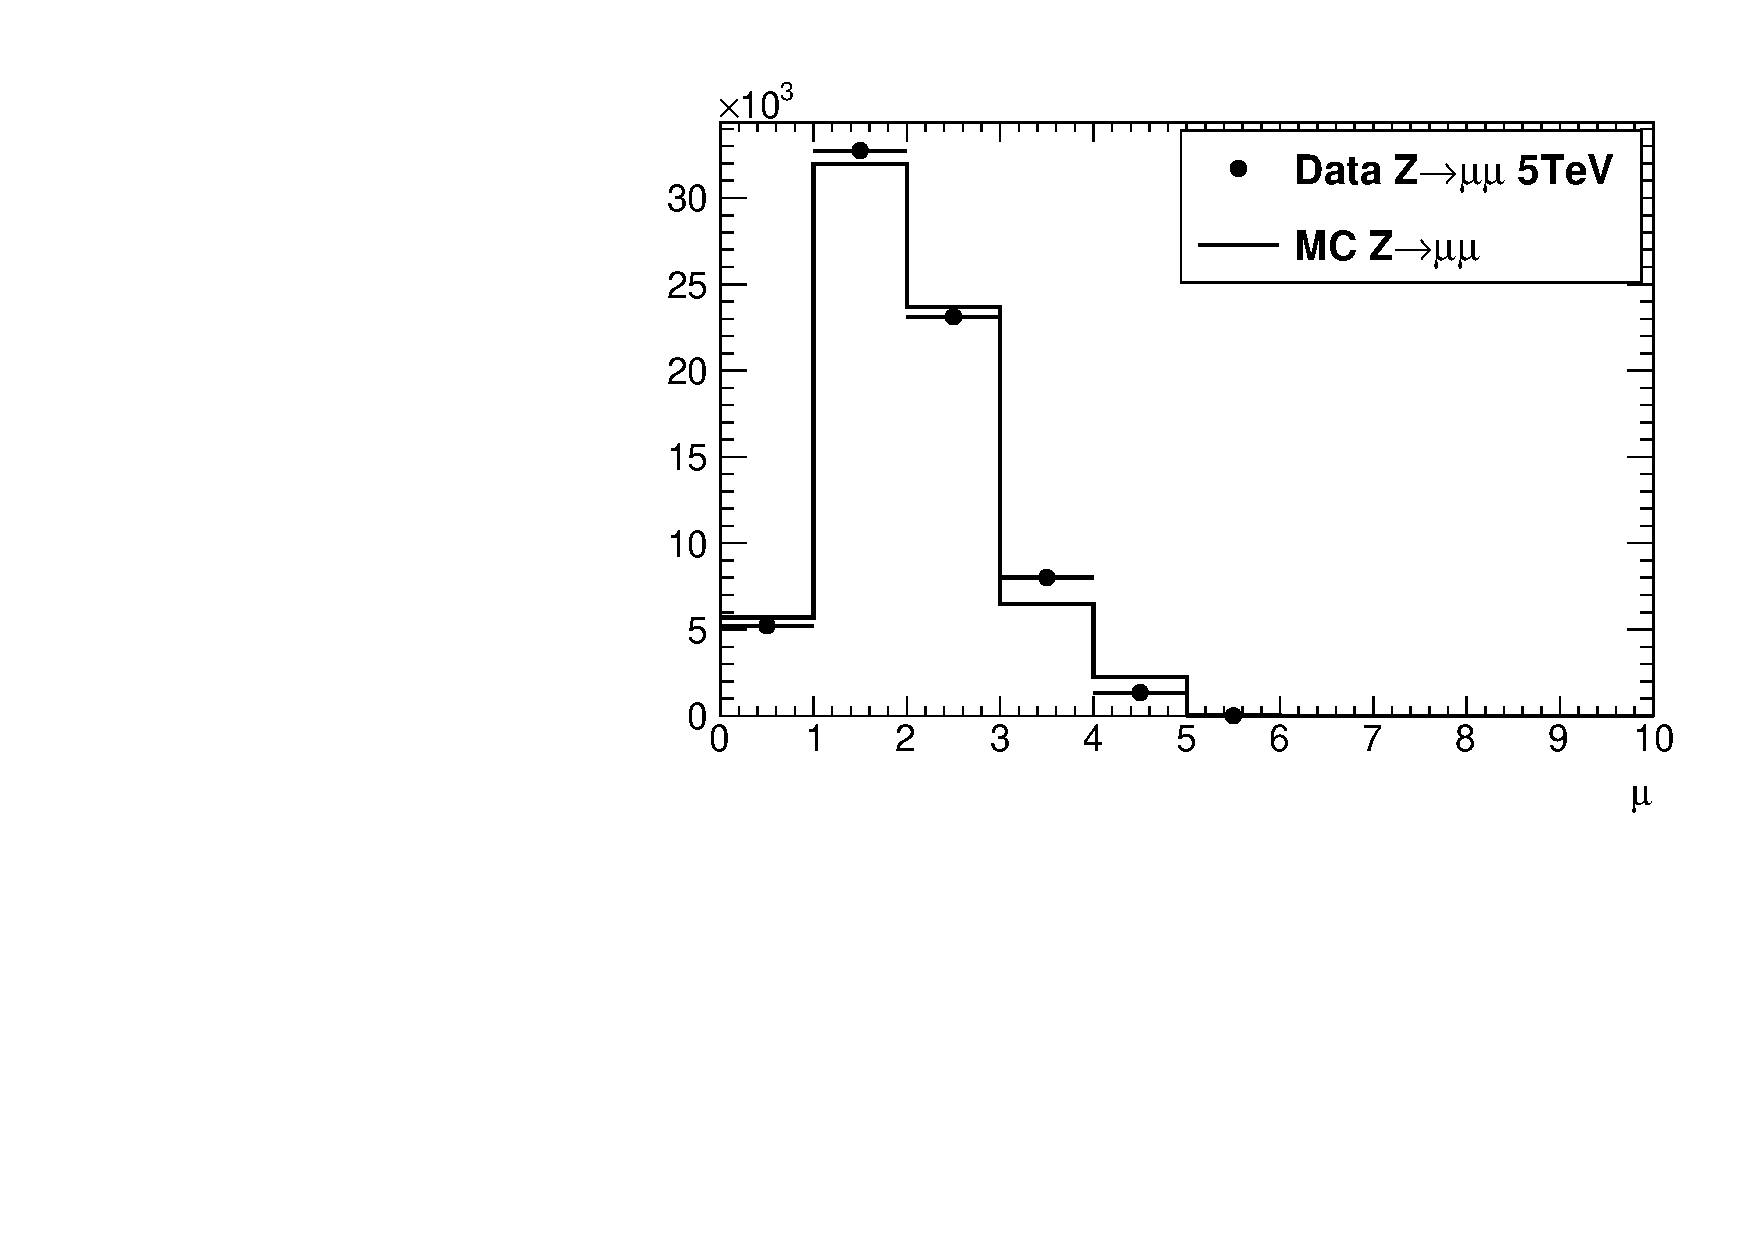
\includegraphics[width=.33\textwidth]{zmumu_5tev_mu.pdf}%
		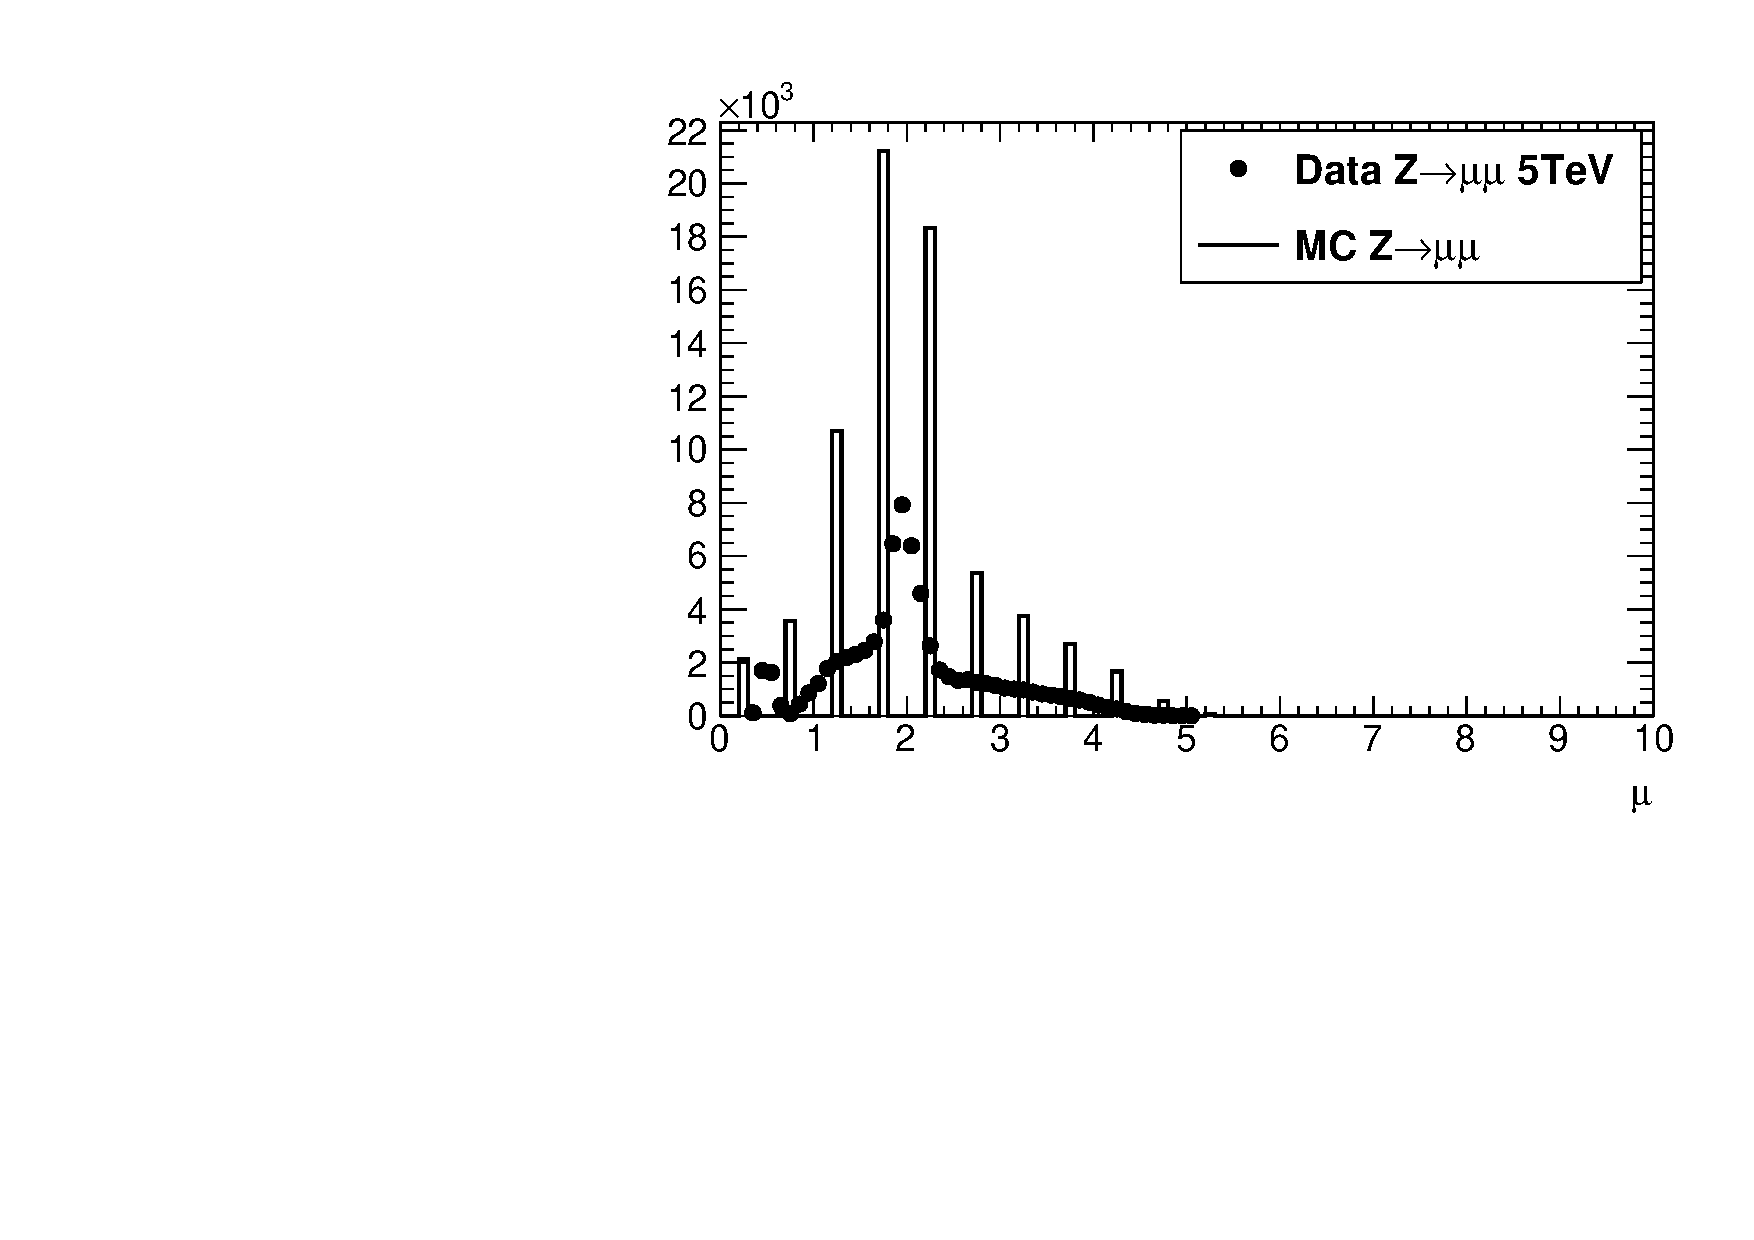
\includegraphics[width=.33\textwidth]{zmumu_5tev_mufine.pdf}%
		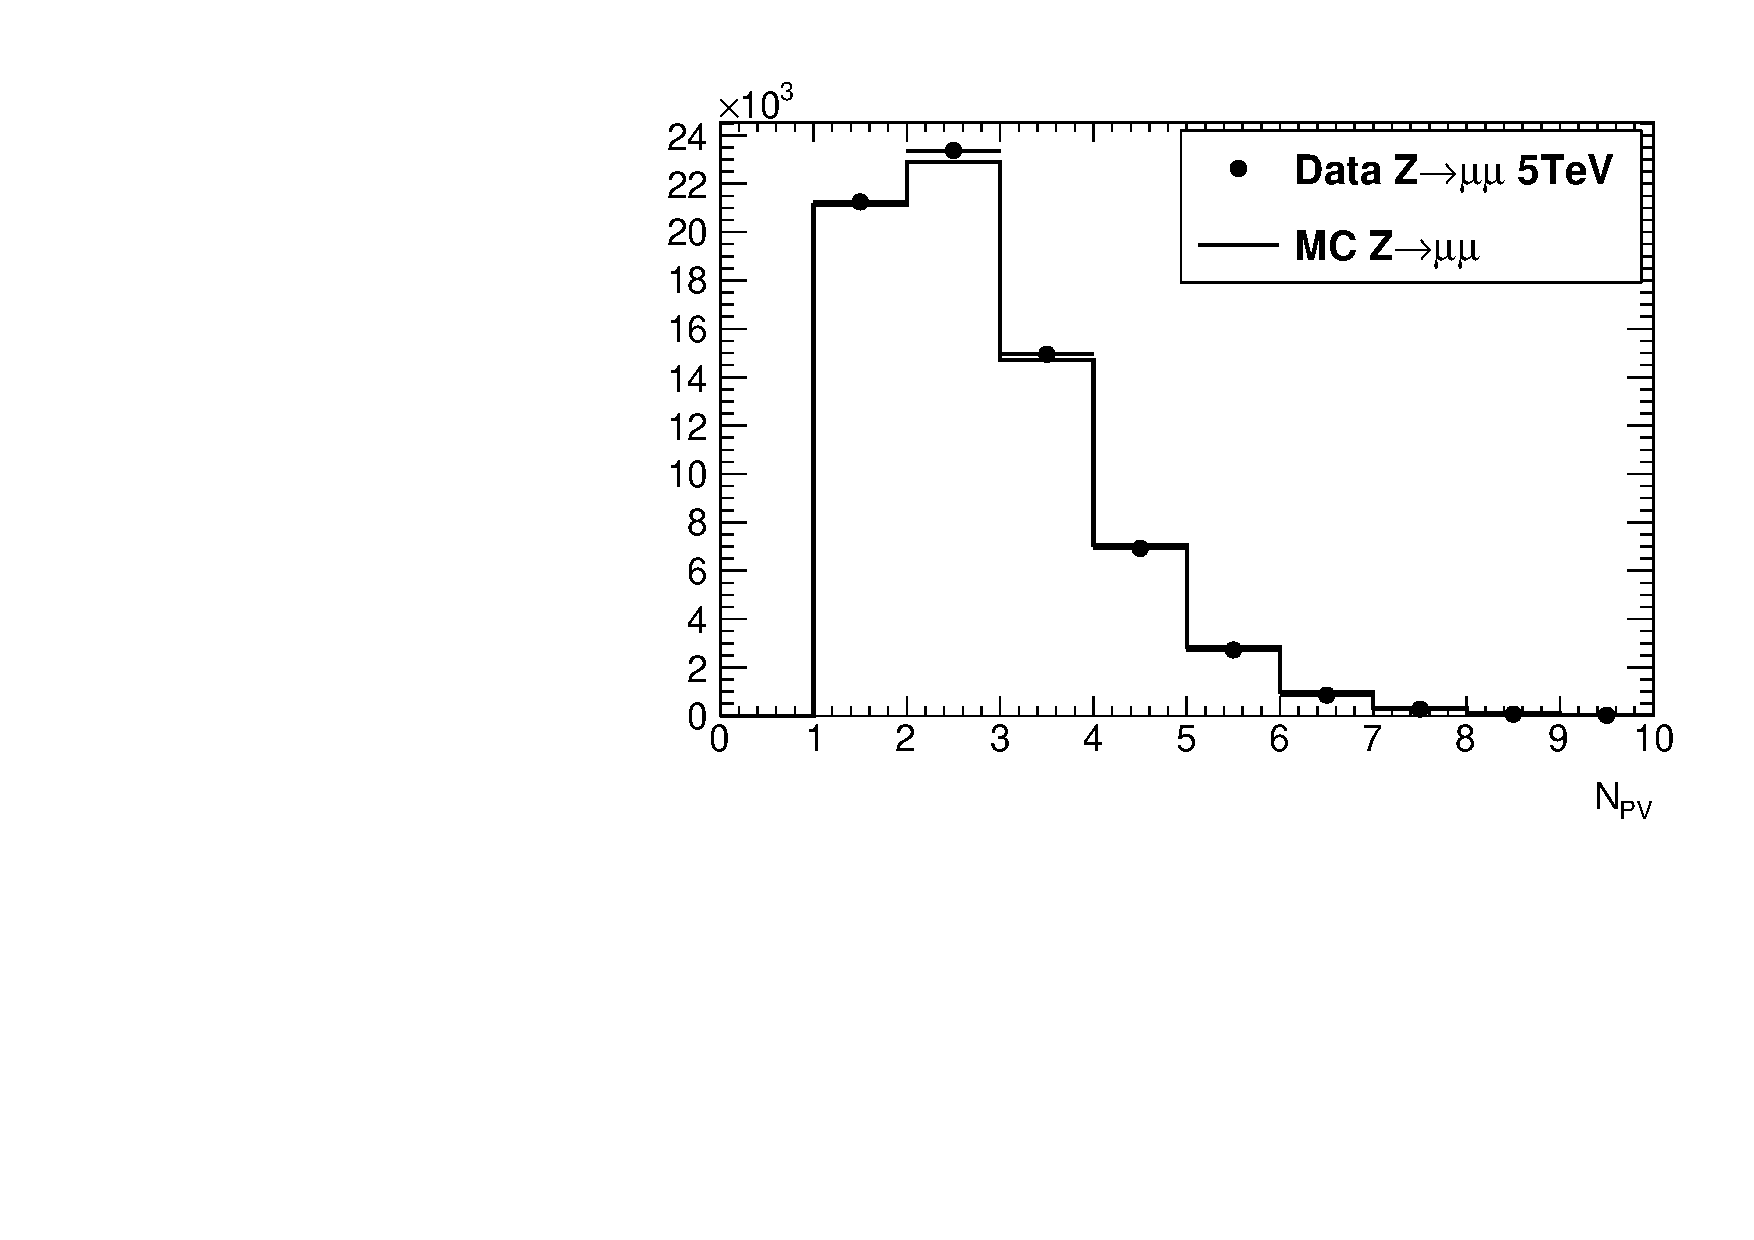
\includegraphics[width=.33\textwidth]{zmumu_5tev_npv.pdf}
		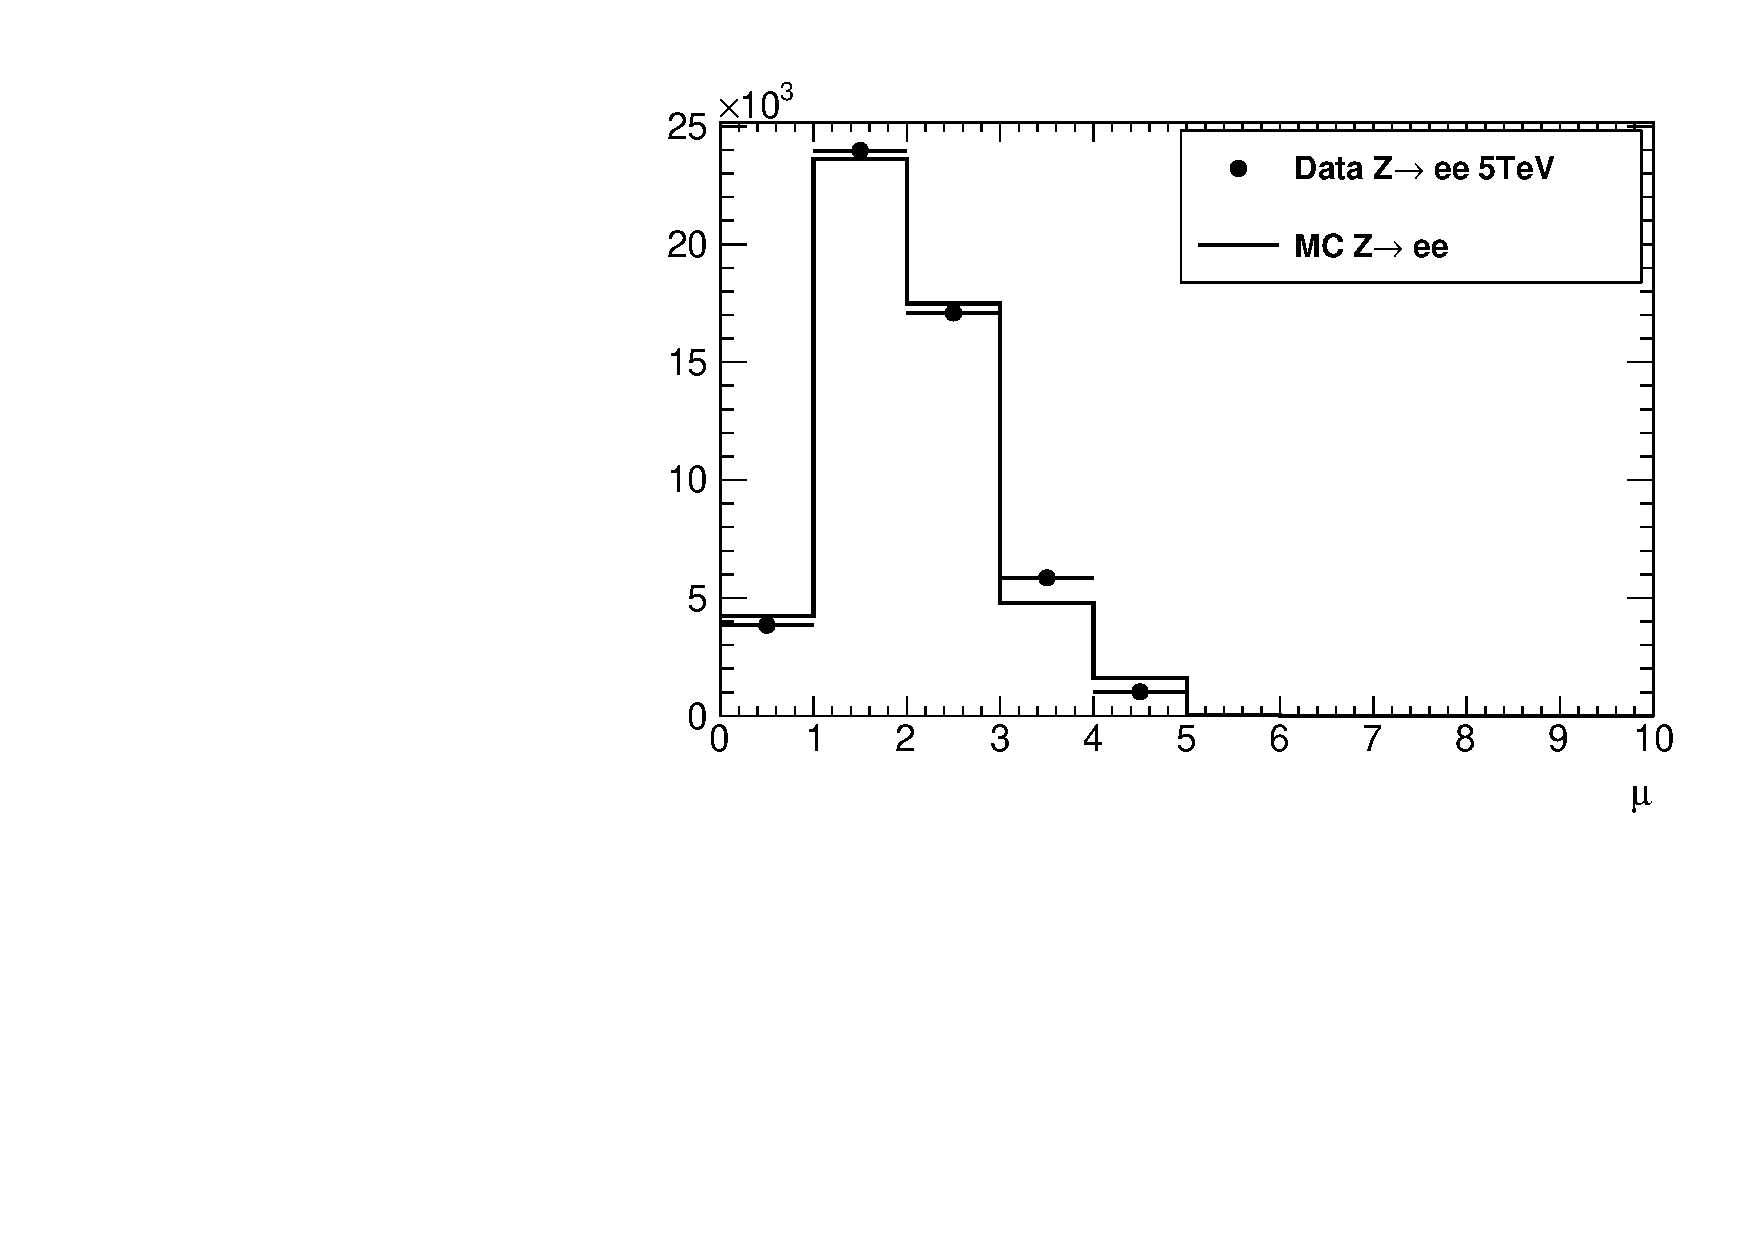
\includegraphics[width=.33\textwidth]{zee_5tev_mu.pdf}%
		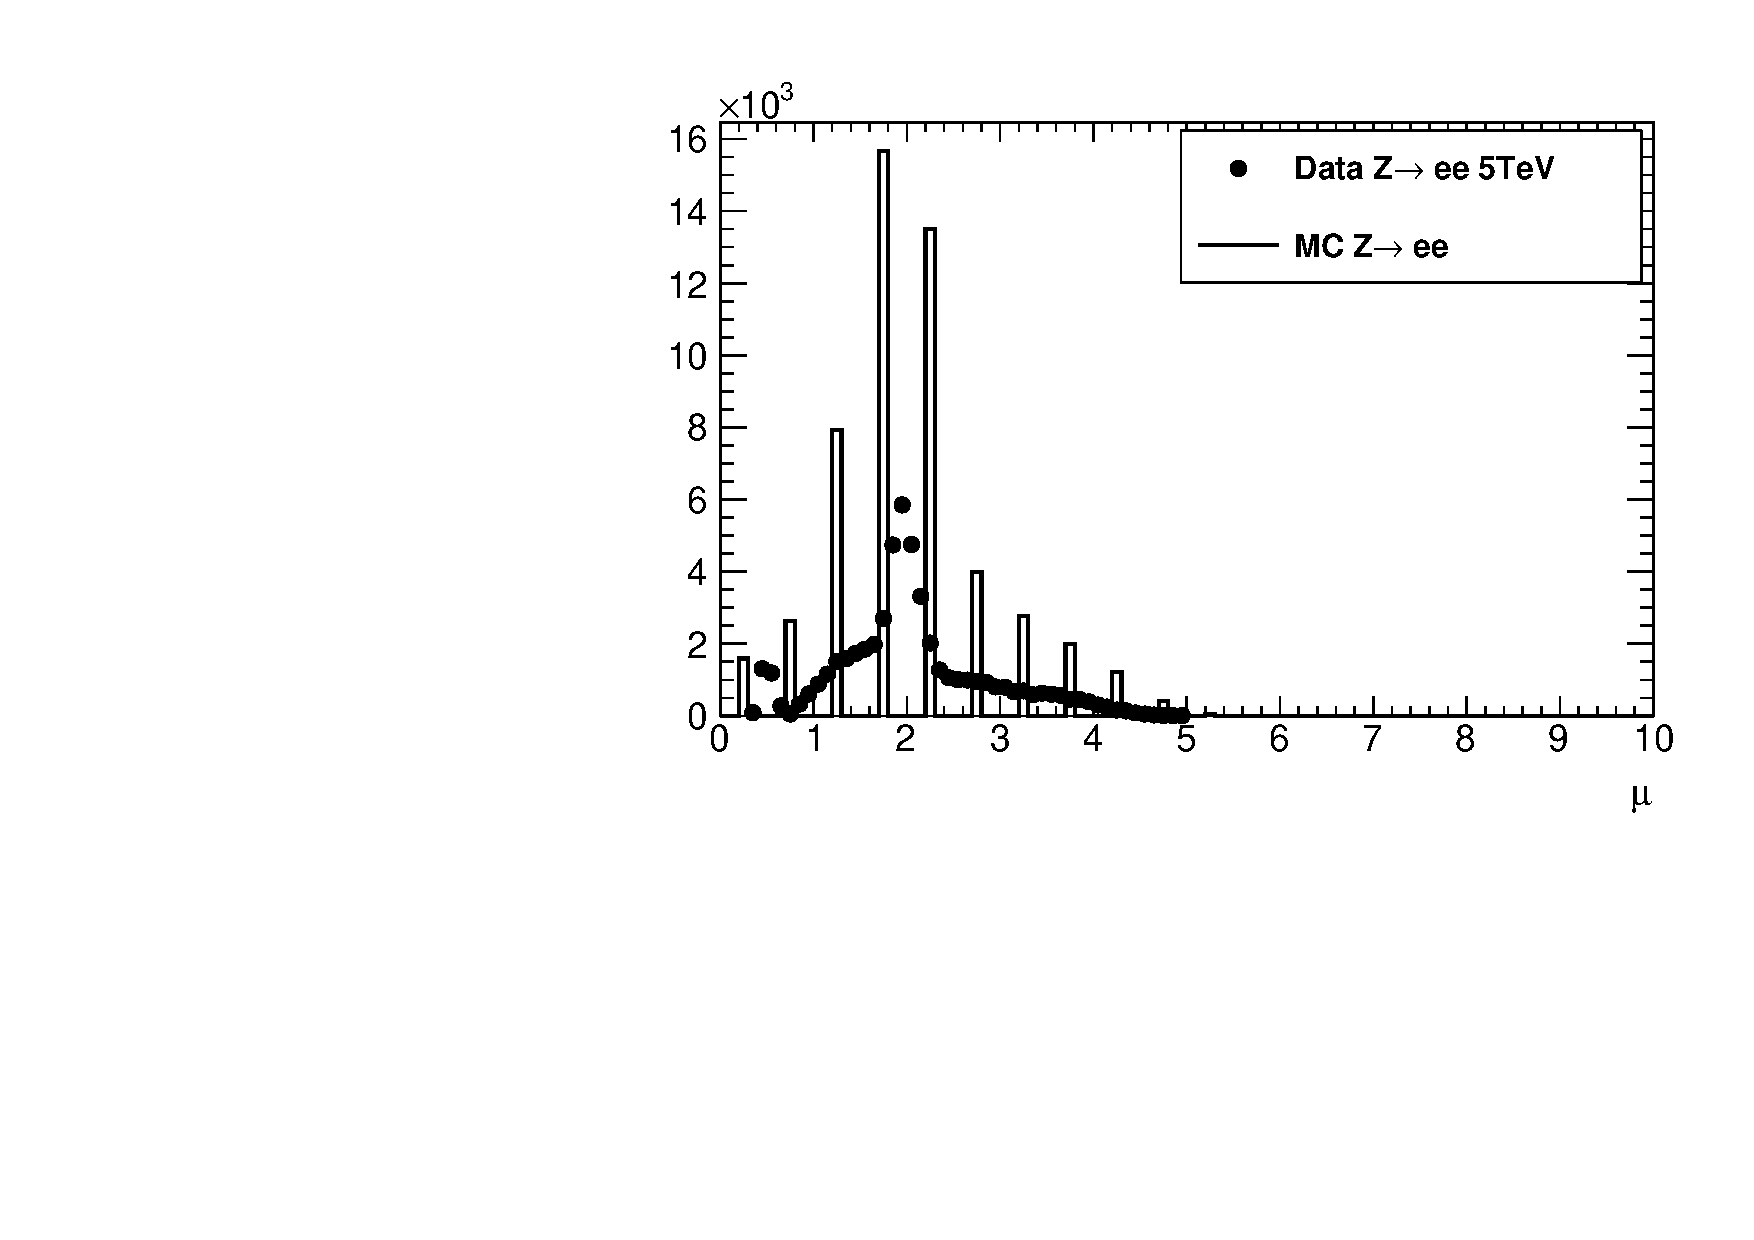
\includegraphics[width=.33\textwidth]{zee_5tev_mufine.pdf}%
		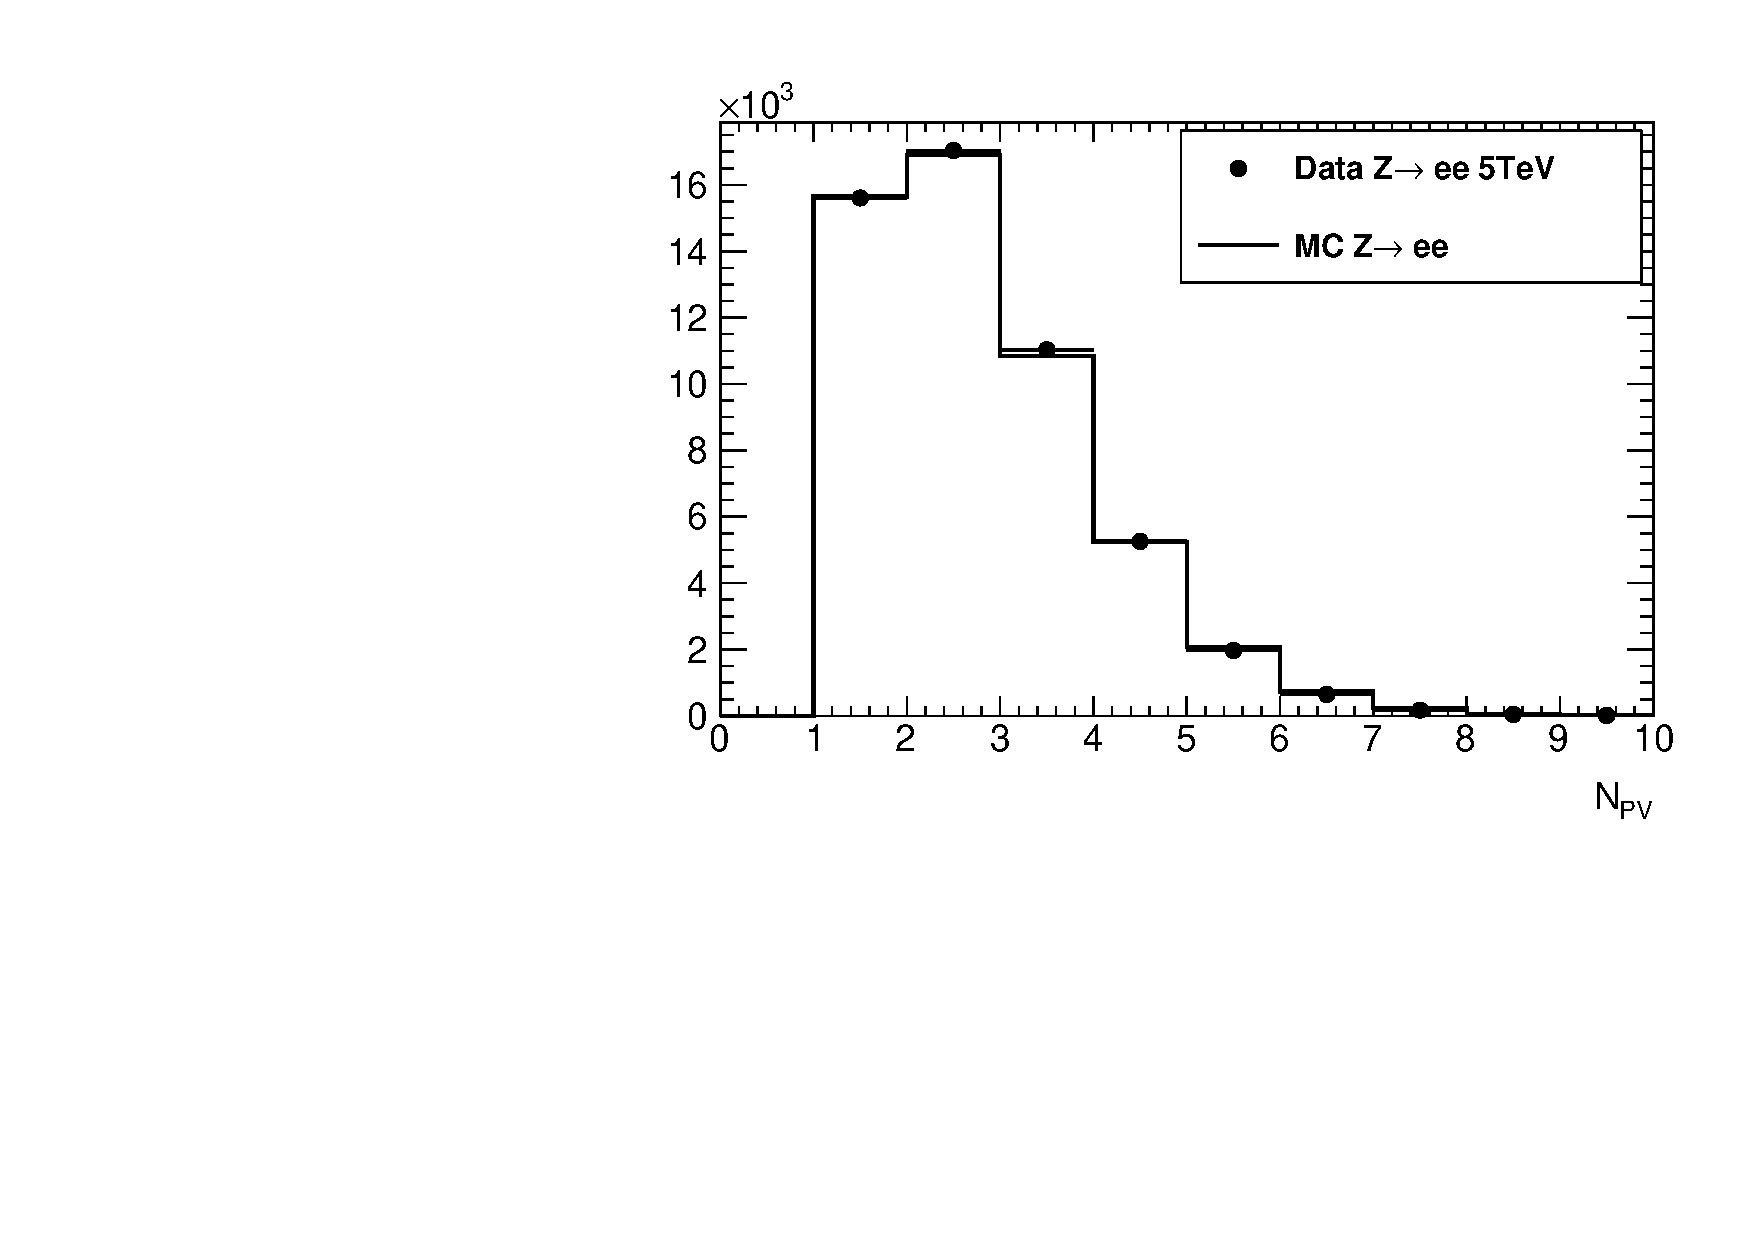
\includegraphics[width=.33\textwidth]{zee_5tev_npv}
		\caption{Distributions for the 5 TeV low-$\mu$ dataset in a $\Zgmm$
			(top row) and a \Zgee (bottom row) selection. The data (points) is
			compared to \Zgmm or \Zgee signal MC, respectively. The left and
			middle plots show the actual $\mu$ in a coarsely-binned and a
			finely-binned version. The right plot shows the number of
			reconstructed primary vertices $N_{PV}$~\cite{int_note_samples}.}
		\label{fig:mu5}
	\end{figure}
	
	\begin{figure}[tph]
		\centering
		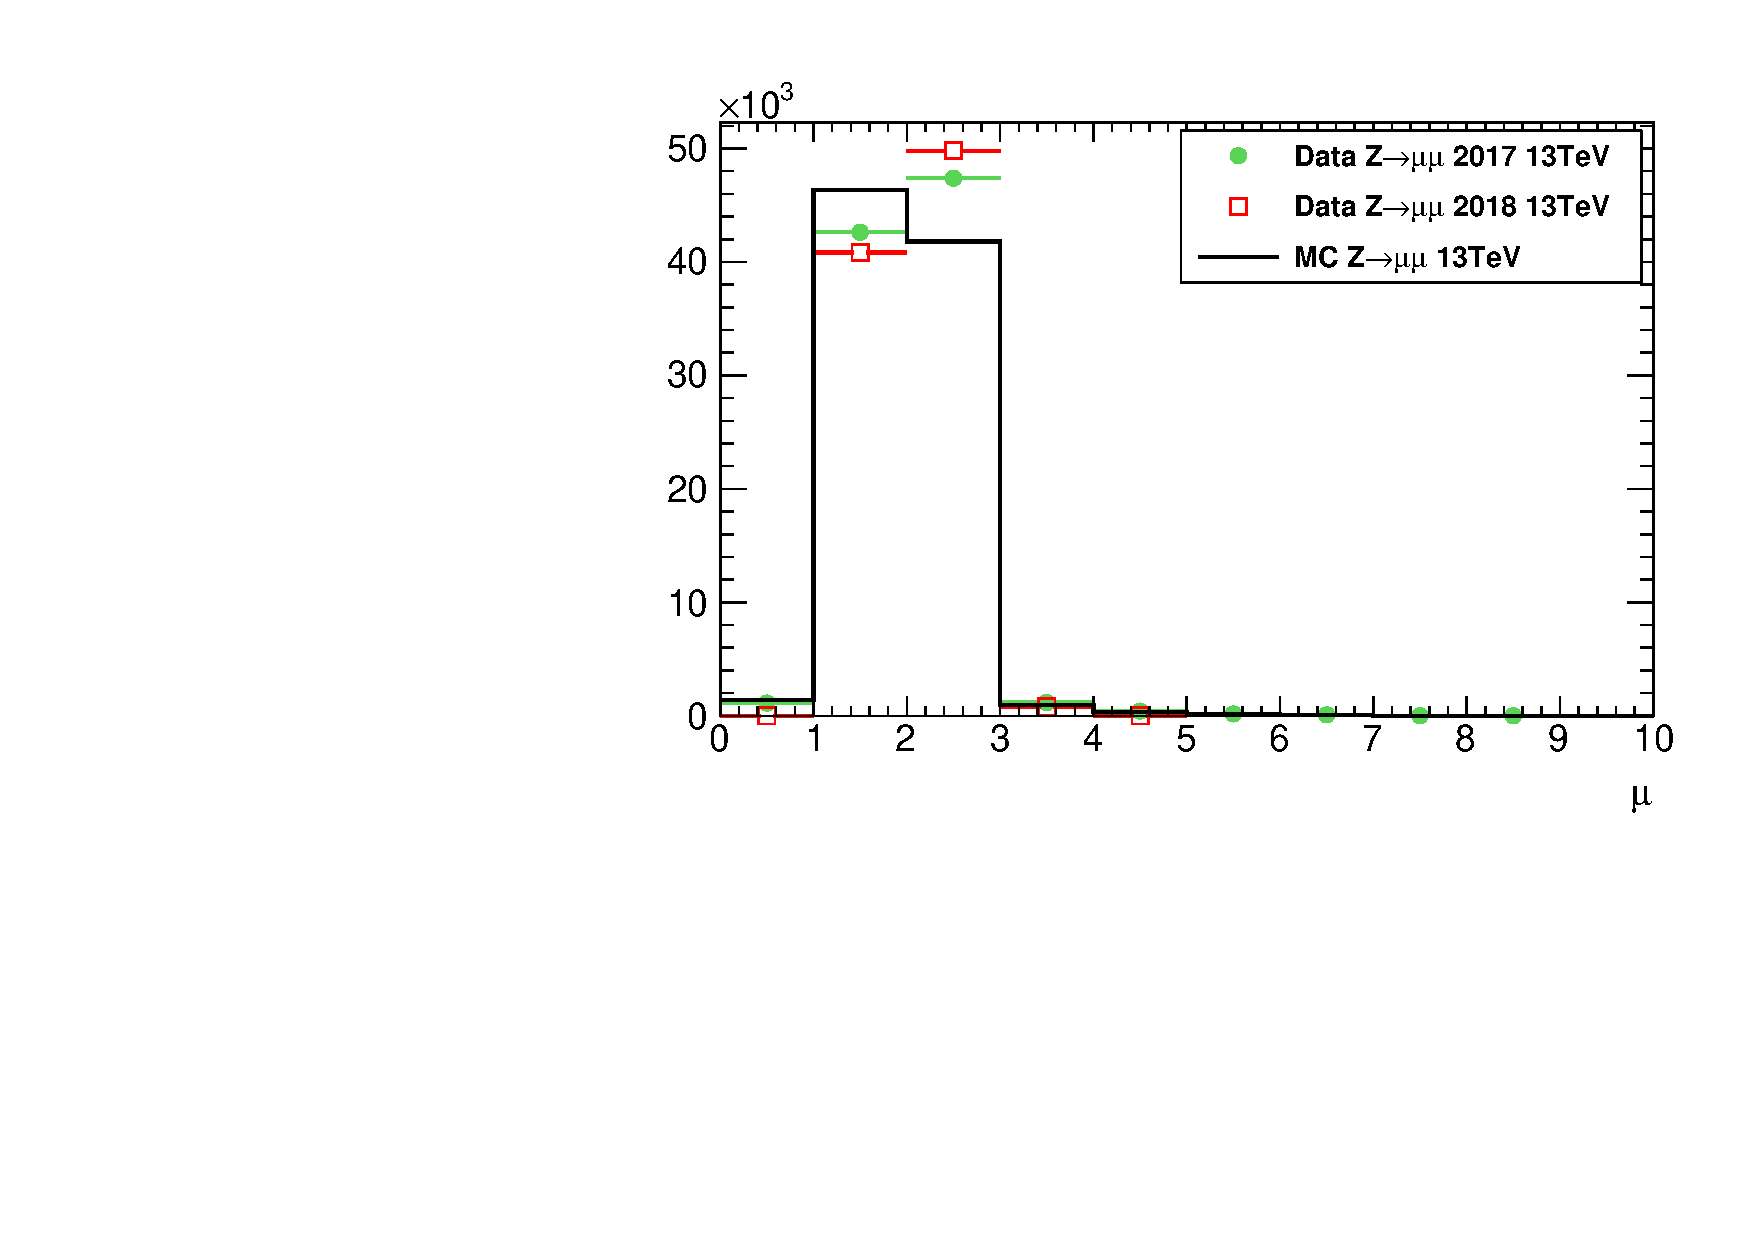
\includegraphics[width=.33\textwidth]{zmumu_13tev_mu}%
		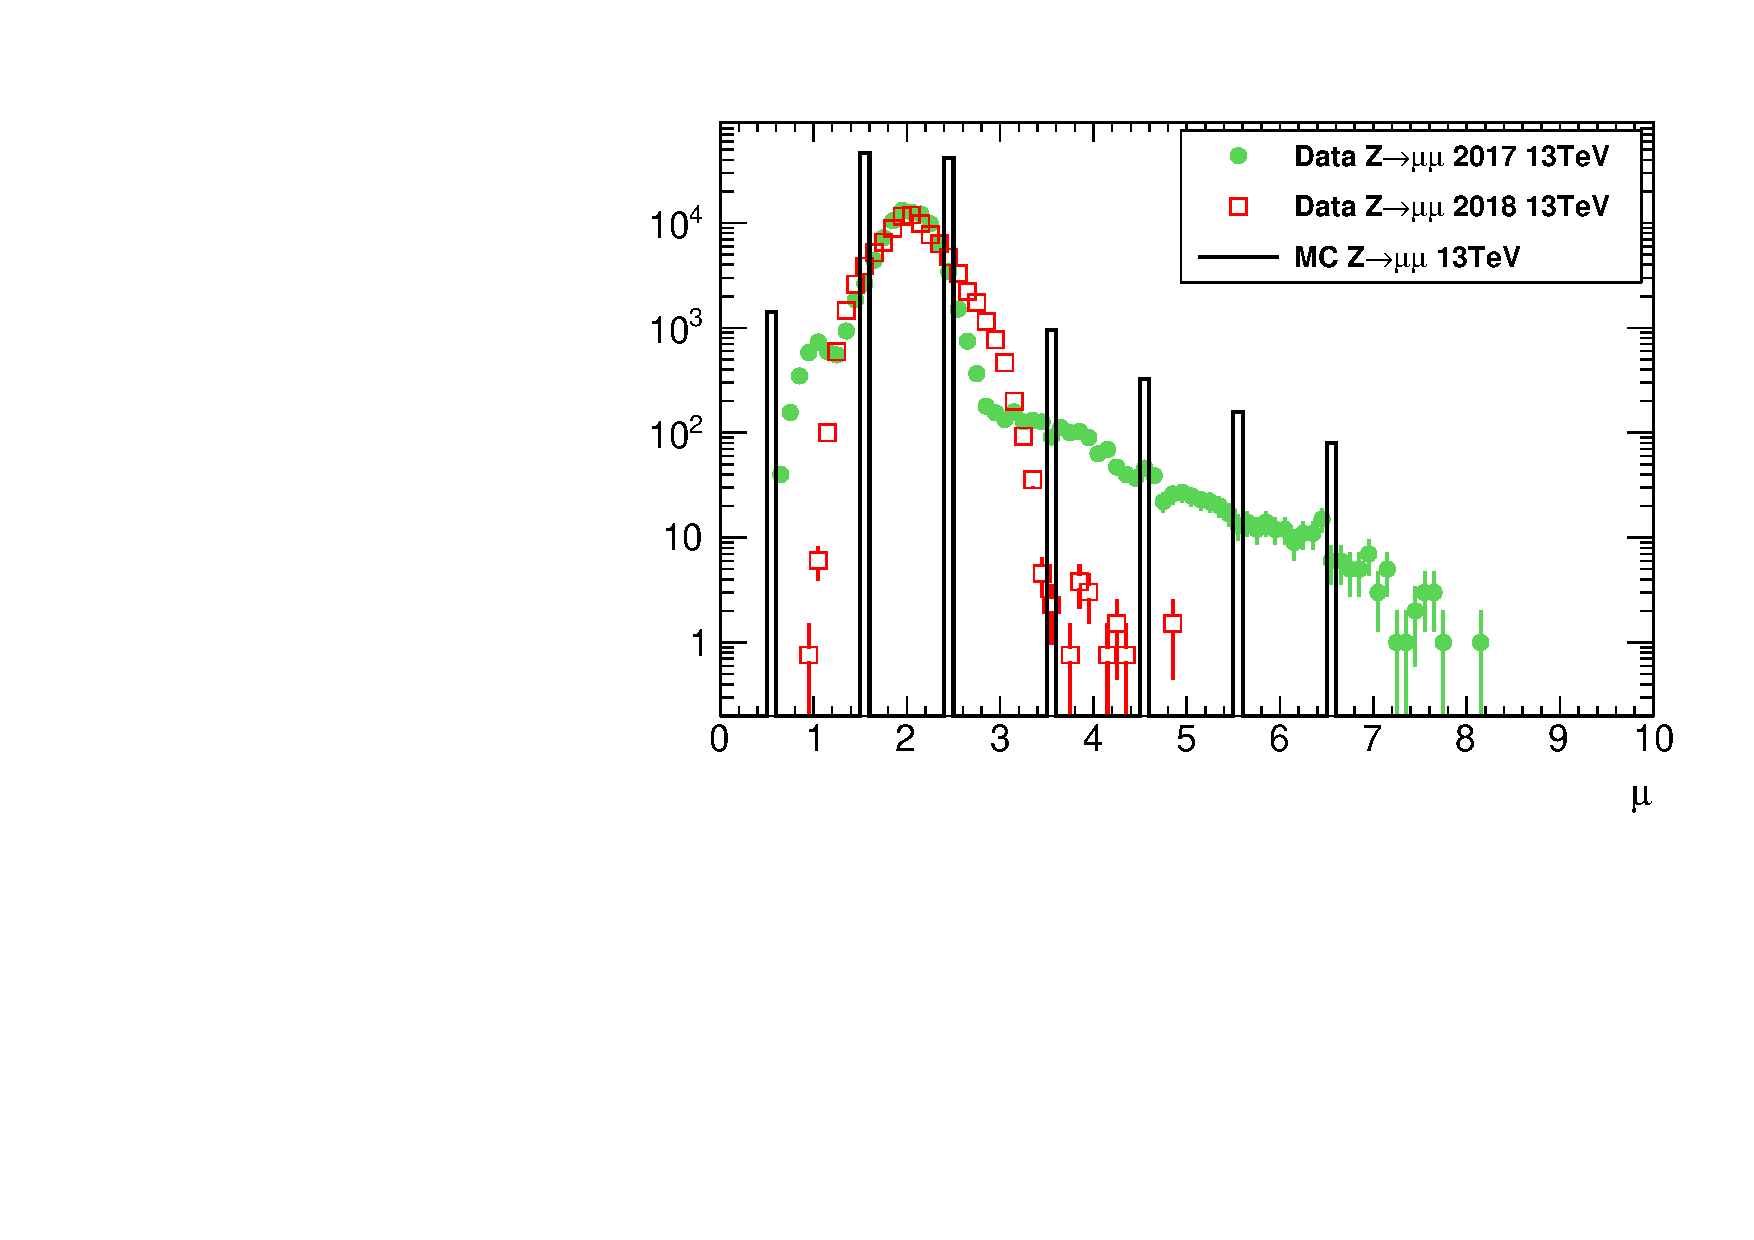
\includegraphics[width=.33\textwidth]{zmumu_13tev_mufine_log}%
		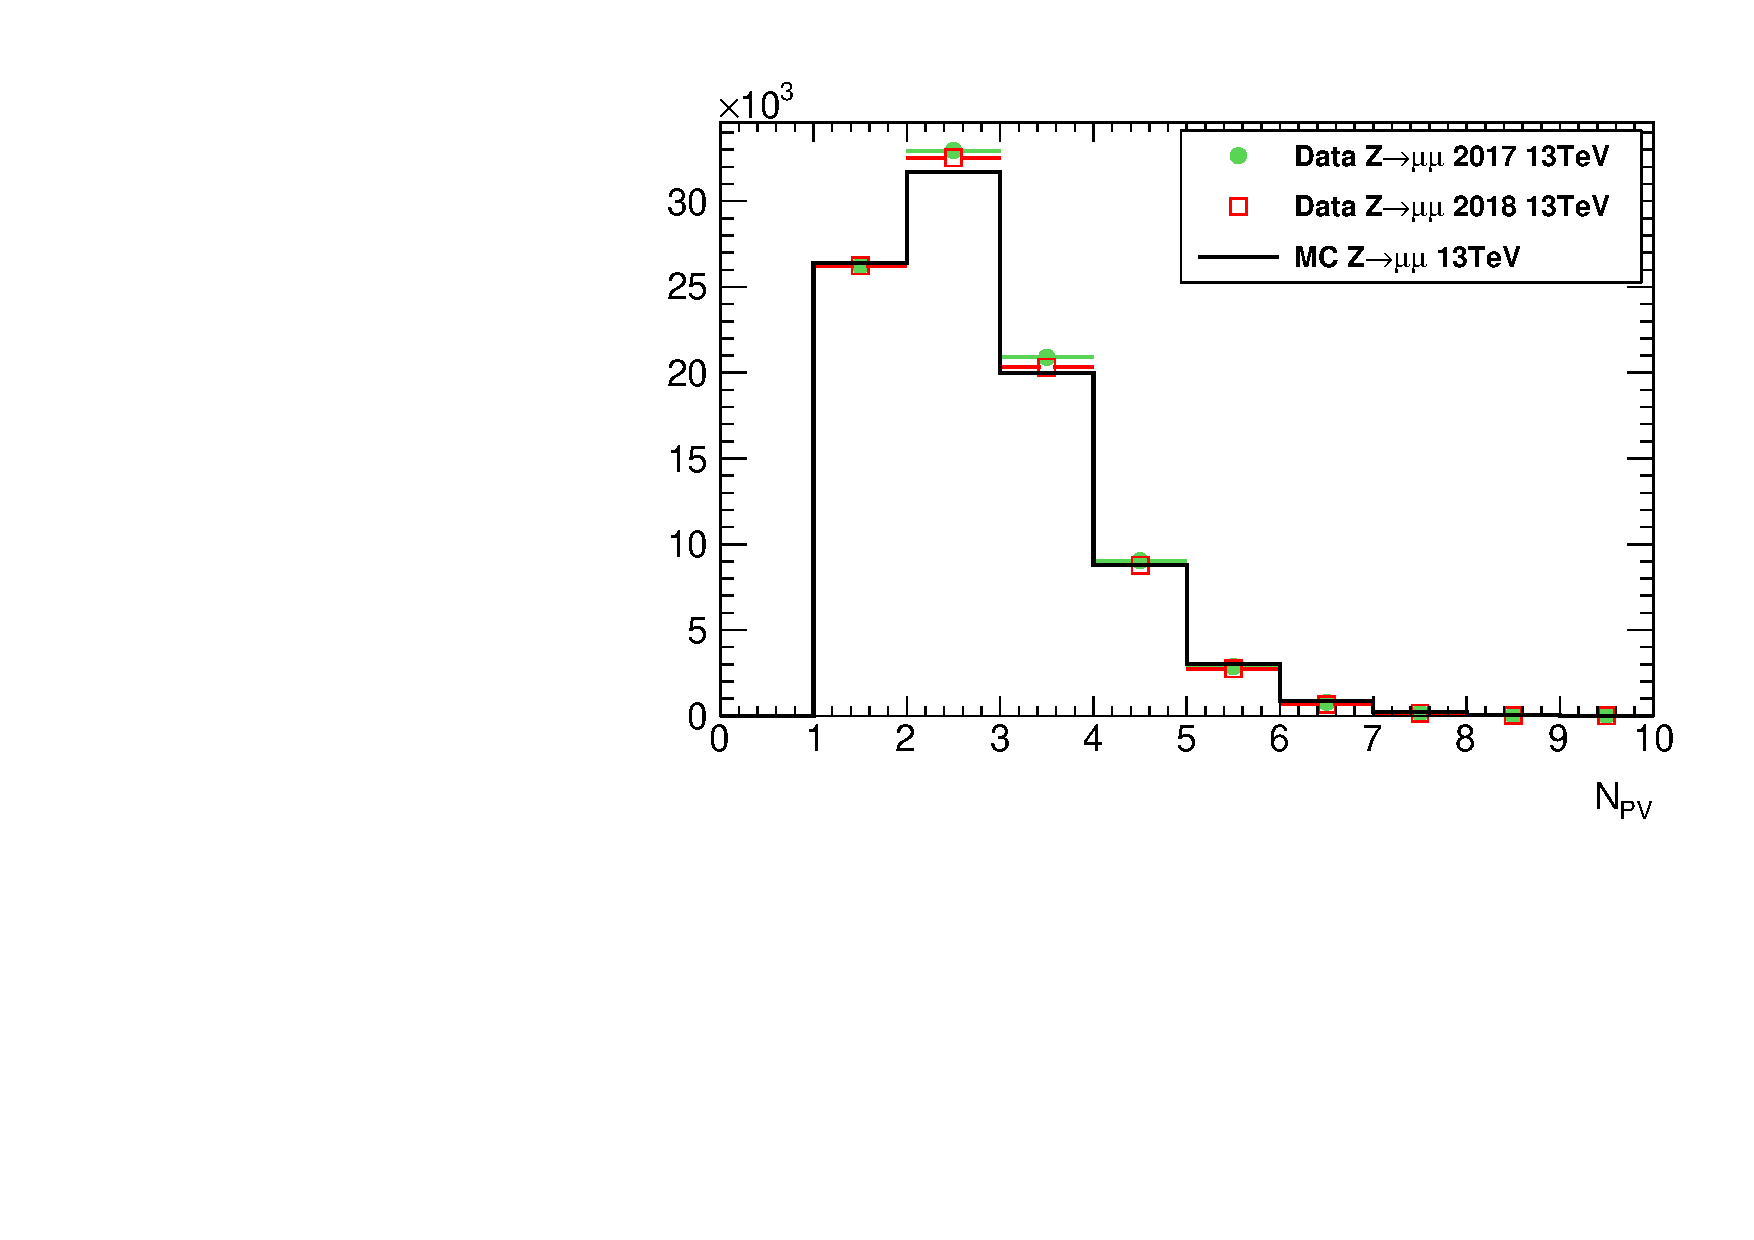
\includegraphics[width=.33\textwidth]{zmumu_13tev_npv}
		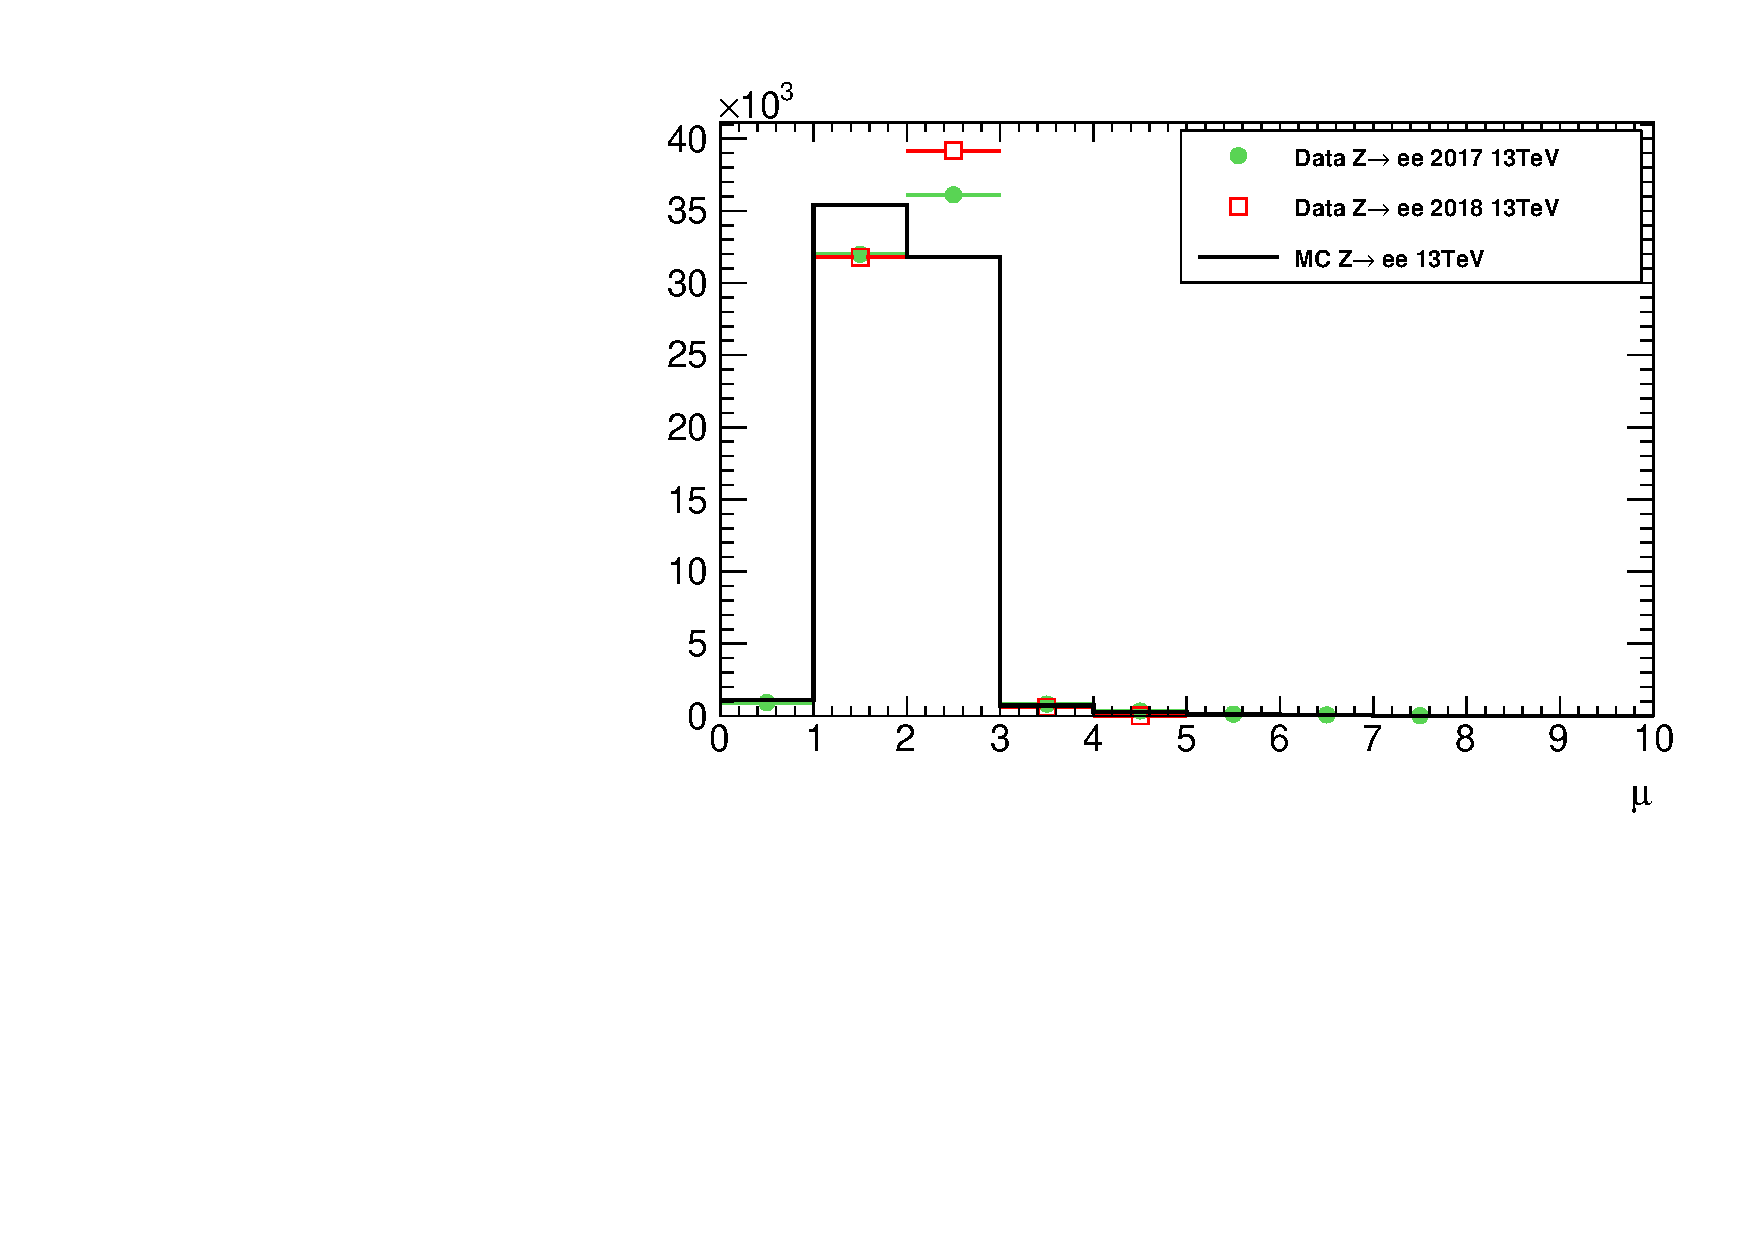
\includegraphics[width=.33\textwidth]{zee_13tev_mu}%
		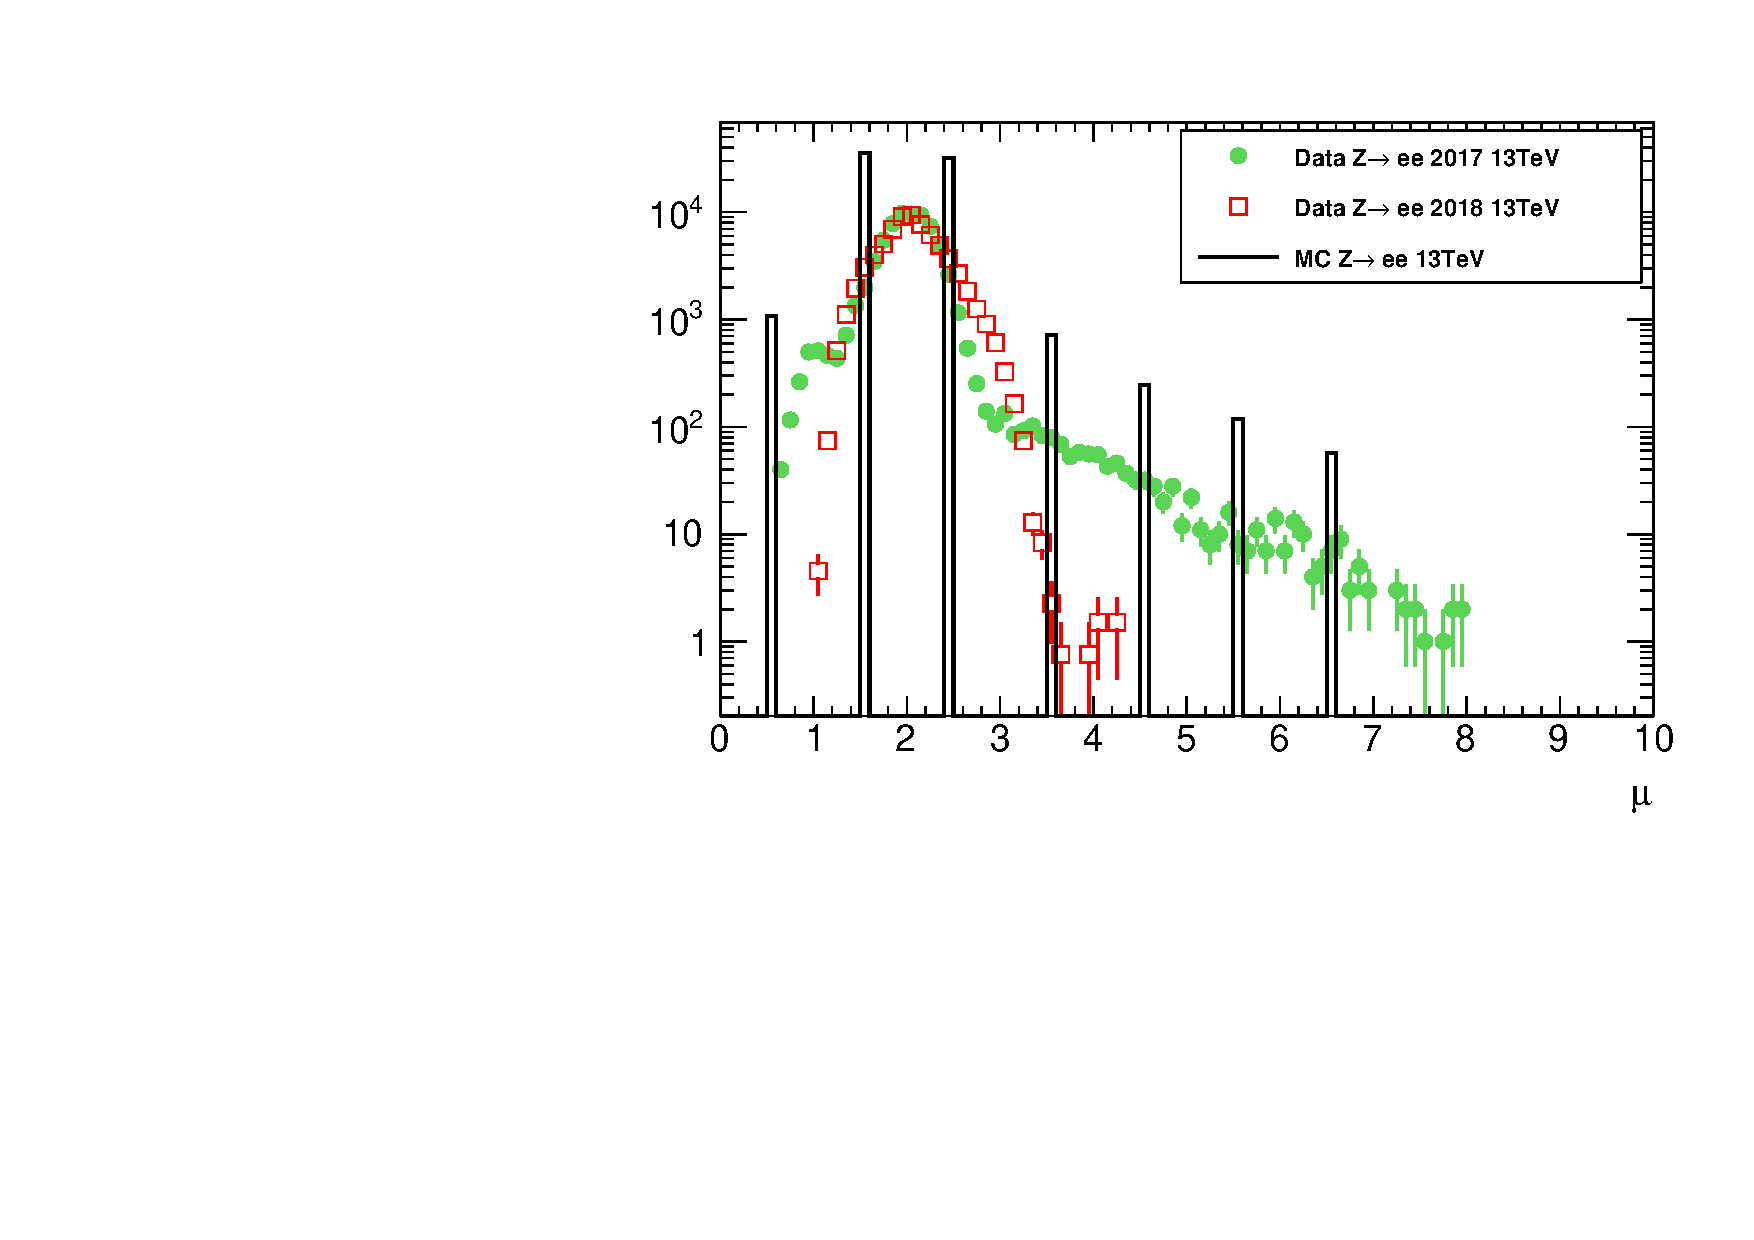
\includegraphics[width=.33\textwidth]{zee_13tev_mufine_log}%
		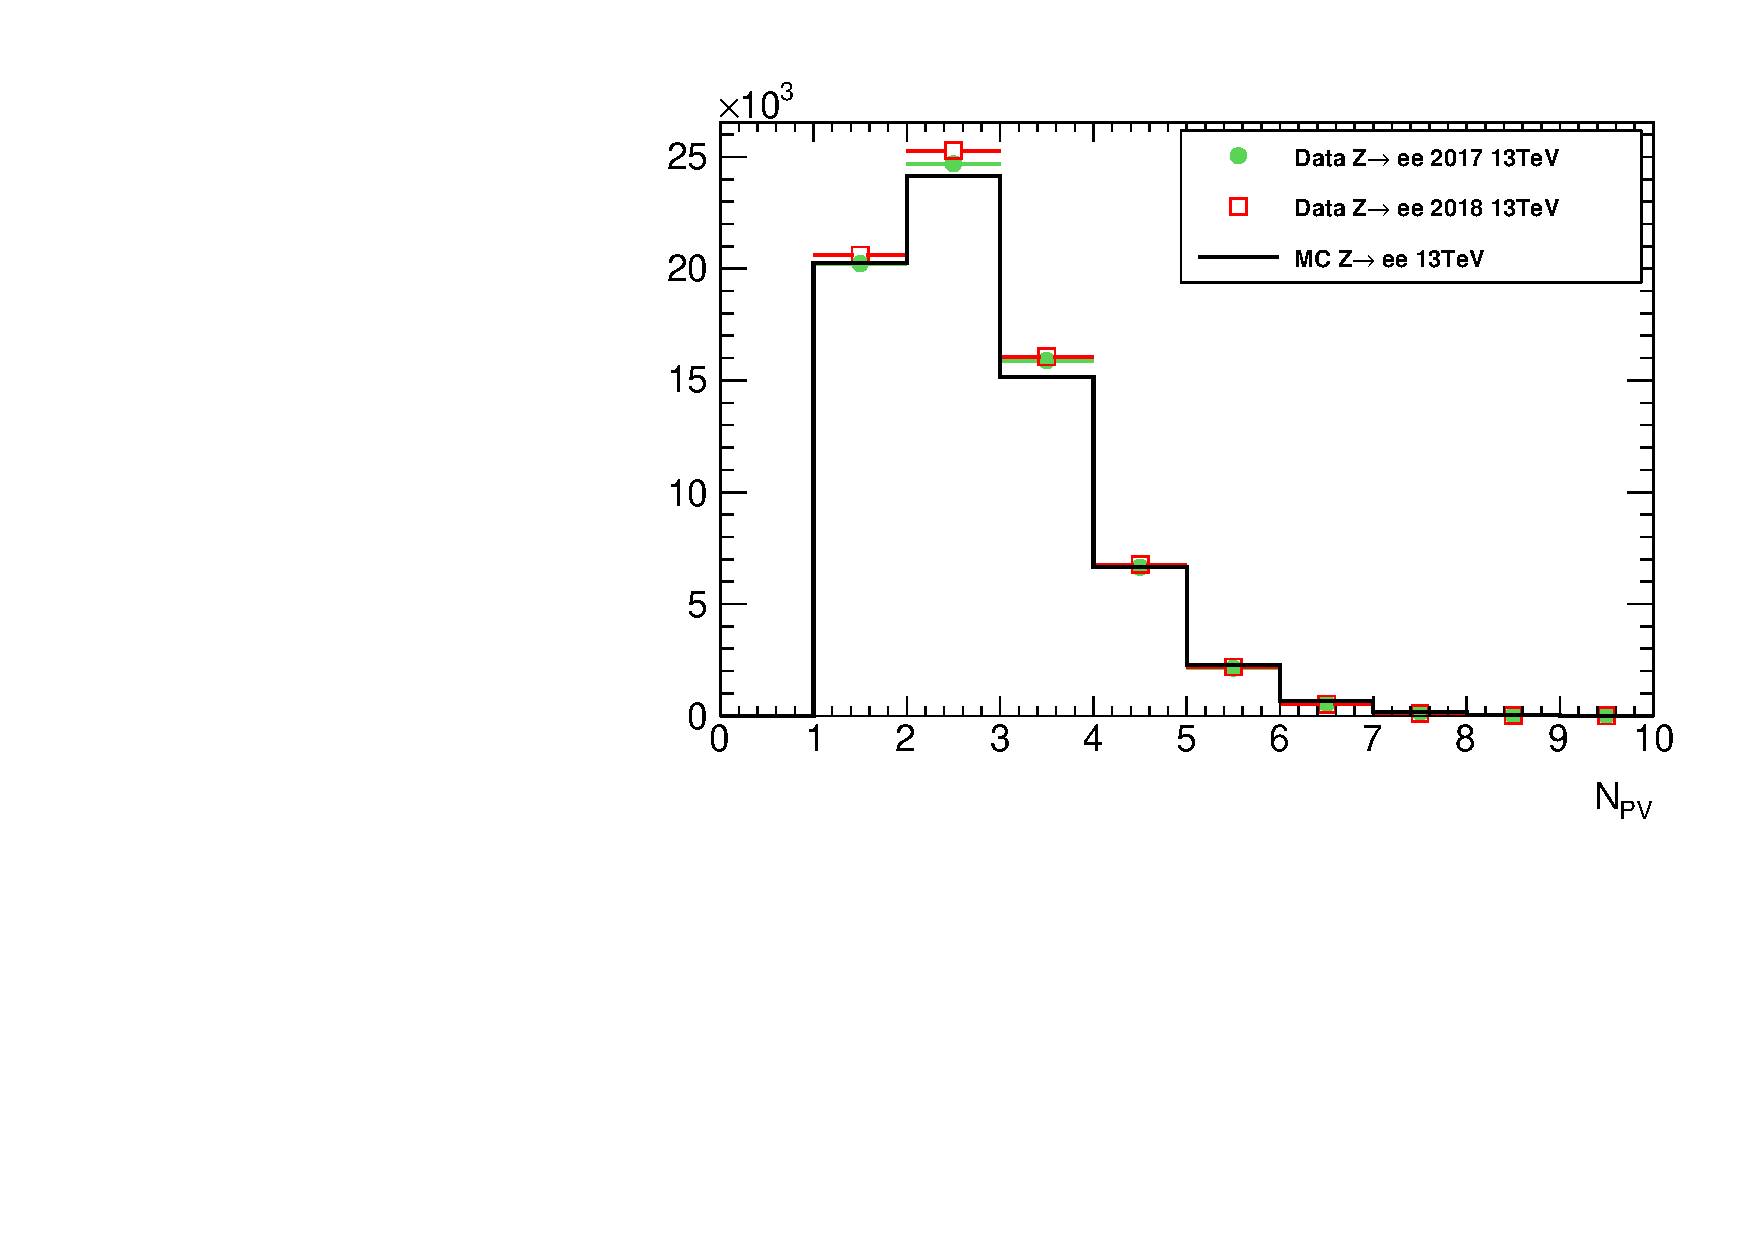
\includegraphics[width=.33\textwidth]{zee_13tev_npv}
		\caption{Distributions for the 13 TeV low-$\mu$ datasets taken in
			2017 and 2018 in a \Zgmm (top row) and a \Zgee (bottom row)
			selection. The data (points) is compared to \Zgmm or \Zgee signal
			MC, respectively. All distributions are (roughly) normalised to
			the same number of selected events in the 2017 dataset. The left
			and middle plots show the actual $\mu$ in a coarsely-binned and a
			finely-binned version. The right plot shows the number of
			reconstructed primary vertices $N_{PV}$~\cite{int_note_samples}.}
		\label{fig:mu13}
	\end{figure}
	
    \subsection{MC samples and cross-sections}
    Signal and background processes (except for the multijet background) are modelled using fully simulated and reconstructed \gls{mc} samples, specifically tuned for the special run conditions, namely the low pileup, lower topo-cluster noise thresholds and adapted trigger menu. No pileup reweighting is performed.
    
    The information on the simulated samples and their properties is given in Tables \ref{tab:samples13}, \ref{tab:samples13_sherpaz}, \ref{tab:samples13_sherpaw},  \ref{tab:samples5} \cite{Kretzschmar:2657141}. The predicted event counts are normalized to the data luminosity using the cross-sections quoted in the table.
    
    The primary signal event samples for W and Z production are obtained using \Powheg~\cite{Nason:2004rx,Frixione:2007vw,Alioli:2008gx,Alioli:2010xd} event generator with CT10 PDF, linked with \Pythia~\cite{pythia} with AZNLO tune~\cite{STDM-2012-23}. \Powheg+\Pythia samples are interfaced to \Photos~\cite{Golonka:2005pn}  for final state \gls{qed} effects simulation.
    
    A set of alternative samples at $\sqrt{s} = 13\tev$ was prepared with \Sherpa 2.2.2~\cite{Hoche:2010kg} using the NNPDF3.0 PDFs and merging
    $V+0,1,2$ at NLO accuracy with $V+3,4$ at LO accuracy with the MEPS@NLO scheme. A similar set for $\sqrt{s} = 5\tev$ was prepared with \Sherpa 2.2.5 with a setup similar to 13 TeV samples.
    
    Pileup is modelled by overlaying simulated soft events over the original hard-scattering event. These soft events were modelled using \Pythia\ with NNPDF2.3LO set of PDFs~\cite{Ball:2012cx} and the A3 tune~\cite{ATL-PHYS-PUB-2016-017}.
    
    The $W$ and $Z$ processes samples are normalized to NNLO
    calculations for the cross-sections performed using DYTURBO, an optimised version
    of DYRES~\cite{Catani:2007vq,Catani:2009sm} using the MMHT2014nnlo PDF
    set~\cite{Harland-Lang:2014zoa}. Corresponding numerical values were taken from
    the corresponding ATLAS publications of the 2015 data at 13
    TeV~\cite{STDM-2015-03} and 5.02 TeV~\cite{HION-2018-02} and are presented in Table~\ref{tab:samples13} for 13 TeV and Table~\ref{tab:samples5} for 5 TeV. The
    uncertainties on those cross-sections arise from the choice of PDF set, from factorization
    and renormalisation scale dependence, and the strong
    coupling constant $\alpha_s$ uncertainty resulting in the total 
    uncertainty estimate of about $5\%$.
    
    Backgrounds from top-quark pair-production $t\bar{t}$ and 
    single-top production ($Wt$, t-channel, s-channel) were generated with
    \Powheg+\Pythia.
    The 5 TeV $t\bar{t}$ cross section is taken as the \textsc{Top++}~\cite{Czakon:2011xx} prediction reported in CMS publication~\cite{CMS-TOP-16-023}.
    Di-boson combinations $VV, V=W,Z$ are generated with \Sherpa\ in all decay channels with a requirement of having at least one real lepton in the final state.
    
    \begin{table}[htbp]
    	\begin{center}
    		\begin{tabular}{l|l|l|l|l|l}
    			\hline
    			\hline
    			Process & Data set & Generator& $\sigma{\cdot}
    			\text{BR}{\cdot}\epsilon_\mathrm{filter}$ [nb] (th. unc.)
    			& $N^\mathrm{skim}_\mathrm{evt}\,[10^6]$
    			& $N^\mathrm{unskim}_\mathrm{evt}\,[10^6]$\\
    			\hline\hline
    			$ W^{+} \to e^{+}\nu $ & 361100 & \Powheg+\Pythia & 11.61 (5\%)  & 40 & 40 \\\hline
    			$ W^{+} \to \mu^{+}\nu $ & 361101 & \Powheg+\Pythia & 11.61 (5\%)  & 40 & 40 \\\hline
    			$ W^{+} \to \tau^{+}\nu $ & 361102 & \Powheg+\Pythia & 11.61 (5\%)  & 0.28 & 5.0 \\\hline
    			$ W^{-} \to e^{-}\bar{\nu} $ & 361103 & \Powheg+\Pythia & 8.630 (5\%)  & 30 & 30 \\\hline
    			$ W^{-} \to \mu^{-}\bar{\nu} $ & 361104 & \Powheg+\Pythia & 8.630 (5\%)  & 29 & 29 \\\hline
    			$ W^{-} \to \tau^{-}\bar{\nu} $ & 361105 & \Powheg+\Pythia & 8.630 (5\%)  & 0.24 & 4.0 \\\hline\hline
    			$ Z \to ee $ & 361106 & \Powheg+\Pythia & 1.910 $\times$ 1.03 (5\%)  & 10 & 10 \\\hline
    			$ Z \to \mu\mu $ & 361107 & \Powheg+\Pythia & 1.910 $\times$ 1.025 (5\%)  & 10 & 10 \\\hline
    			$ Z \to \tau\tau $ & 361108 & \Powheg+\Pythia & 1.910 $\times$ 1.025 (5\%)  & 0.12 & 1.0 \\\hline\hline
    			$ ZZ (q\bar{q}\ell\ell) $ & 363356 & \Sherpa\ 2.2.1 & 0.01556 $\times$ 0.141 (10\%)  & 0.0064 & 0.010 \\\hline
    			$ WZ (q\bar{q}\ell\ell) $ & 363358 & \Sherpa\ 2.2.1 & 0.003433 (10\%)  & 0.0063 & 0.010 \\\hline
    			$ WW (q\bar{q}\ell\nu) $ & 363359 & \Sherpa\ 2.2.1 & 0.02472 (10\%)  & 0.0093 & 0.020 \\\hline
    			$ WW (\ell\nu q\bar{q}) $ & 363360 & \Sherpa\ 2.2.1 & 0.02472 (10\%)  & 0.0093 & 0.020 \\\hline
    			$ WZ (\ell\nu q\bar{q}) $ & 363489 & \Sherpa\ 2.2.1 & 0.01142 (10\%)  & 0.0047 & 0.010 \\\hline
    			$ ZZ (4\ell) $ & 364250 & \Sherpa\ 2.2.2 & 0.001252 (10\%)  & 0.0057 & 0.010 \\\hline
    			$ WZ (3\ell\nu) $ & 364253 & \Sherpa\ 2.2.2 & 0.004583 (10\%)  & 0.0062 & 0.010 \\\hline
    			$ WW (2\ell 2\nu) $ & 364254 & \Sherpa\ 2.2.2 & 0.01250 (10\%)  & 0.0073 & 0.010 \\\hline
    			$ WZ (\ell 3\nu) $ & 364255 & \Sherpa\ 2.2.2 & 0.003235 (10\%)  & 0.0050 & 0.010 \\\hline\hline
    			$ Wt $ & 410013 & \Powheg+\Pythia & 0.03582 (10\%)  & 0.0037 & 0.010 \\\hline
    			$ W\bar{t} $ & 410014 & \Powheg+\Pythia & 0.03399 (10\%)  & 0.0037 & 0.010 \\\hline
    			$ t\bar{t} $ (nominal) & 410470 & \Powheg+\Pythia & 0.8318 $\times$ 0.544 (7\%)  & 1.2 & 2.0 \\\hline
    			$ t (\mathrm{t-chan.} t) $ & 410642 & \Powheg+\Pythia & 0.03699 (10\%)  & 0.016 & 0.030 \\\hline
    			$ t (\mathrm{t-chan.} \bar{t}) $ & 410643 & \Powheg+\Pythia & 0.02217 (10\%)  & 0.011 & 0.020 \\\hline
    			$ t (\mathrm{s-chan.} t) $ & 410644 & \Powheg+\Pythia & 0.002027 (10\%)  & 0.0050 & 0.010 \\\hline
    			$ t (\mathrm{s-chan.} \bar{t}) $ & 410645 & \Powheg+\Pythia & 0.001268 (10\%)  & 0.0052 & 0.010 \\\hline\hline
    			$ t\bar{t} $ (syst.) & 410480 & \Powheg+\Pythia & 0.8318 $\times$ 0.438 (7\%)  & 0.85 & 1.5 \\\hline
    			$ t\bar{t} $ (syst.) & 410482 & \Powheg+\Pythia & 0.8318 $\times$ 0.105 (7\%)  & 0.40 & 0.50 \\\hline
    			$ t\bar{t} $ (syst.) & 410557 & \Powheg+\Pythia & 0.8318 $\times$ 0.438 (7\%)  & 0.85 & 1.5 \\\hline
    			$ t\bar{t} $ (syst.) & 410558 & \Powheg+\Pythia & 0.8318 $\times$ 0.105 (7\%)  & 0.40 & 0.50 \\\hline
    			\hline
    		\end{tabular}
    		\caption{Monte Carlo samples at $\sqrt{s} = 13\tev$. Given is a
    			short description of the process, the ATLAS MC data set number
    			(DSID), the names and version numbers of the MC generator(s),
    			the used value of the higher order cross section times
    			any branching and filter efficiencies ($\sigma{\cdot}
    			\text{BR}{\cdot}\epsilon_\mathrm{filter}$) with the
    			theoretical uncertainty in percent (``th. unc.''),
    			and finally the number of events analysed
    			after skimming at derivation production
    			($N^\mathrm{skim}_\mathrm{evt}$) as well as the number of events
    			originally processed and simulated
    			($N^\mathrm{unskim}_\mathrm{evt}$). In the case of
    			$Z\to\ell\ell$ samples, the given $\epsilon_\mathrm{filter} > 1$
    			is related to the fact, that the cross sections were calculated
    			for $66 <m_{\ell\ell} <116\gev$, but the generated mass range is
    			larger. The last section of $t\bar{t}$ samples refers to
    			variation samples for systematics studies. The MC equivalent
    			luminosity
    			$N^\mathrm{unskim}_\mathrm{evt}/(\sigma{\cdot}\text{BR}{\cdot}\epsilon_\mathrm{filter})$
    			is generally above $3\ifb$ for signal and significant
    			backgrounds, the exception are Powheg $W\to\tau\nu$ and
    			$Z\to\tau\tau$ samples, that have about $0.45\ifb$ only~\cite{int_note_samples}.}
    		\label{tab:samples13}
    	\end{center}
    \end{table}
    
    \begin{table}[htbp]
    	\begin{center}
    		\begin{tabular}{l|l|l|l|l|l}
    			\hline
    			\hline
    			Process & Data set & Generator& $\sigma{\cdot}
    			\text{BR}{\cdot}\epsilon_\mathrm{filter}$ [nb] (th. unc.)
    			& $N^\mathrm{skim}_\mathrm{evt}\,[10^6]$
    			& $N^\mathrm{unskim}_\mathrm{evt}\,[10^6]$\\
    			\hline\hline
    			$ Z \to \mu\mu $ & 364100 & \Sherpa\ 2.2.1 & 1.932 $\times$ 0.822 (5\%)  & 8.0 & 8.0 \\\hline
    			$ Z \to \mu\mu $ & 364101 & \Sherpa\ 2.2.1 & 1.933 $\times$ 0.114 (5\%)  & 1.5 & 1.5 \\\hline
    			$ Z \to \mu\mu $ & 364102 & \Sherpa\ 2.2.1 & 1.932 $\times$ 0.0660 (5\%)  & 1.1 & 1.1 \\\hline
    			$ Z \to \mu\mu $ & 364103 & \Sherpa\ 2.2.1 & 0.1063 $\times$ 0.690 (5\%)  & 1.5 & 1.5 \\\hline
    			$ Z \to \mu\mu $ & 364104 & \Sherpa\ 2.2.1 & 0.1062 $\times$ 0.200 (5\%)  & 0.40 & 0.40 \\\hline
    			$ Z \to \mu\mu $ & 364105 & \Sherpa\ 2.2.1 & 0.1063 $\times$ 0.114 (5\%)  & 0.25 & 0.25 \\\hline
    			$ Z \to \mu\mu $ & 364106 & \Sherpa\ 2.2.1 & 0.03889 $\times$ 0.593 (5\%)  & 0.20 & 0.20 \\\hline
    			$ Z \to \mu\mu $ & 364107 & \Sherpa\ 2.2.1 & 0.03885 $\times$ 0.235 (5\%)  & 0.060 & 0.060 \\\hline
    			$ Z \to \mu\mu $ & 364108 & \Sherpa\ 2.2.1 & 0.03889 $\times$ 0.156 (5\%)  & 0.035 & 0.035 \\\hline
    			$ Z \to \mu\mu $ & 364109 & \Sherpa\ 2.2.1 & 0.008310 $\times$ 0.561 (5\%)  & 0.020 & 0.020 \\\hline
    			$ Z \to \mu\mu $ & 364110 & \Sherpa\ 2.2.1 & 0.008310 $\times$ 0.266 (5\%)  & 0.010 & 0.010 \\\hline
    			$ Z \to \mu\mu $ & 364111 & \Sherpa\ 2.2.1 & 0.008320 $\times$ 0.177 (5\%)  & 0.0050 & 0.0050 \\\hline
    			$ Z \to \mu\mu $ & 364112 & \Sherpa\ 2.2.1 & 0.001740 (5\%)  & 0.0050 & 0.0050 \\\hline
    			$ Z \to \mu\mu $ & 364113 & \Sherpa\ 2.2.1 & 0.0001400 (5\%)  & 0.0050 & 0.0050 \\\hline
    			$ Z \to ee $ & 364114 & \Sherpa\ 2.2.1 & 1.933 $\times$ 0.821 (5\%)  & 8.0 & 8.0 \\\hline
    			$ Z \to ee $ & 364115 & \Sherpa\ 2.2.1 & 1.932 $\times$ 0.114 (5\%)  & 1.5 & 1.5 \\\hline
    			$ Z \to ee $ & 364116 & \Sherpa\ 2.2.1 & 1.932 $\times$ 0.0658 (5\%)  & 1.1 & 1.1 \\\hline
    			$ Z \to ee $ & 364117 & \Sherpa\ 2.2.1 & 0.1080 $\times$ 0.694 (5\%)  & 1.5 & 1.5 \\\hline
    			$ Z \to ee $ & 364118 & \Sherpa\ 2.2.1 & 0.1077 $\times$ 0.191 (5\%)  & 0.40 & 0.40 \\\hline
    			$ Z \to ee $ & 364119 & \Sherpa\ 2.2.1 & 0.1078 $\times$ 0.119 (5\%)  & 0.25 & 0.25 \\\hline
    			$ Z \to ee $ & 364120 & \Sherpa\ 2.2.1 & 0.03964 $\times$ 0.616 (5\%)  & 0.20 & 0.20 \\\hline
    			$ Z \to ee $ & 364121 & \Sherpa\ 2.2.1 & 0.03967 $\times$ 0.233 (5\%)  & 0.060 & 0.060 \\\hline
    			$ Z \to ee $ & 364122 & \Sherpa\ 2.2.1 & 0.04068 $\times$ 0.150 (5\%)  & 0.035 & 0.035 \\\hline
    			$ Z \to ee $ & 364123 & \Sherpa\ 2.2.1 & 0.008460 $\times$ 0.569 (5\%)  & 0.020 & 0.020 \\\hline
    			$ Z \to ee $ & 364124 & \Sherpa\ 2.2.1 & 0.008450 $\times$ 0.266 (5\%)  & 0.010 & 0.010 \\\hline
    			$ Z \to ee $ & 364125 & \Sherpa\ 2.2.1 & 0.008470 $\times$ 0.177 (5\%)  & 0.0050 & 0.0050 \\\hline
    			$ Z \to ee $ & 364126 & \Sherpa\ 2.2.1 & 0.001760 (5\%)  & 0.0050 & 0.0050 \\\hline
    			$ Z \to ee $ & 364127 & \Sherpa\ 2.2.1 & 0.0001451 (5\%)  & 0.0050 & 0.0050 \\\hline
    		\end{tabular}
    		\caption{Alternative signal $Z\to\ell\ell$ Monte Carlo samples at
    			$\sqrt{s} = 13\tev$ produced with \Sherpa. General description of the table see
    			Table~\ref{tab:samples13}. The samples are split
    			into a long list of orthogonal slices based on ``max(pTV,HT)''
    			and filtered further into ``b/c/light-jet'' subcomponents. For
    			the purpose of this analysis, the number of events in each slice
    			is such that the samples are about $2\mathrm{fb}^{-1}$ each (after application
    			of a penalty factor for negative weight events) and
    			an ``inclusive sample'' is restored after merging the slices~\cite{int_note_samples}.}
    		\label{tab:samples13_sherpaz}
    	\end{center}
    \end{table}
    
    \begin{table}[htbp]
    	\begin{center}
    		\begin{tabular}{l|l|l|l|l|l}
    			\hline
    			\hline
    			Process & Data set & Generator& $\sigma{\cdot}
    			\text{BR}{\cdot}\epsilon_\mathrm{filter}$ [nb] (th. unc.)
    			& $N^\mathrm{skim}_\mathrm{evt}\,[10^6]$
    			& $N^\mathrm{unskim}_\mathrm{evt}\,[10^6]$\\
    			\hline\hline
    			$ W \to \mu\nu $ & 364156 & \Sherpa\ 2.2.1 & 18.58 $\times$ 0.825 (5\%)  & 31 & 31 \\\hline
    			$ W \to \mu\nu $ & 364157 & \Sherpa\ 2.2.1 & 18.57 $\times$ 0.131 (5\%)  & 8.1 & 8.1 \\\hline
    			$ W \to \mu\nu $ & 364158 & \Sherpa\ 2.2.1 & 18.57 $\times$ 0.0433 (5\%)  & 2.6 & 2.6 \\\hline
    			$ W \to \mu\nu $ & 364159 & \Sherpa\ 2.2.1 & 0.9173 $\times$ 0.674 (5\%)  & 6.3 & 6.3 \\\hline
    			$ W \to \mu\nu $ & 364160 & \Sherpa\ 2.2.1 & 0.9172 $\times$ 0.244 (5\%)  & 2.1 & 2.1 \\\hline
    			$ W \to \mu\nu $ & 364161 & \Sherpa\ 2.2.1 & 0.9163 $\times$ 0.0847 (5\%)  & 0.23 & 0.23 \\\hline
    			$ W \to \mu\nu $ & 364162 & \Sherpa\ 2.2.1 & 0.3296 $\times$ 0.600 (5\%)  & 0.80 & 0.80 \\\hline
    			$ W \to \mu\nu $ & 364163 & \Sherpa\ 2.2.1 & 0.3297 $\times$ 0.293 (5\%)  & 0.27 & 0.27 \\\hline
    			$ W \to \mu\nu $ & 364164 & \Sherpa\ 2.2.1 & 0.3295 $\times$ 0.111 (5\%)  & 0.099 & 0.099 \\\hline
    			$ W \to \mu\nu $ & 364165 & \Sherpa\ 2.2.1 & 0.06993 $\times$ 0.548 (5\%)  & 0.068 & 0.068 \\\hline
    			$ W \to \mu\nu $ & 364166 & \Sherpa\ 2.2.1 & 0.06995 $\times$ 0.320 (5\%)  & 0.034 & 0.034 \\\hline
    			$ W \to \mu\nu $ & 364167 & \Sherpa\ 2.2.1 & 0.06991 $\times$ 0.125 (5\%)  & 0.014 & 0.014 \\\hline
    			$ W \to \mu\nu $ & 364168 & \Sherpa\ 2.2.1 & 0.01456 (5\%)  & 0.020 & 0.020 \\\hline
    			$ W \to \mu\nu $ & 364169 & \Sherpa\ 2.2.1 & 0.001200 (5\%)  & 0.004 & 0.004 \\\hline
    			$ W \to e\nu $ & 364170 & \Sherpa\ 2.2.1 & 18.58 $\times$ 0.825 (5\%)  & 31 & 31 \\\hline
    			$ W \to e\nu $ & 364171 & \Sherpa\ 2.2.1 & 18.57 $\times$ 0.131 (5\%)  & 8.3 & 8.3 \\\hline
    			$ W \to e\nu $ & 364172 & \Sherpa\ 2.2.1 & 18.57 $\times$ 0.0448 (5\%)  & 2.5 & 2.5 \\\hline
    			$ W \to e\nu $ & 364173 & \Sherpa\ 2.2.1 & 0.9168 $\times$ 0.675 (5\%)  & 6.4 & 6.4 \\\hline
    			$ W \to e\nu $ & 364174 & \Sherpa\ 2.2.1 & 0.9176 $\times$ 0.244 (5\%)  & 2.1 & 2.1 \\\hline
    			$ W \to e\nu $ & 364175 & \Sherpa\ 2.2.1 & 0.9173 $\times$ 0.0851 (5\%)  & 0.79 & 0.79 \\\hline
    			$ W \to e\nu $ & 364176 & \Sherpa\ 2.2.1 & 0.3295 $\times$ 0.599 (5\%)  & 0.76 & 0.76 \\\hline
    			$ W \to e\nu $ & 364177 & \Sherpa\ 2.2.1 & 0.3297 $\times$ 0.288 (5\%)  & 0.28 & 0.28 \\\hline
    			$ W \to e\nu $ & 364178 & \Sherpa\ 2.2.1 & 0.3295 $\times$ 0.111 (5\%)  & 0.10 & 0.10 \\\hline
    			$ W \to e\nu $ & 364179 & \Sherpa\ 2.2.1 & 0.06993 $\times$ 0.548 (5\%)  & 0.070 & 0.070 \\\hline
    			$ W \to e\nu $ & 364180 & \Sherpa\ 2.2.1 & 0.06996 $\times$ 0.320 (5\%)  & 0.034 & 0.034 \\\hline
    			$ W \to e\nu $ & 364181 & \Sherpa\ 2.2.1 & 0.06994 $\times$ 0.137 (5\%)  & 0.014 & 0.014 \\\hline
    			$ W \to e\nu $ & 364182 & \Sherpa\ 2.2.1 & 0.01460 (5\%)  & 0.020 & 0.020 \\\hline
    			$ W \to e\nu $ & 364183 & \Sherpa\ 2.2.1 & 0.001200 (5\%)  & 0.0050 & 0.0050 \\\hline
    		\end{tabular}
    		\caption{Alternative signal $W\to\ell\nu$ Monte Carlo samples at
    			$\sqrt{s} = 13\tev$ produced with \Sherpa. See Table~\ref{tab:samples13_sherpaz}
    			for a description of the table. The samples are split
    			into a long list of orthogonal slices based on ``max(pTV,HT)''
    			and filtered further into ``b/c/light-jet'' subcomponents.  For
    			the purpose of this analysis, the number of events in each slice
    			is such that the samples are about $1\mathrm{fb}^{-1}$ each (after application
    			of a penalty factor for negative weight events) and
    			an ``inclusive sample'' is restored after merging the slices~\cite{int_note_samples}.}
    		\label{tab:samples13_sherpaw}
    	\end{center}
    \end{table}
    
    
    \begin{table}[htbp]
    	\begin{center}
    		\begin{tabular}{l|l|l|l|l|l}
    			\hline
    			\hline
    			Process & Data set & Generator& $\sigma{\cdot}
    			\text{BR}{\cdot}\epsilon_\mathrm{filter}$ [nb] (th. unc.)
    			& $N^\mathrm{skim}_\mathrm{evt}\,[10^6]$
    			& $N^\mathrm{unskim}_\mathrm{evt}\,[10^6]$\\
    			\hline\hline
    			$ W^{+} \to e^{+}\nu $ & 361100 & \Powheg+\Pythia & 4.357 (5\%)  & 11 & 11 \\\hline
    			$ W^{+} \to \mu^{+}\nu $ & 361101 & \Powheg+\Pythia & 4.357 (5\%)  & 11 & 11 \\\hline
    			$ W^{+} \to \tau^{+}\nu $ & 361102 & \Powheg+\Pythia & 4.357 (5\%)  & 0.065 & 0.94 \\\hline
    			$ W^{-} \to e^{-}\bar{\nu} $ & 361103 & \Powheg+\Pythia & 2.902 (5\%)  & 7.0 & 7.0 \\\hline
    			$ W^{-} \to \mu^{-}\bar{\nu} $ & 361104 & \Powheg+\Pythia & 2.902 (5\%)  & 7.0 & 7.0 \\\hline
    			$ W^{-} \to \tau^{-}\bar{\nu} $ & 361105 & \Powheg+\Pythia & 2.902 (5\%)  & 0.039 & 0.59 \\\hline\hline
    			$ Z \to ee $ & 361106 & \Powheg+\Pythia & 0.6600 $\times$ 1.025 (5\%)  & 6.3 & 6.3 \\\hline
    			$ Z \to \mu\mu $ & 361107 & \Powheg+\Pythia & 0.6600 $\times$ 1.025 (5\%)  & 3.4 & 3.4 \\\hline
    			$ Z \to \tau\tau $ & 361108 & \Powheg+\Pythia & 0.6600 $\times$ 1.025 (5\%)  & 0.039 & 0.29 \\\hline\hline
    			$ Z \to ee $ & 364381 & \Sherpa\ 2.2.5 & 0.6600 $\times$ 1.12 (5\%)  & 5.0 & 5.0 \\\hline
    			$ Z \to \mu\mu $ & 364382 & \Sherpa\ 2.2.5 & 0.6600 $\times$ 1.12 (5\%)  & 5.0 & 5.0 \\\hline
    			$ Z \to \tau\tau $ & 364383 & \Sherpa\ 2.2.5 & 0.6600 $\times$ 1.12 (5\%)  & 1.5 & 1.5 \\\hline\hline
    			$ W \to e\nu $ & 364384 & \Sherpa\ 2.2.5 & 7.259 (5\%)  & 25 & 25 \\\hline
    			$ W \to \mu\nu $ & 364385 & \Sherpa\ 2.2.5 & 7.259 (5\%)  & 25 & 25 \\\hline
    			$ W \to \tau\nu $ & 364386 & \Sherpa\ 2.2.5 & 7.259 (5\%)  & 6.0 & 6.0 \\\hline\hline
    			$ ZZ (4\ell) $ & 361063 & \Sherpa\ 2.1 & 0.004624 (10\%)  & 0.017 & 0.049 \\\hline
    			$ WZ (\ell\ell\ell^{-}\nu \mathrm{SF}) $ & 361064 & \Sherpa\ 2.1 & 0.0005324 (10\%)  & 0.0073 & 0.015 \\\hline
    			$ WZ (\ell\ell\ell^{-}\nu \mathrm{OF}) $ & 361065 & \Sherpa\ 2.1 & 0.001041 (10\%)  & 0.012 & 0.030 \\\hline
    			$ WZ (\ell\ell\ell^{+}\nu \mathrm{SF}) $ & 361066 & \Sherpa\ 2.1 & 0.0008433 (10\%)  & 0.010 & 0.020 \\\hline
    			$ WZ (\ell\ell\ell^{+}\nu \mathrm{OF}) $ & 361067 & \Sherpa\ 2.1 & 0.001633 (10\%)  & 0.016 & 0.039 \\\hline
    			$ WW (2\ell2\nu) $ & 361068 & \Sherpa\ 2.1 & 0.003356 (10\%)  & 0.068 & 0.090 \\\hline
    			$ WW (q\bar{q}\ell\nu) $ & 361091 & \Sherpa\ 2.1 & 0.006059 (10\%)  & 0.078 & 0.15 \\\hline
    			$ WW (\ell\nu q\bar{q}) $ & 361092 & \Sherpa\ 2.1 & 0.006082 (10\%)  & 0.14 & 0.26 \\\hline
    			$ WZ (\ell\nu q\bar{q}) $ & 361093 & \Sherpa\ 2.1 & 0.002503 (10\%)  & 0.039 & 0.075 \\\hline
    			$ WZ (q\bar{q}\ell\ell) $ & 361094 & \Sherpa\ 2.1 & 0.0007518 (10\%)  & 0.017 & 0.025 \\\hline
    			$ ZZ (q\bar{q}\ell\ell) $ & 361096 & \Sherpa\ 2.1 & 0.003789 $\times$ 0.148 (10\%)  & 0.0070 & 0.010 \\\hline
    			\hline
    			$ t\bar{t} $ & 410470 & \Powheg+\Pythia & 0.06890 $\times$ 0.544 (7\%)  & 1.8 & 2.8 \\\hline
    			$ t (\mathrm{s-chan.} t) $ & 410644 & \Powheg+\Pythia & 0.0005400 (10\%)  & 0.028 & 0.050 \\\hline
    			$ t (\mathrm{s-chan.} \bar{t}) $ & 410645 & \Powheg+\Pythia & 0.0002751 (10\%)  & 0.028 & 0.050 \\\hline
    			$ Wt $ & 410646 & \Powheg+\Pythia & 0.002990 (10\%)  & 0.018 & 0.050 \\\hline
    			$ W\bar{t} $ & 410647 & \Powheg+\Pythia & 0.002983 (10\%)  & 0.019 & 0.050 \\\hline
    			$ t (\mathrm{t-chan.} t) $ & 410658 & \Powheg+\Pythia & 0.005414 (10\%)  & 0.028 & 0.050 \\\hline
    			$ t (\mathrm{t-chan.} \bar{t}) $ & 410659 & \Powheg+\Pythia & 0.002682 (10\%)  & 0.028 & 0.050 \\\hline\hline
    		\end{tabular}
    		\caption{Monte Carlo samples at $\sqrt{s} = 5\tev$. The table
    			follows the same format as Table~\ref{tab:samples13}. The MC equivalent
    			luminosity
    			$N^\mathrm{unskim}_\mathrm{evt}/(\sigma{\cdot}\text{BR}{\cdot}\epsilon_\mathrm{filter})$
    			is generally above $2.5\ifb$ for signal and significant
    			backgrounds, the exception are Powheg $W\to\tau\nu$ and
    			$Z\to\tau\tau$ samples, that have about $0.20\ifb$ and $0.45\ifb$ only~\cite{int_note_samples}.}
    		\label{tab:samples5}
    	\end{center}
    \end{table}
    \clearpage

    \section{Multijet background}
 The estimate of the multijet background, which contain contributions from fake leptons produced in semi-leptonic decays of heavy quarks, in-flight kaon decays, photon conversions, mis-identified pions, is done using a data-driven technique. The W boson signal region is defined by the following cuts:
\begin{itemize}
	\item $p_\text{T}^\ell>25$~GeV, $|\eta_\ell|<2.4$;
	\item $E_\text{T}^\text{miss}>25$~GeV,
	\item $m_\text{T}>50$~GeV.
	\item lepton isolation.
\end{itemize}

The production of multijet events is mainly concentrated at lower values of $p_T^l$, \met and \mt, such that the largest part of the multijet background events is removed by the cuts described above. The background estimate is obtained by fitting the signal and multijet yields in $p_T^l$, \met and \mt kinematic distributions, but with \met and \mt cuts relaxed. These kinematic distributions for the signal are modelled using the MC simulation and include the calibrations and corrections presented in the previous chapter. The templates of the multijet distributions are obtained using the data with the same kinematic selection, but with inverted isolation cuts. The multijet yield is obtained in the region with relaxed kinematic cuts and then extrapolated to the signal region, correcting for the efficiency of kinematic cuts.\\
The first step consists in defining four different regions in phase-isolation space:
\begin{itemize}
	\item signal region (SR): isolated leptons, signal requirement on $p_{T}^{lep}$, $E_T^{miss}$ and $m_\text{T}$;
	\item fit region (FR): isolated leptons, relaxed kinematic requirements: $\met>0$~\gev, $m_\text{T}>0$~\gev;
	\item control region 1 (CR1): anti-isolated leptons with FR kinematic requirements;
	\item control region 2 (CR2): anti-isolated leptons with SR kinematic requirements.
\end{itemize}

 The multijet template is extracted from CR1 and normalized using the fraction fit, obtained from fit region (FR). Then the multijet(MJ) yield is estimated in the SR through the ratio of MJ events in the two control regions: $\epsilon = N_{MJ}^{CR2}/N_{MJ}^{CR1}$.
 The number of MJ background events is estimated in the following way:
 \begin{itemize}
  \item The number of multijet background events in CR1 ($N_\text{MJ}^{CR1}$) and their distributions ($H_\text{MJ}^{CR1}$) are derived as follows:
 \begin{eqnarray}
 N_\text{MJ}^{CR1} &=&  N_\text{data}^\text{CR1}-N_\text{EW}^\text{CR1},\\ 
 H_\text{MJ}^{CR1} &=&  H_\text{data}^\text{CR1}-H_\text{EW}^\text{CR1} 
 \end{eqnarray}
 where $H^{CR1}$ stands for one of the kinematic distributions used in the fit, namely $p_\text{T}^\ell$, \met or $m_\text{T}$. 
 
 \item The fraction fit is performed in FR, which has looser kinematics cuts and the same isolation cuts as the signal. The fit has the following form:
 \begin{equation}
 H_\text{data}^\text{FR} = \alpha \cdot H_\text{EW}^\text{FR} + T \cdot H_\text{MJ}^\text{CR1}.
 \label{eq:mjfit1}
 \end{equation}
 The fitting parameter $T$ gives the factor for the MJ contribution in FR:  $N_{MJ}^{FR} \approx T \cdot N_\text{MJ}^{CR1}$. A normalization factor for the EW+top contribution, $\alpha$, is also fitted and should be unity within the uncertainties in the luminosity and the cross-sections of the MC-simulated processes.
 
 \item Then the fitted multijet yield is extrapolated to the signal region. The extrapolation factor $\varepsilon$ that was mentioned before can be obtained as follows:
 \begin{equation}
 \varepsilon \equiv \frac{N_\text{data}^\text{CR2}-N_\text{EW}^\text{CR2}}{N_\text{data}^\text{CR1}-N_\text{EW}^\text{CR1}},
 \label{eq:mjfit2}
 \end{equation}
 and assuming that this factor does not depend on the isolation cuts, one obtains
 \begin{equation}
 N_{MJ}^{SR} = \varepsilon N_{MJ}^{FR}.
 \end{equation}
\end{itemize}

 This method relies on the anti-isolation procedure which may introduce a bias into the results. The dependence of the MJ yield on the isolation criteria must be taken into account. In order to do this the control regions CR1 and CR2 are esimated in the slices of anti-isolation with \texttt{ptvarcone20/pT} ranging in the following intervals: [0.10, 0.15, 0.20, 0.25, 0.30, 0.35, 0.40].
 
 The change of isolation criterion also biases the hadronic recoil reconstruction procedure, where the cone replacement appears to be isolation-dependent. This bias is overcome by introducing a correction to the hadronic recoil vector:
 \begin{eqnarray}
 \vec{u}^\text{corr} &=& \vec{u}^\text{baseline} + \vec{u}^\text{iso}, \text{ where}\\
 \vec{u}^\text{iso} &\equiv& \texttt{ptcone20} \cdot \vec{n_\ell}.
 \end{eqnarray}
 
 The unit vector $\vec{n_\ell}$ is aligned with the lepton direction. This correction vanishes at low isolation in the signal region but introduces a sizable correction in the anti-isolated region (see Fig. \ref{fig:calib_upar}).
 \begin{figure}
 	\centering
 	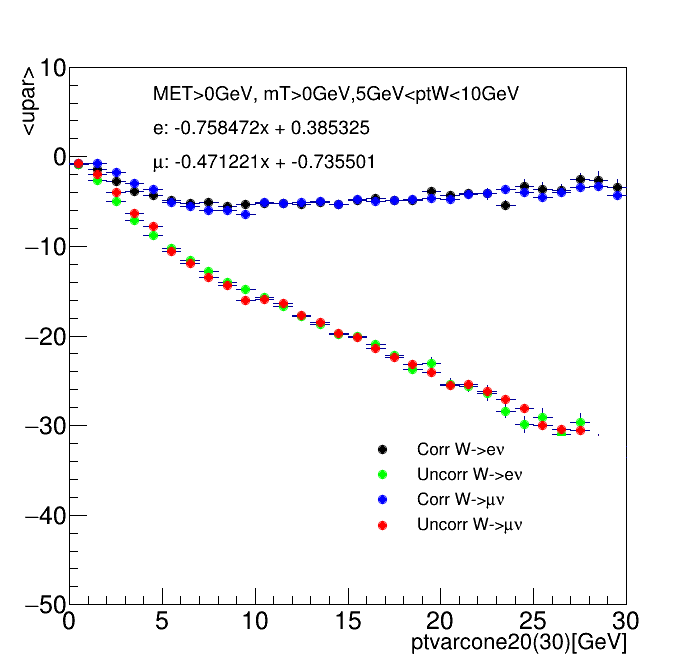
\includegraphics[width=0.32\textwidth]{bias/data/2}
 	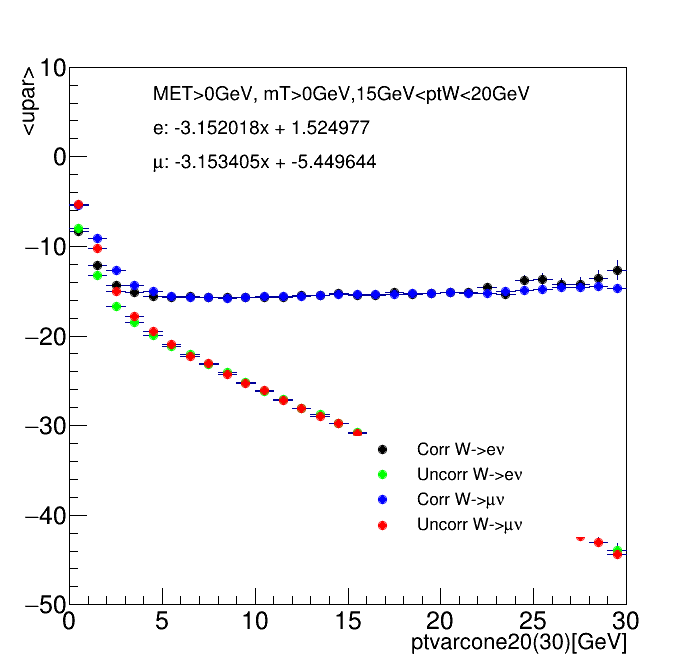
\includegraphics[width=0.32\textwidth]{bias/data/4}
 	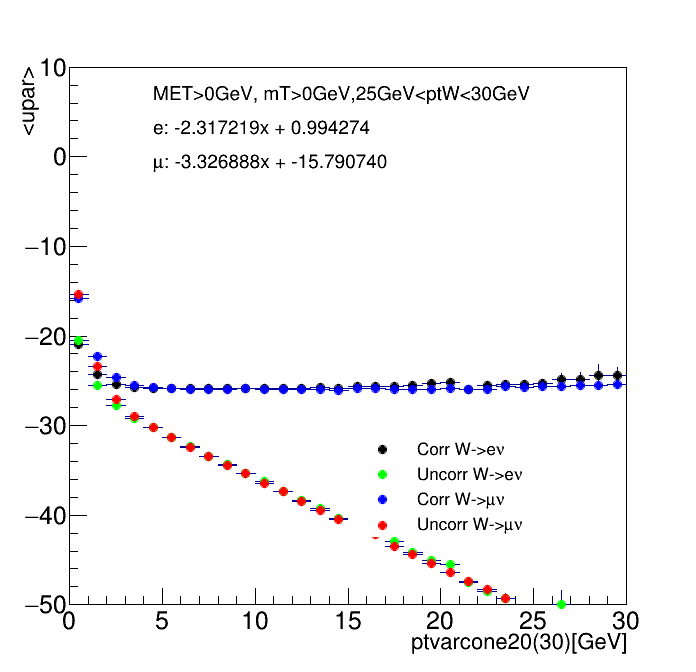
\includegraphics[width=0.32\textwidth]{bias/data/6}
 	\caption{$<u_\parallel^\ell>$ as a function of \texttt{ptcone20}, before and after correction using data samples at $\sqrt{s}$ = 13~TeV.}
 	\label{fig:calib_upar}
 \end{figure}
Some residual dependence of the extrapolated distributions on the isolation criteria is still present and requires shape extrapolation procedure. The shape of the distribution of interest is estimated in three slices of \texttt{ptvarcone20/pT} isolation within [0.10, 0.20, 0.30 0.40] in CR2. For every observable $X$ the difference $\Delta[X]$ of the distribution $X$ between consecutive isolation slices is defined as:
\begin{equation}
H_{MJ}^{[0.1,0.2]}[X] = H_{data}^{[0.1,0.2]}[X] - H_{MC}^{[0.1,0.2]}[X]; 
\end{equation}
\begin{equation}
\Delta[X]= 1/2 \left[ (H_{MJ}^{[0.1,0.2]}[X]-H_{MJ}^{[0.2,0.3]}[X]) + (H_{MJ}^{[0.2,0.3]}[X]-H_{MJ}^{[0.3,0.4]}[X]) \right],
\end{equation}
where $H_{X}^{[x,y]}$ is the normalized distribution of $X$ in CR2 (anti-isolated signal region) satisfying $x < \texttt{ptvarcone20/pT} < y$, estimated from the MC-subtracted data in CR2.\\
$\Delta[X]$ is supposed to be the difference between MJ sprectrum in the signal region (\texttt{ptvarcone20/pT}$<0.1$)  and the isolation slice next to it (0.10 < \texttt{ptvarcone20/pT} < 0.20).
So the extrapolated distribution to the signal region is the following:
\begin{equation}
H_{X}^{sig} = H_{X}^{[0.1,0.2]} - \Delta[X].
\end{equation}

The applied shift $\Delta[X]$ is assigned a 100\% relative uncertainty because of the large statistical uncertainty. Figures \ref{fig:mjbkg-elp-corr-scan} and \ref{fig:mjbkg-mup-corr-scan} contain the results of the isolation scan in electron and muon channels respectively. 

\begin{figure}[htbp]
	\centering
	\includegraphics[width=0.48\textwidth]{scan_uncalib/PTW_3/ScanFit/Wep.png}
	\includegraphics[width=0.48\textwidth]{scan_calib/PTW_3/ScanFit/Wep.png}\\
	\caption{Isolation scan in the $W^+\to e^+\nu$ channel without (left) and with (right) recoil correction~\cite{mjets_int_note_6}.}
	\label{fig:mjbkg-elp-corr-scan}
\end{figure}

\begin{figure}[htbp]
	\centering
	\includegraphics[width=0.48\textwidth]{scan_uncalib/PTW_3/ScanFit/Wmup.png}
	\includegraphics[width=0.48\textwidth]{scan_calib/PTW_3/ScanFit/Wmup.png}\\
	\caption{Isolation scan in the $W^+\to \mu^+\nu$ channel without (left) and with (right) recoil correction~\cite{mjets_int_note_6}.}
	\label{fig:mjbkg-mup-corr-scan}
\end{figure}

The MJ contributions to the kinematic distributions in slices of isolation along with the extrapolation to the signal region for the 13 TeV for electrons and muons are shown in Figures \ref{fig:mjbkg-shape-lep} and \ref{fig:mjbkg-shape}. The kinematic distributions with the contributions from the multijets for 5 and 13 TeV are presented in sections \ref{subsec:controlplots5} and \ref{subsec:controlplots13} respectively.
\begin{figure}[htbp]
	\centering
	\includegraphics[width=0.48\textwidth]{plot_ratio_isoslice/PTW_3/CR_2_calib/Wep/leppt.png}
	\includegraphics[width=0.48\textwidth]{plot_ratio_isoslice/PTW_3/CR_2_calib/Wmup/leppt.png}\\
	\caption{Extrapolation of the multijet distributions for the lepton transverse momentum in the $W^+\to e^+\nu$ (left) and $W^+\to \mu^+\nu$ (right) channels at $\sqrt{s}=13$~TeV~\cite{mjets_int_note_6}.}
	\label{fig:mjbkg-shape-lep}
\end{figure}

\begin{figure}[htbp]
	\includegraphics[width=0.48\textwidth]{plot_ratio_isoslice/PTW_3/CR_2_calib/Wep/pfo_met.png}
	\includegraphics[width=0.48\textwidth]{plot_ratio_isoslice/PTW_3/CR_2_calib/Wmup/pfo_met.png}\\
	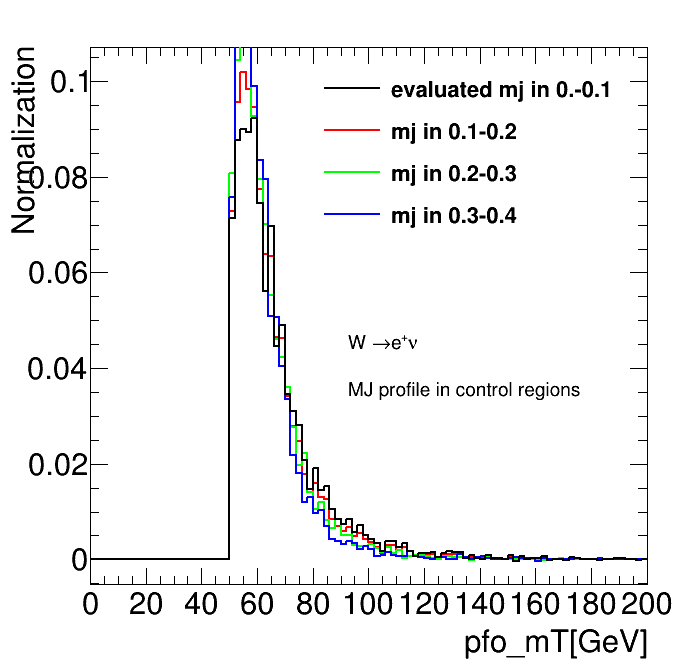
\includegraphics[width=0.48\textwidth]{plot_ratio_isoslice/PTW_3/CR_2_calib/Wmup/pfo_mT.png}
	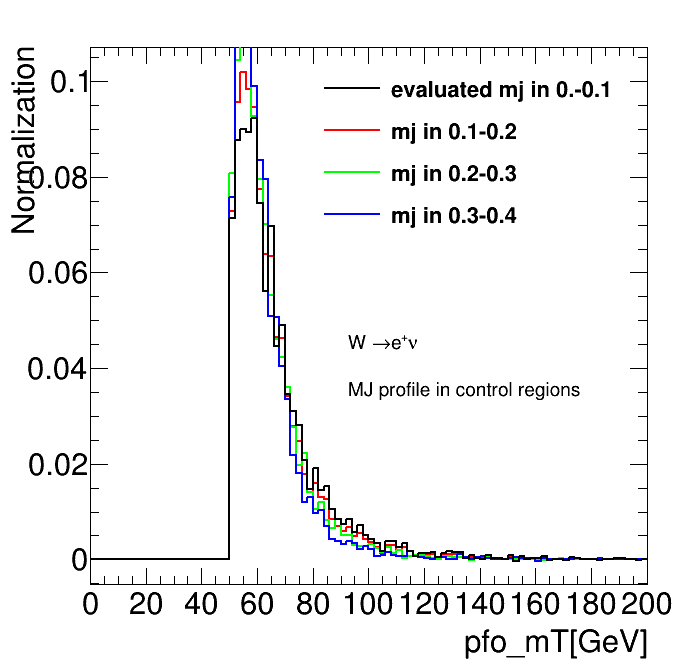
\includegraphics[width=0.48\textwidth]{plot_ratio_isoslice/PTW_3/CR_2_calib/Wmup/pfo_mT.png}\\
	\caption{Extrapolation of the multijet distributions for the missing transverse energy (top) and transverse mass (bottom), in the $W^+\to e^+\nu$ (left) and $W^+\to \mu^+\nu$ (right) channels at $\sqrt{s}=13$~TeV~\cite{mjets_int_note_6}.}
	\label{fig:mjbkg-shape}
\end{figure}
The multijet yields for all channels and energies are presented in Table \ref{table:mj_summary} along with the associated uncertainties. The table shows that the MJ background is significantly higher in the electron channel than in the muon channel. 
\begin{table}[h!]
	\begin{center}
		\begin{tabular}{|c|c|c|}
			\hline
			Channel & 13 TeV & 5 TeV \\
			\hline
			$W^+\to e^{+}\nu$ & 27973 $\pm$ 1756 &  3027 $\pm$ 554 \\
			$W^+\to e^{-}\nu$ & 27388 $\pm$ 1962 &  2401 $\pm$ 495 \\
			$W^+\to \mu^{+}\nu$ & 9044 $\pm$ 796 &  724 $\pm$ 192 \\
			$W^+\to \mu^{-}\nu$ & 9053 $\pm$ 617 & 755 $\pm$ 160 \\
			\hline
		\end{tabular}
		\caption{Evalution of multijet background yields at 13~TeV and 5~TeV~\cite{mjets_int_note_6}.}
		\label{table:mj_summary}
	\end{center}
\end{table}
\clearpage
     \section{Z vertex reweighting }
The 5 TeV MC samples have been generated to be perfectly matched to the data 
Although this is not the case for 13 TeV samples, which can be seen at Fig. \ref{fig:zvtx}. 
It is also seen from these plots that the 2017 and 2018 data were collected at two different runs under different beam conditions. 
To avoid possible impact on the acceptance the MC samples were reweighted to the data using \Zee and \Zmm selections. Throughout the analysis the data collected at 13 TeV during the two runs in 2017 and 2018 are used in a combination. For this reason the correction for the MC is obtained from the combination of the two datasets (see Fig. \ref{fig:zvtx}).  

\begin{figure}[tph]
	\centering
	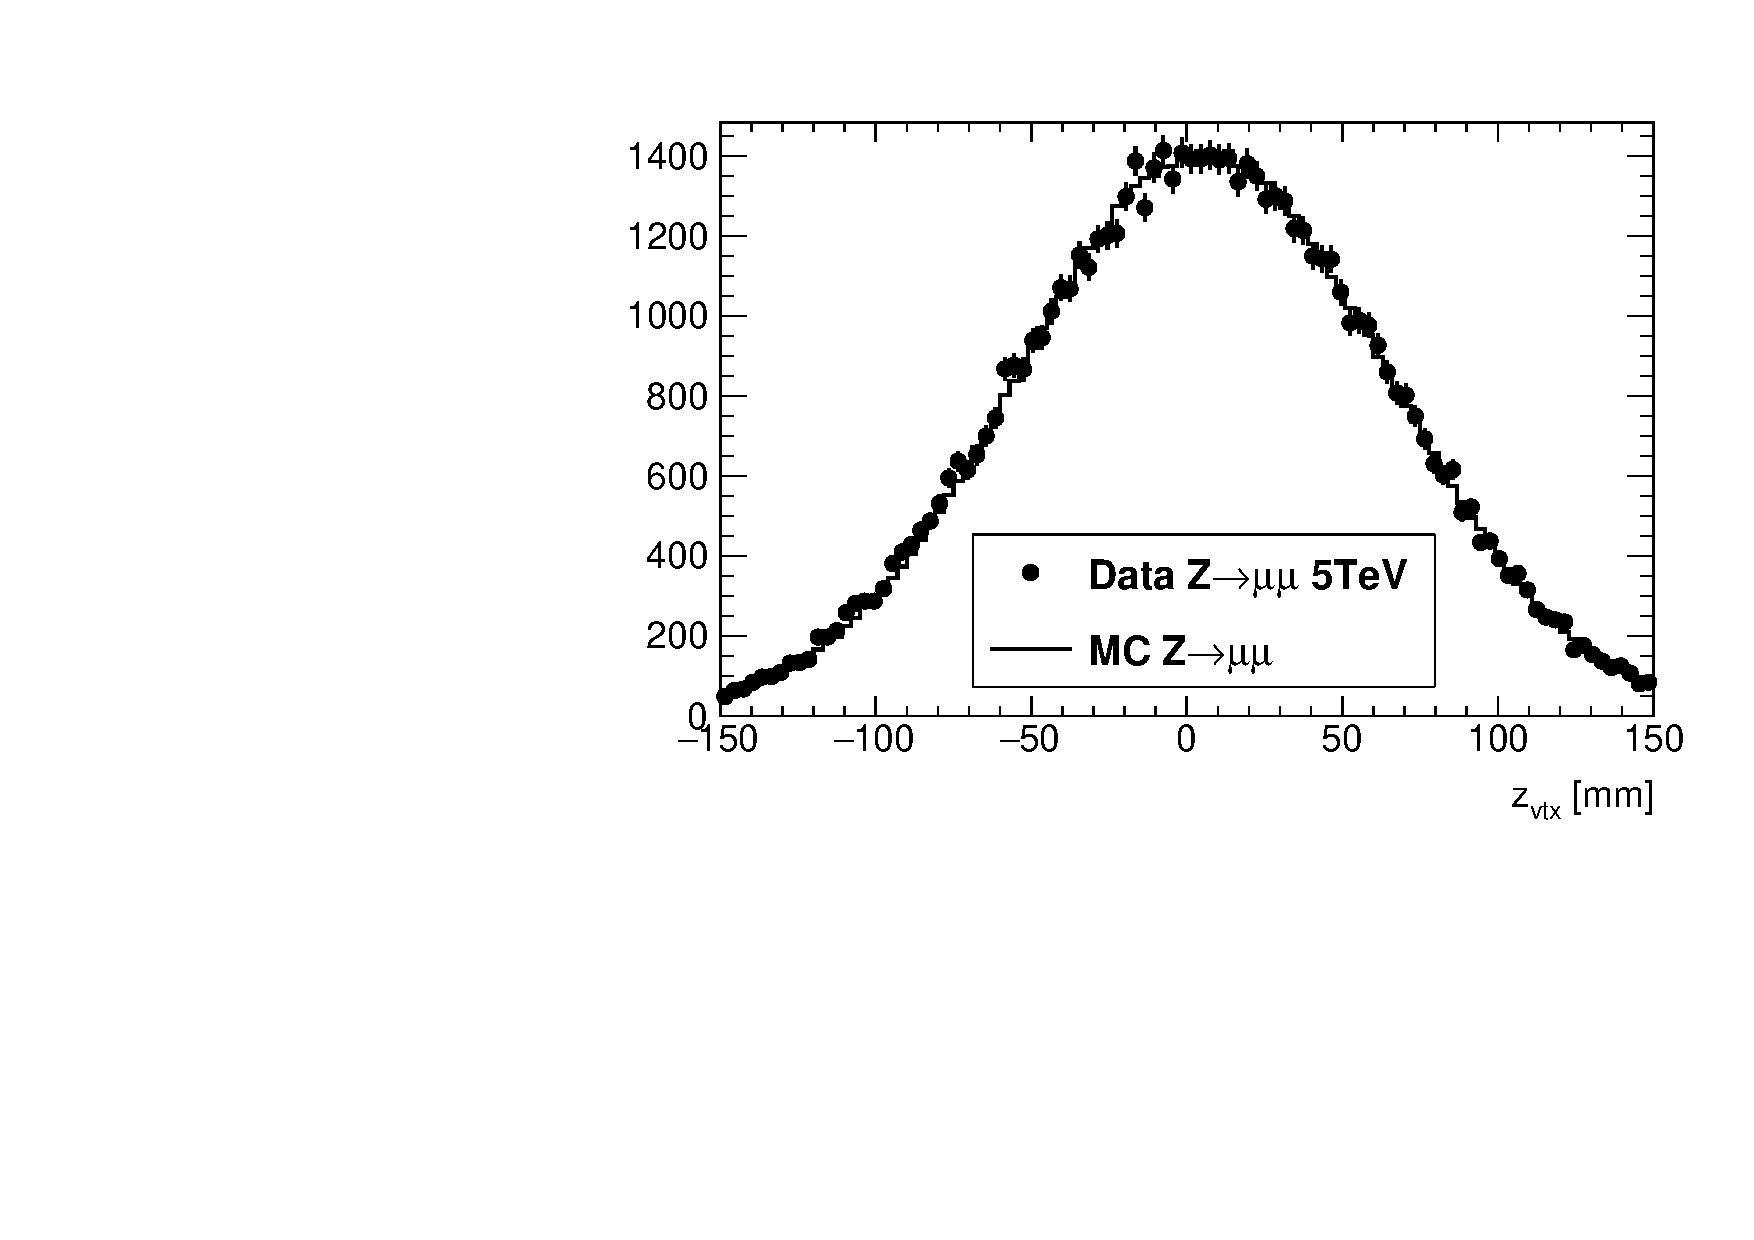
\includegraphics[width=.5\textwidth]{zmumu_5tev_zvtx}%
	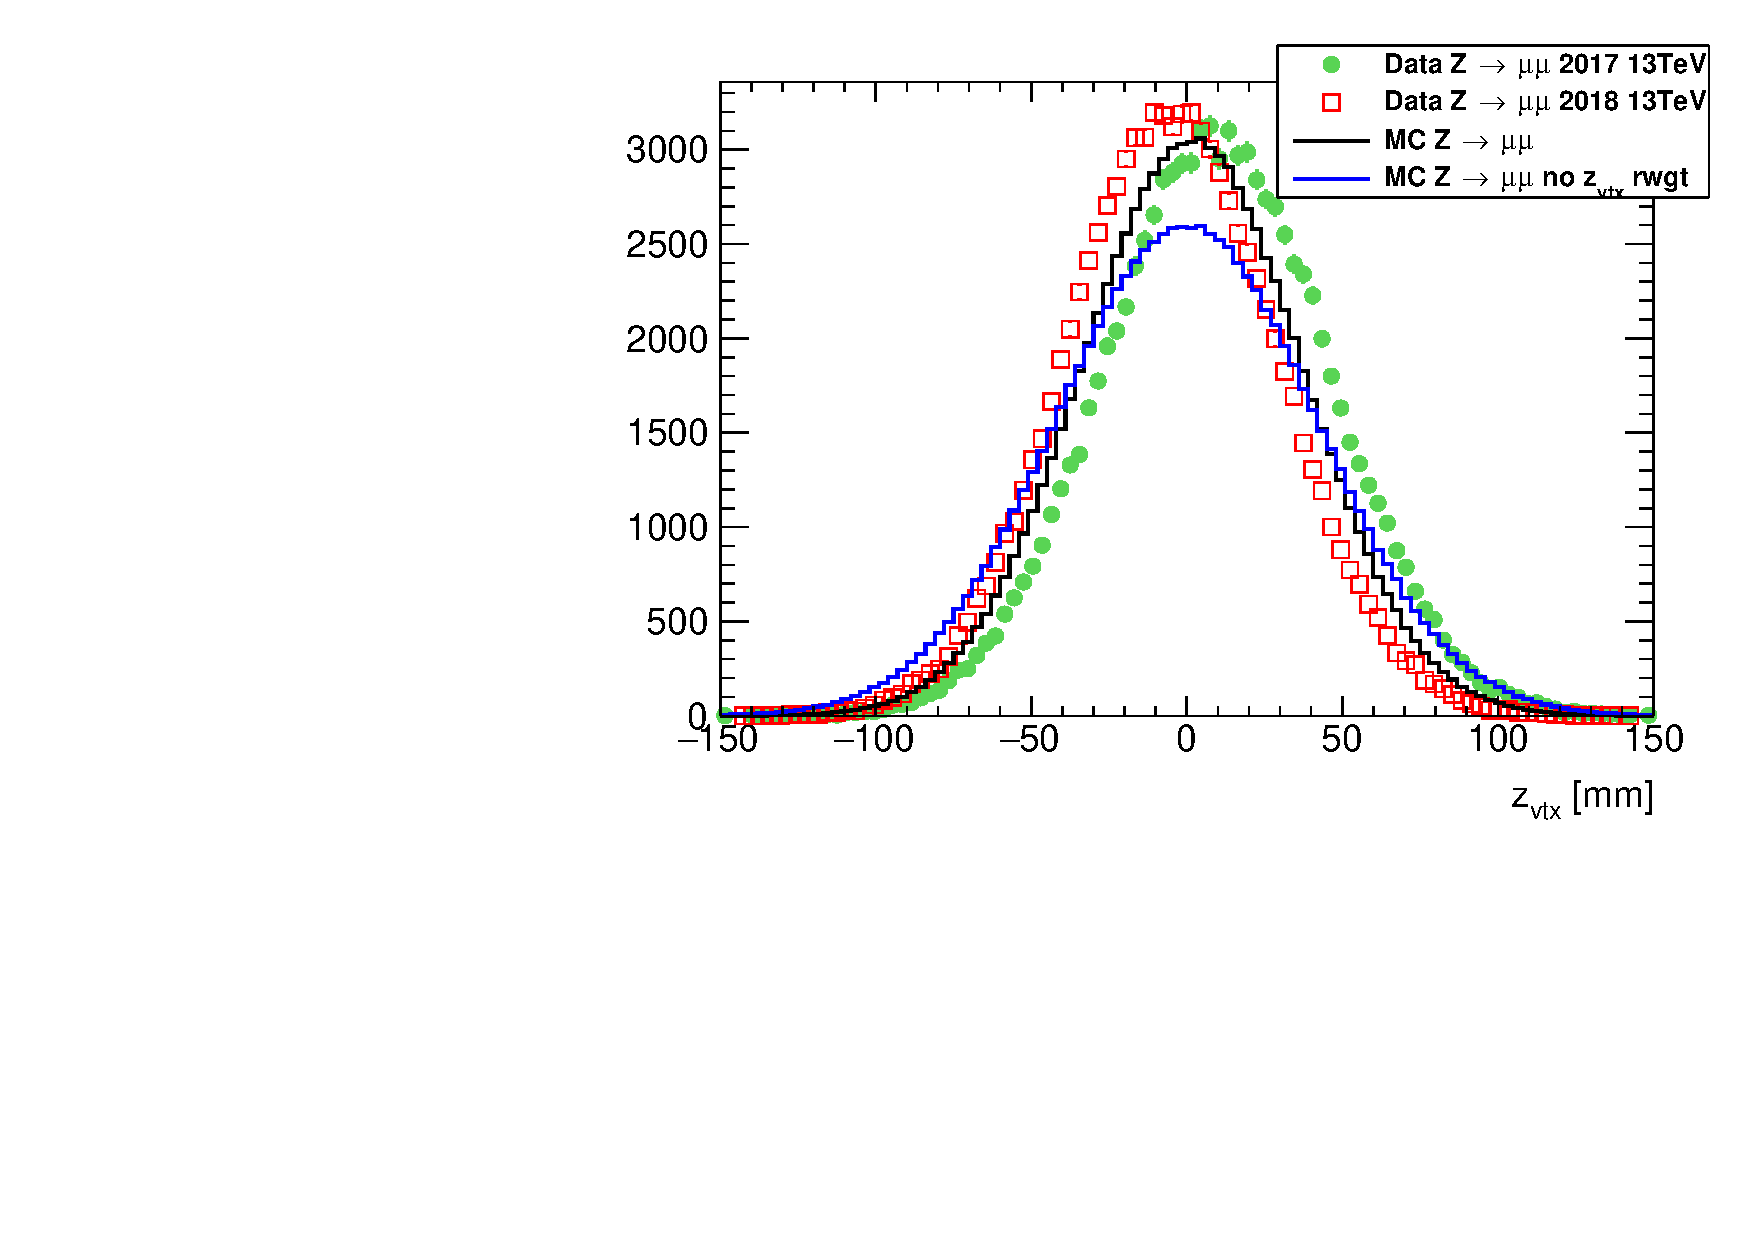
\includegraphics[width=.5\textwidth]{zmumu_13tev_zvtx_norwgt}
	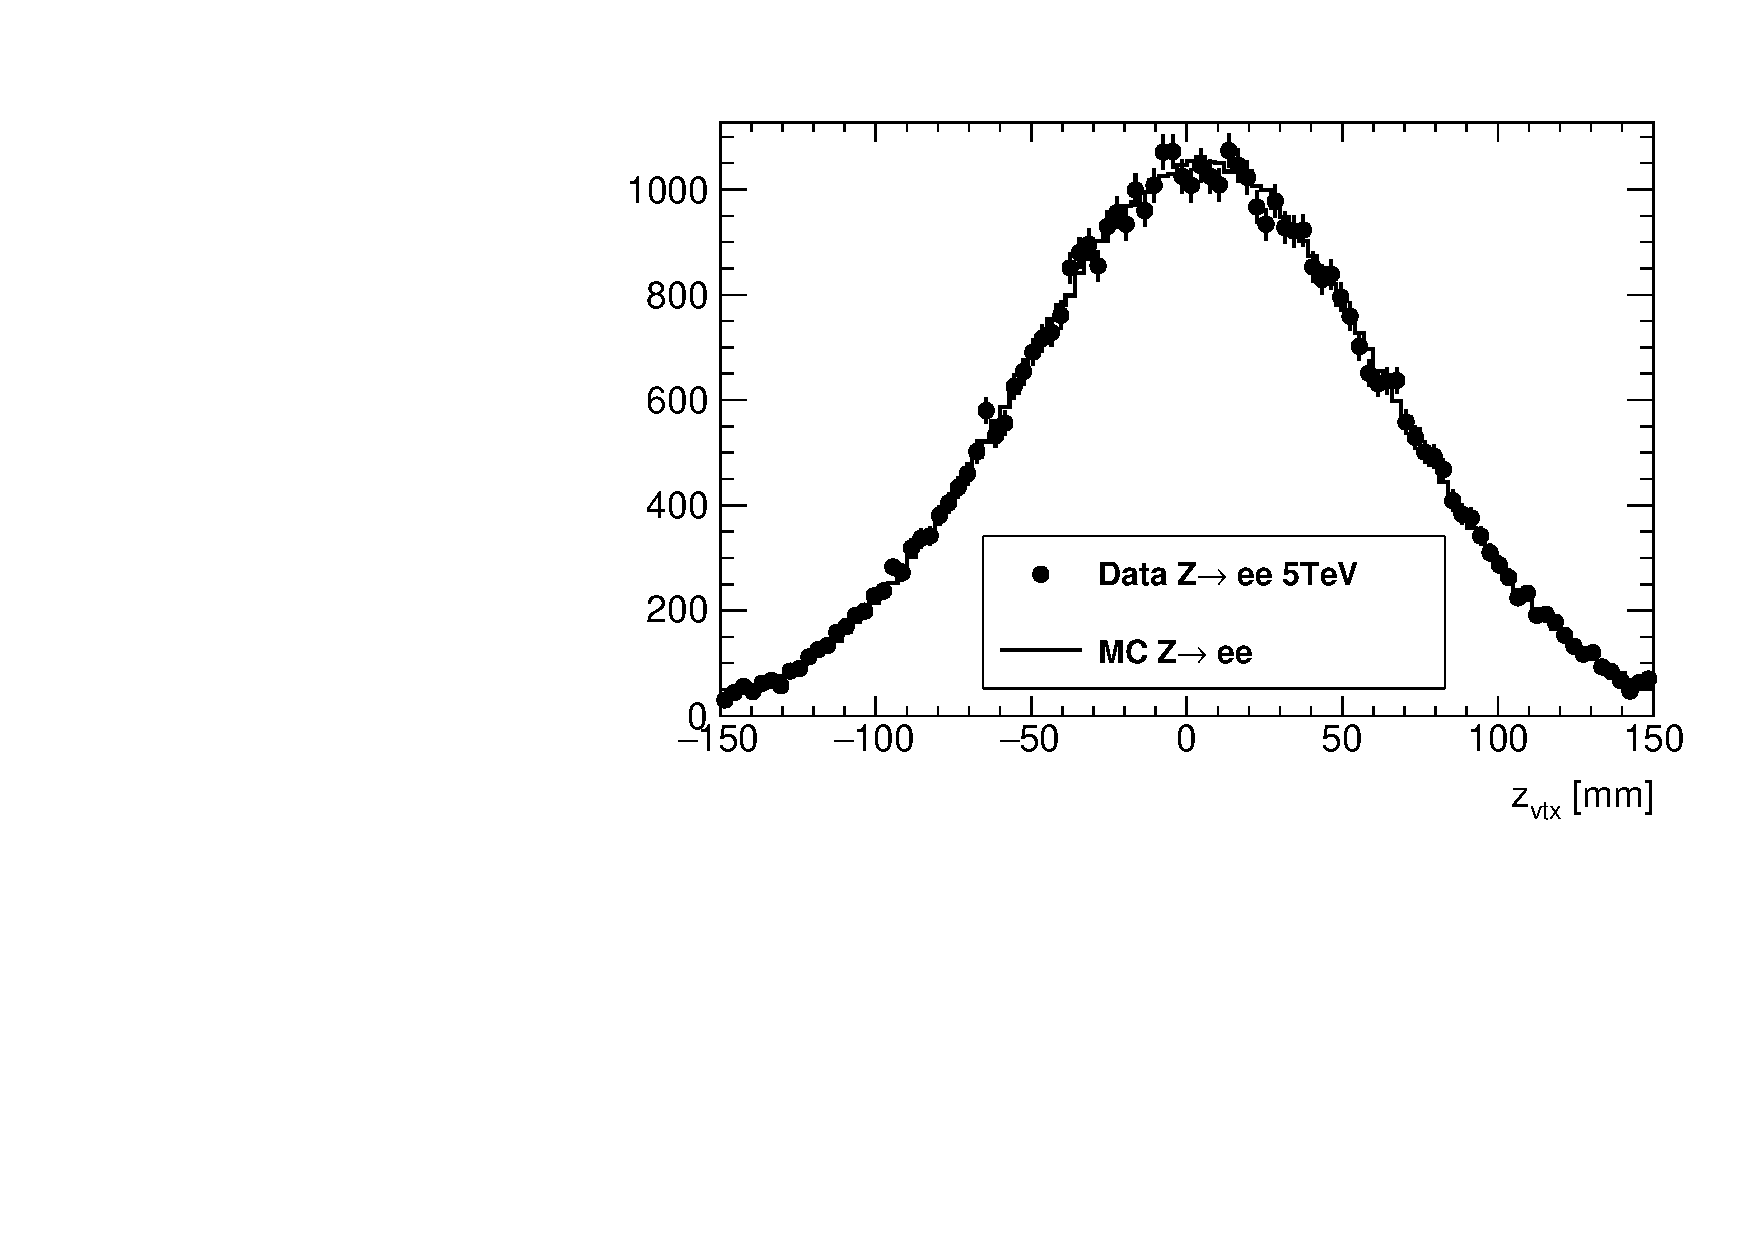
\includegraphics[width=.5\textwidth]{zee_5tev_zvtx}%
	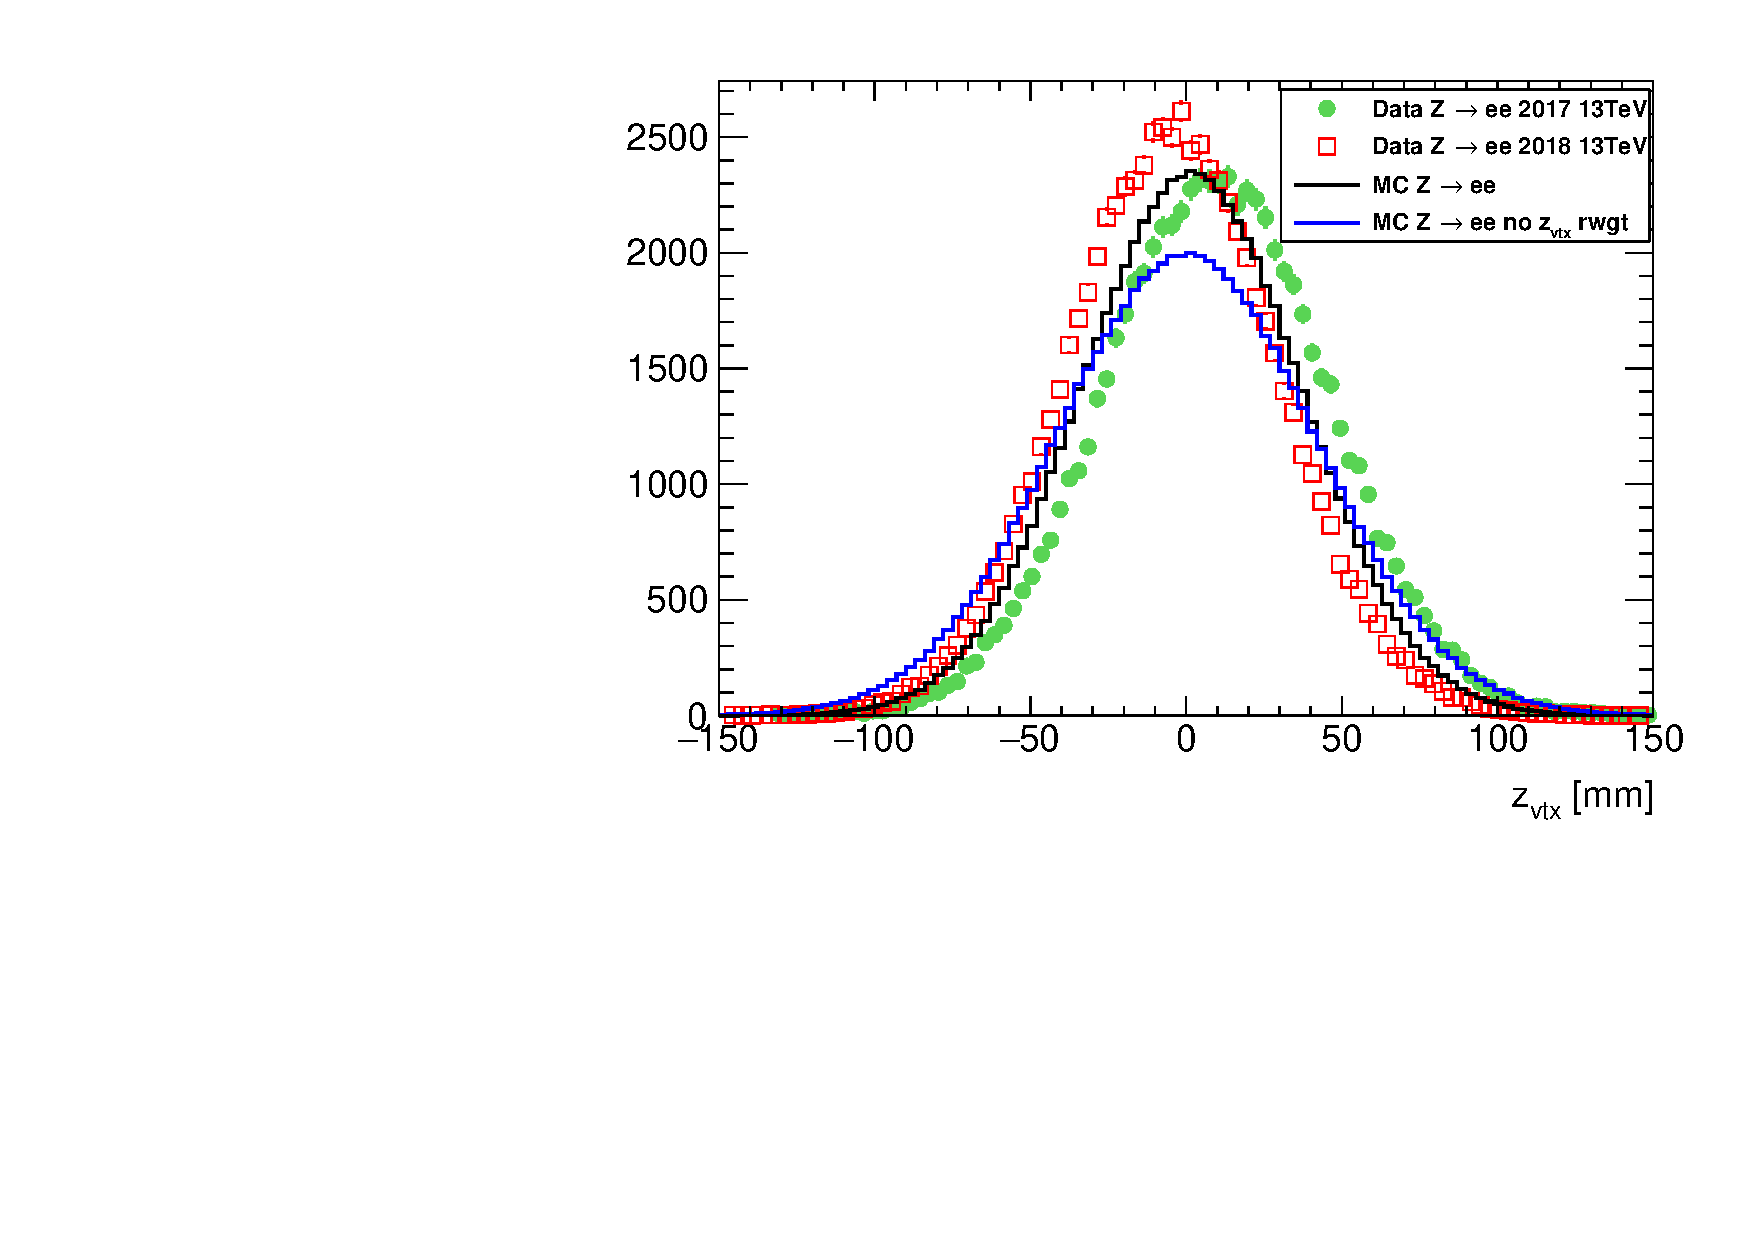
\includegraphics[width=.5\textwidth]{zee_13tev_zvtx_norwgt}
	\caption{Distributions for the 5 \TeV{} (left) and 13 \TeV{} (right)
		low-$\mu$ dataset(s) in a \Zgmm (top row) and a \Zgee (bottom row)
		selection. The data (points) is compared to \Zgmm or \Zgee signal
		MC, respectively. The distributions of the $z$-position of the
		primary vertex selected as the hard interaction are compared for
		the dataset(s) and the MC simulation before (``no $z_\mathrm{vtx}$
		rwgt'', blue, only 13 \TeV{}) and after reweighting (black). For
		the 13 \TeV{} data the 2017 and 2018 data are shown separately and
		all distributions are (roughly) normalised to the same number of
		selected events in the 2017 dataset~\cite{int_note_samples}.}
	\label{fig:zvtx}
\end{figure}

The reweighting derived from Z events is also used for the W MC samples events. The plots shown on Fig. \ref{fig:wzvtx} demonstrate that the correction derived from the Z events works well for all the W channels.  
\begin{figure}[tph]
	\centering
	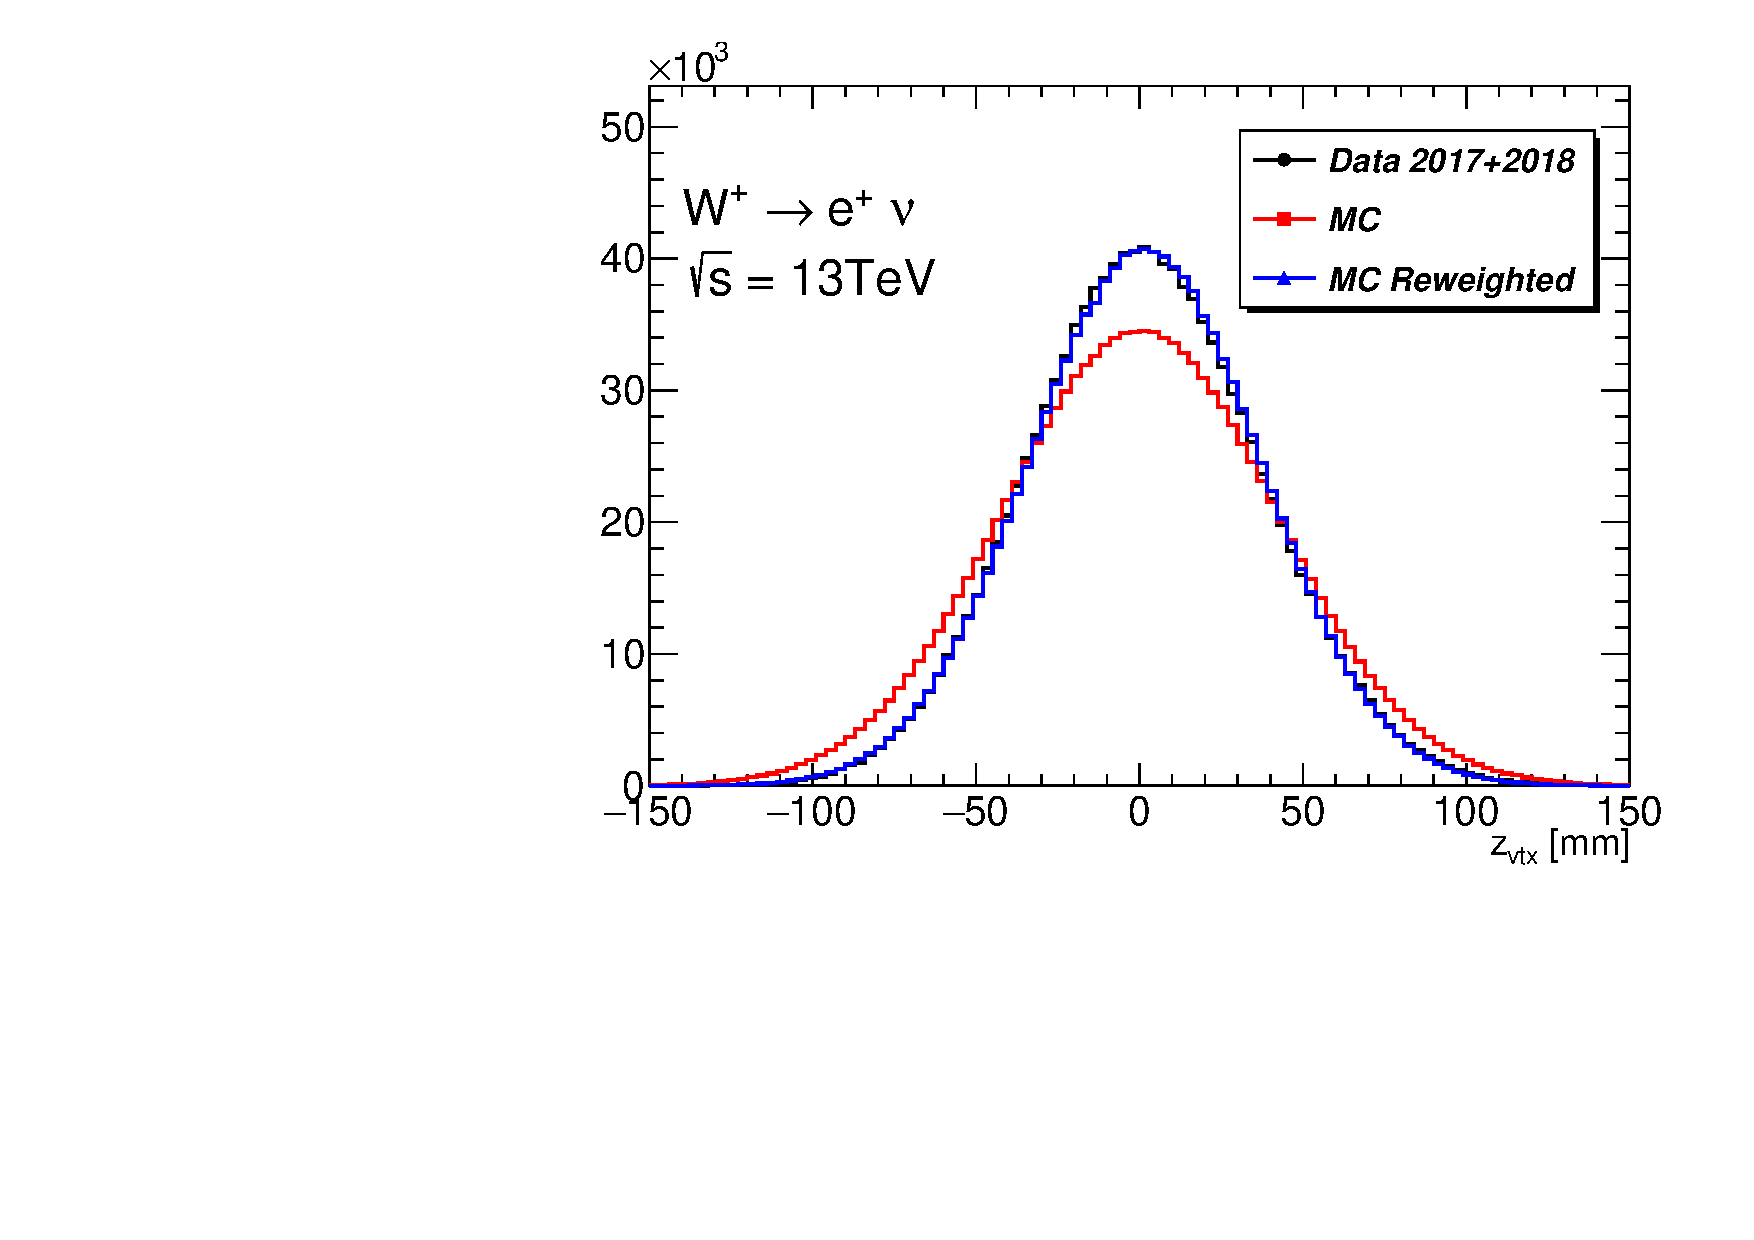
\includegraphics[width=.5\textwidth]{plusenu}%
	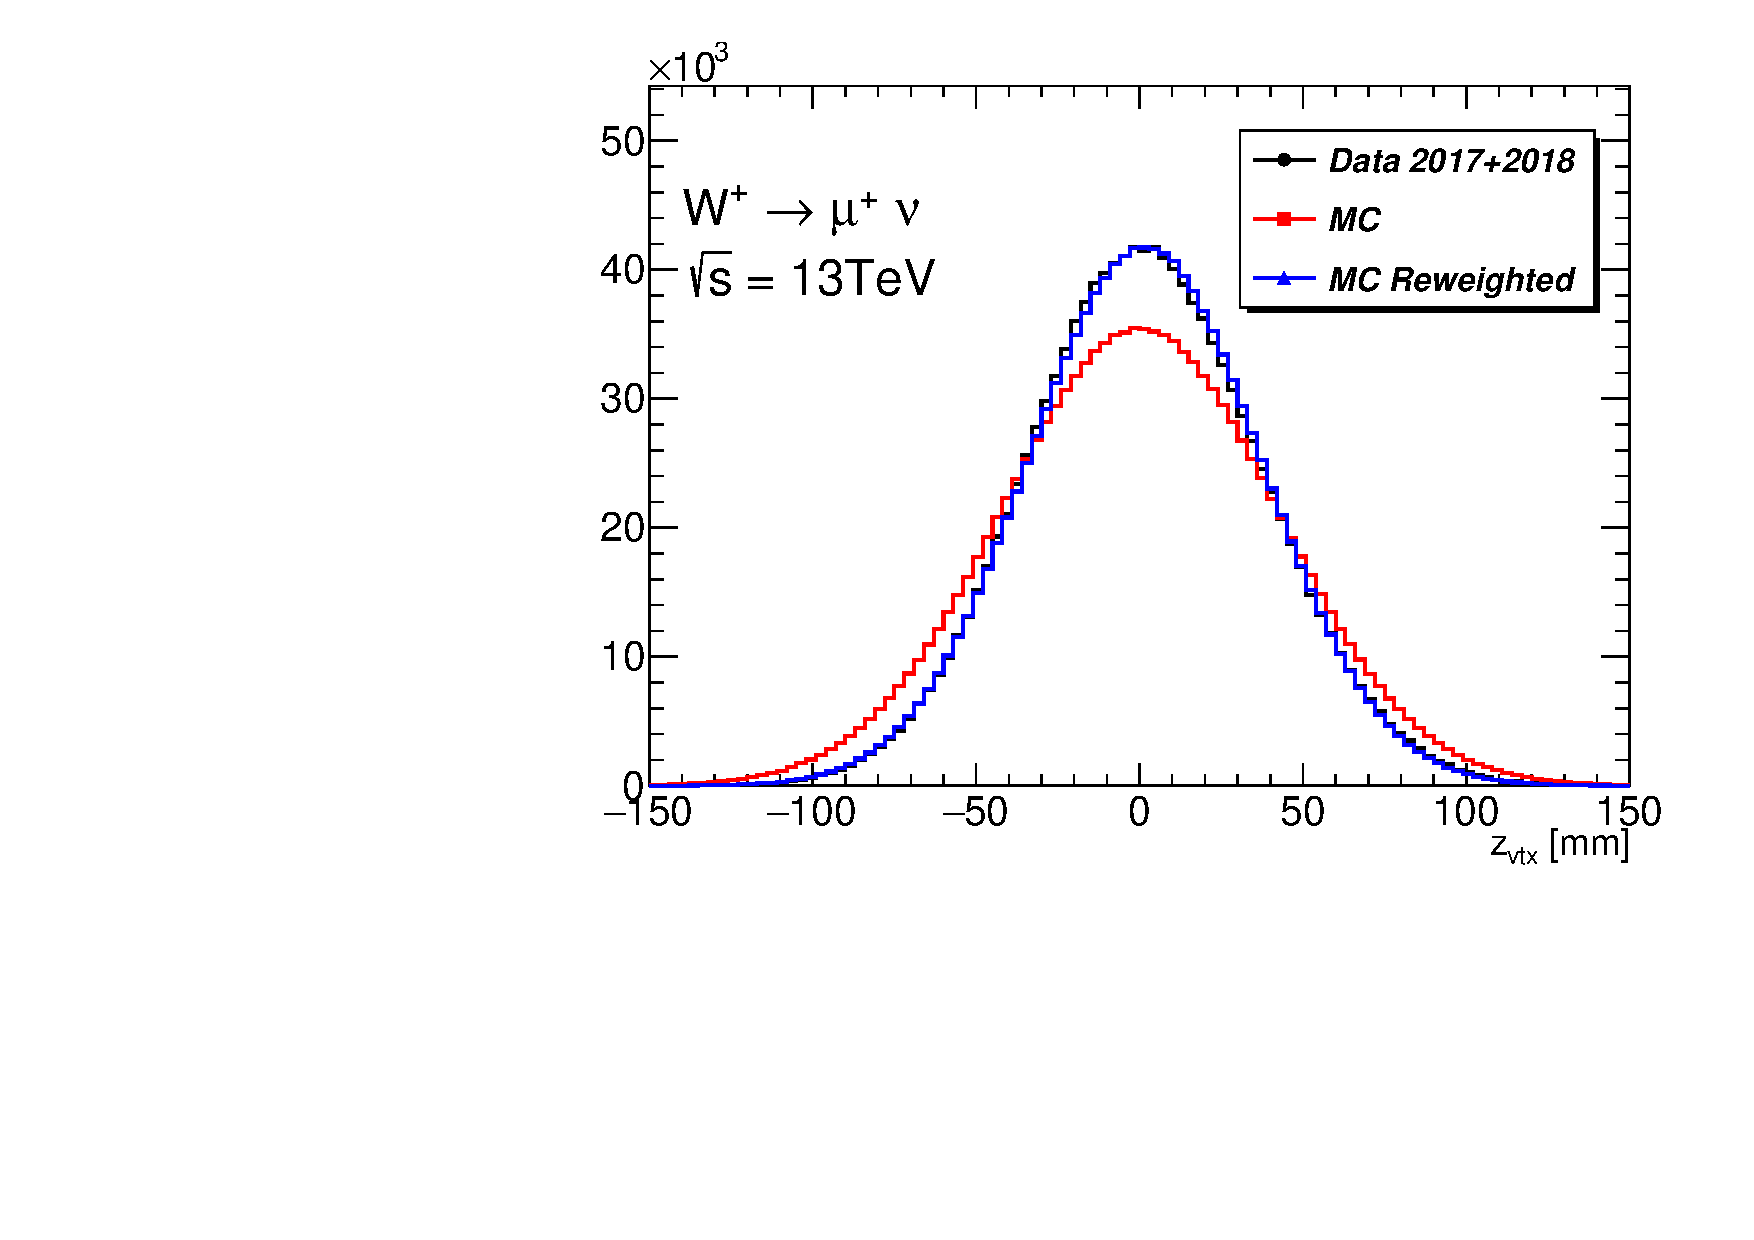
\includegraphics[width=.5\textwidth]{plusmunu}
	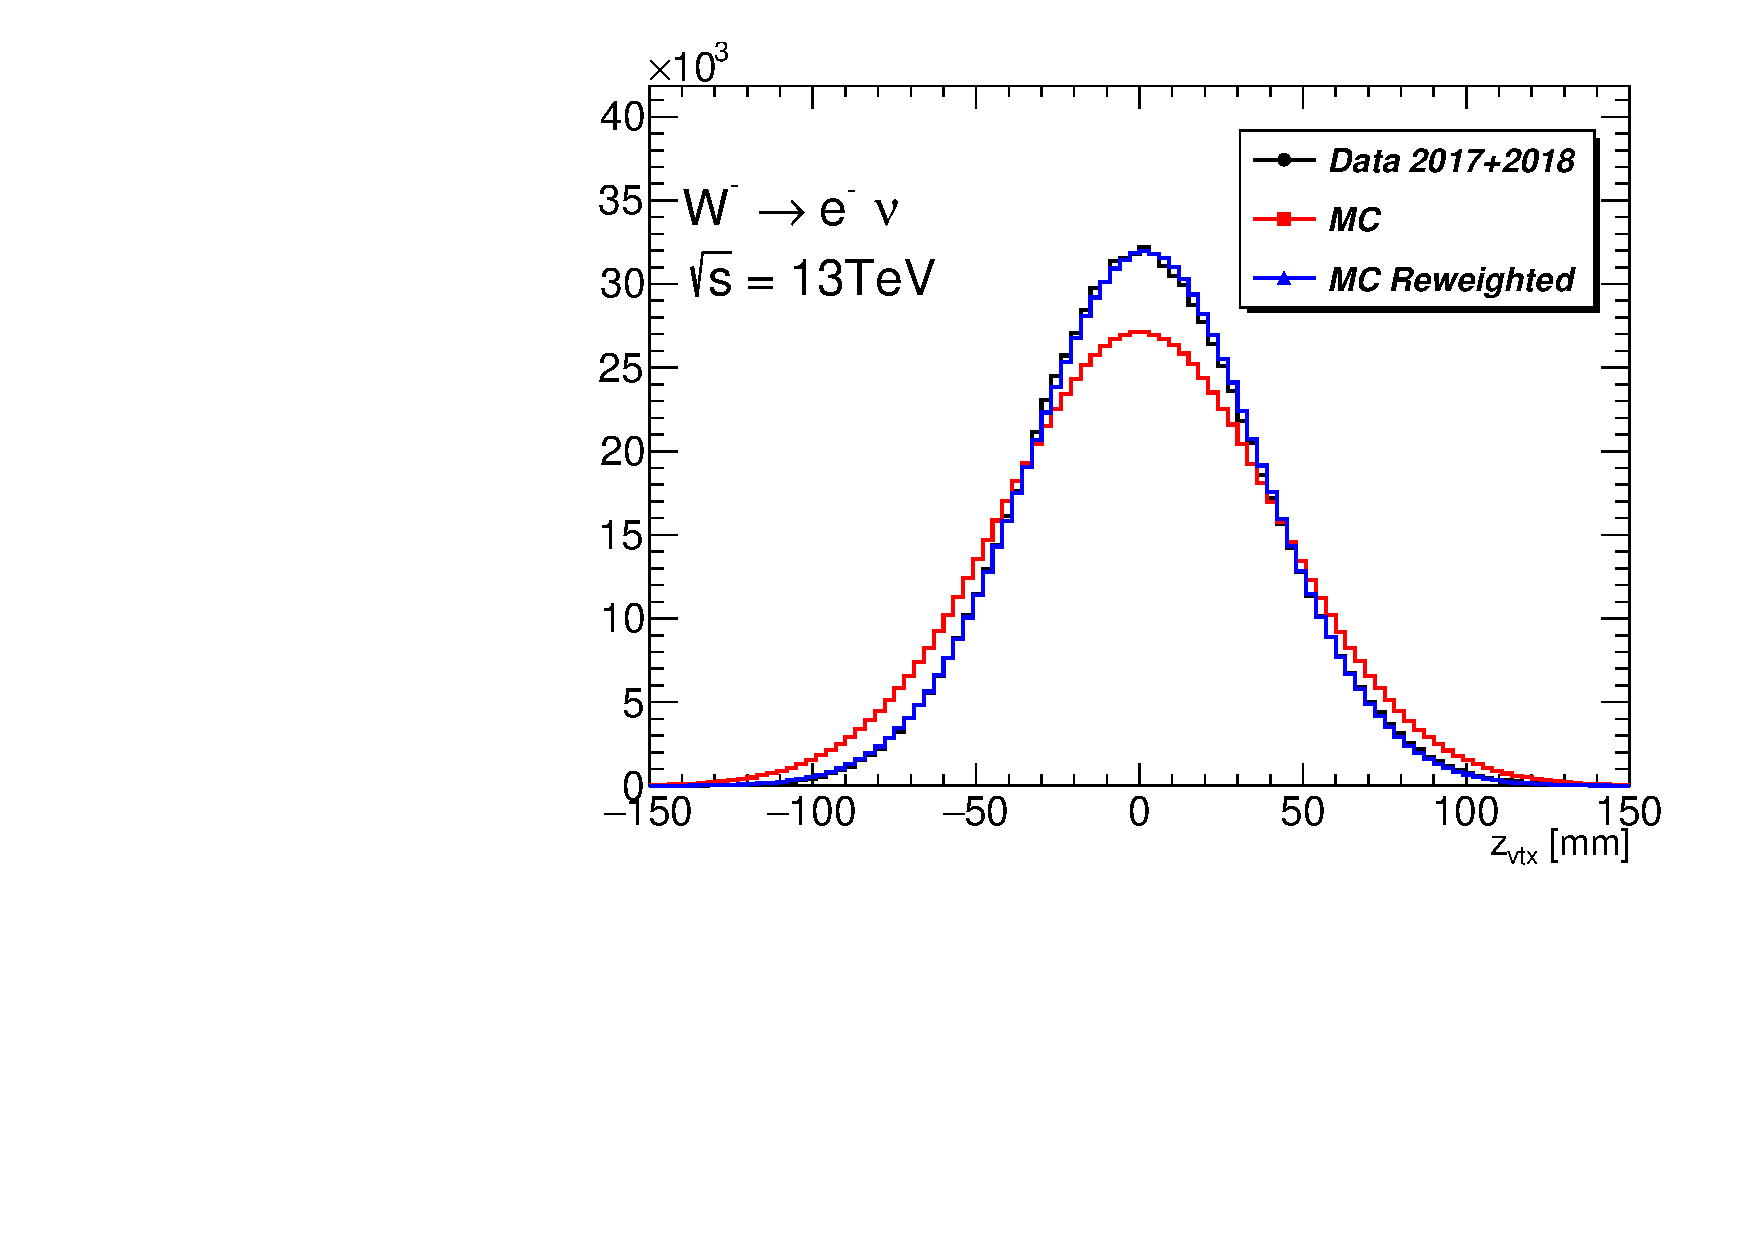
\includegraphics[width=.5\textwidth]{minusenu}%
	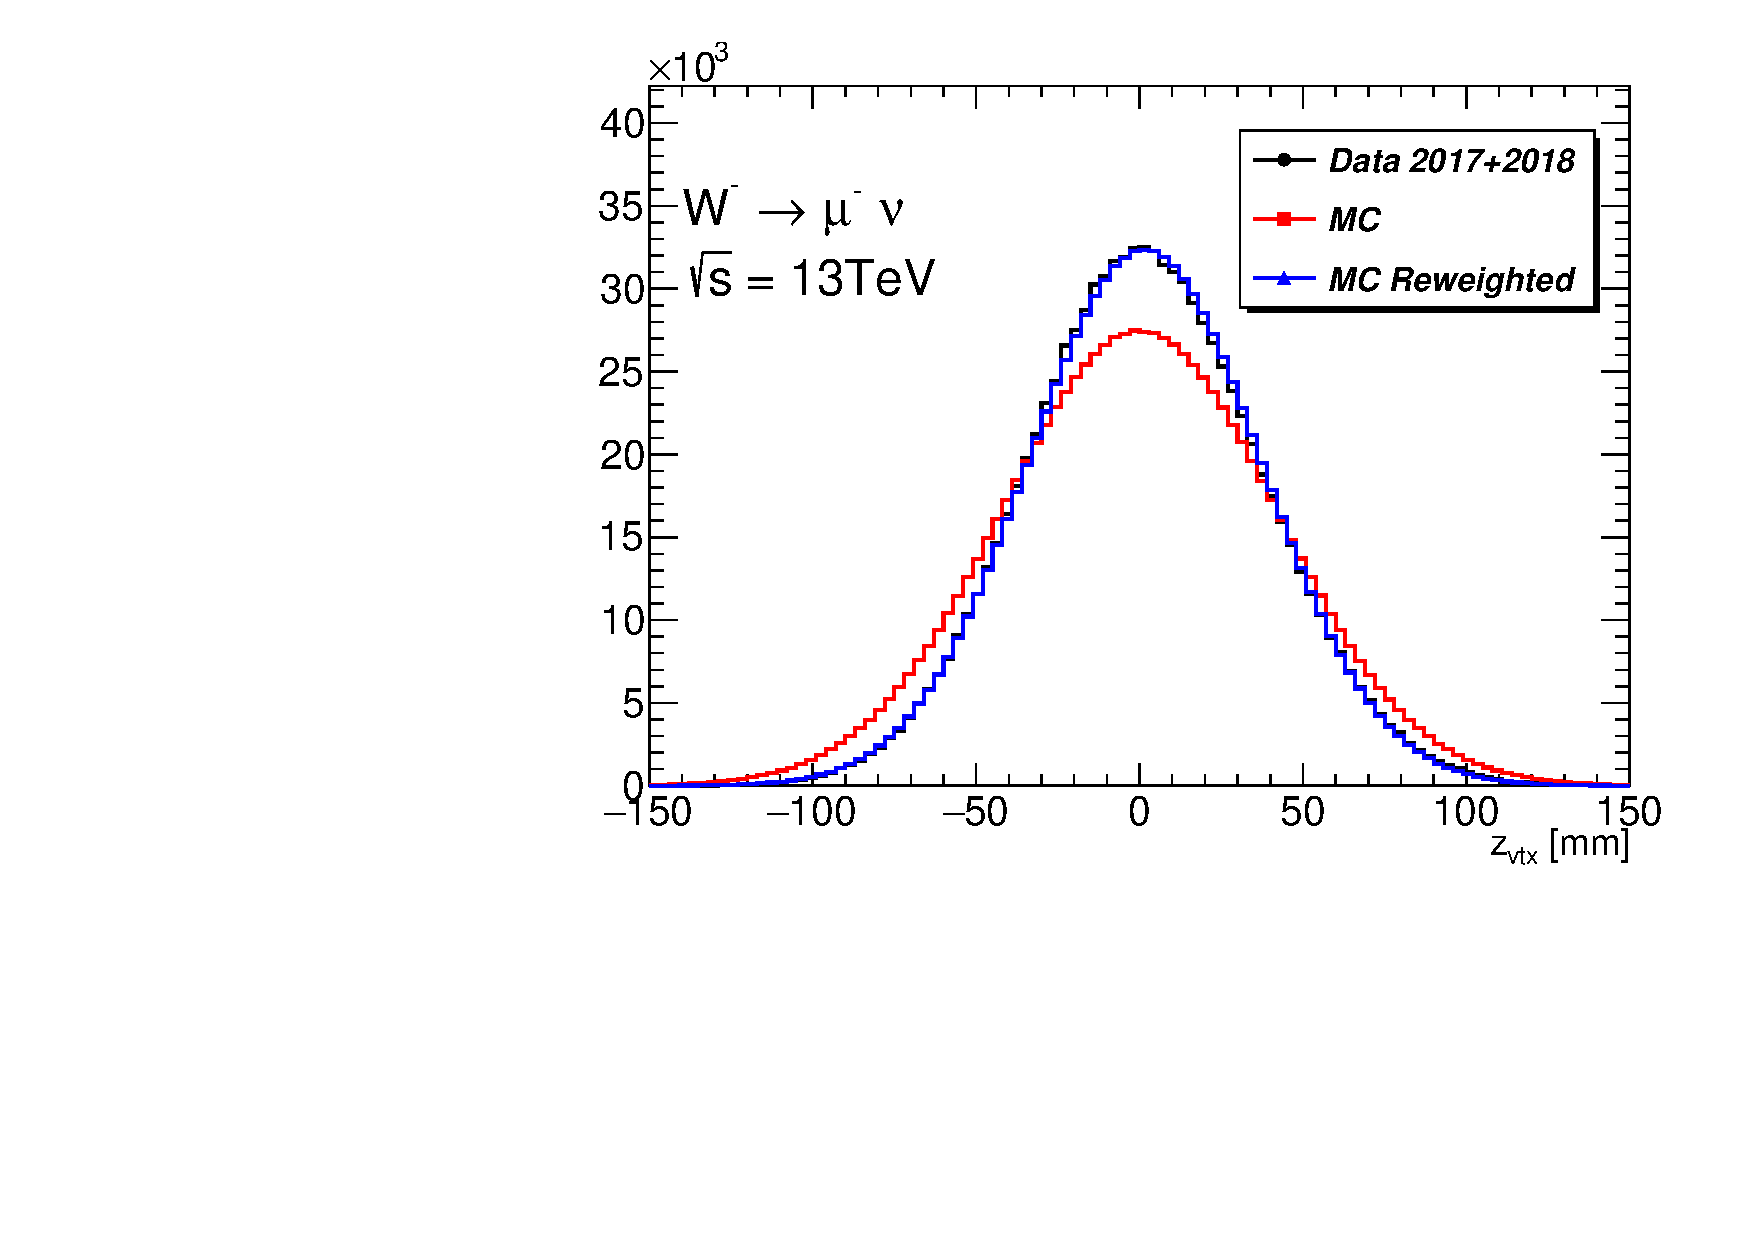
\includegraphics[width=.5\textwidth]{minusmunu}
	\caption{Distributions for 13 \TeV{} 
		low-$\mu$ dataset(s) in a $W^{+}$ (top row) and a $W^{-}$ (bottom row)
		selection in electron (left) and muon (right) channels. The combined 2017 and 2018 data (black) is compared to W MC signal before (red) and after (blue) the reweighting.
		All distributions are normalised to the same number of
		selected events in 2017+2018 dataset~\cite{int_note_samples}.}
	\label{fig:wzvtx}
\end{figure}

The reweighting causes minor effect on the kinematic distributions. The ratios of these distributions before and after the Z vertex reweighting are demonstrated for the  $W^{+}\rightarrow \mu\nu$ channel in Fig. \ref{fig:observables_wzvtx}. 

\begin{figure}[tph]
	\centering
	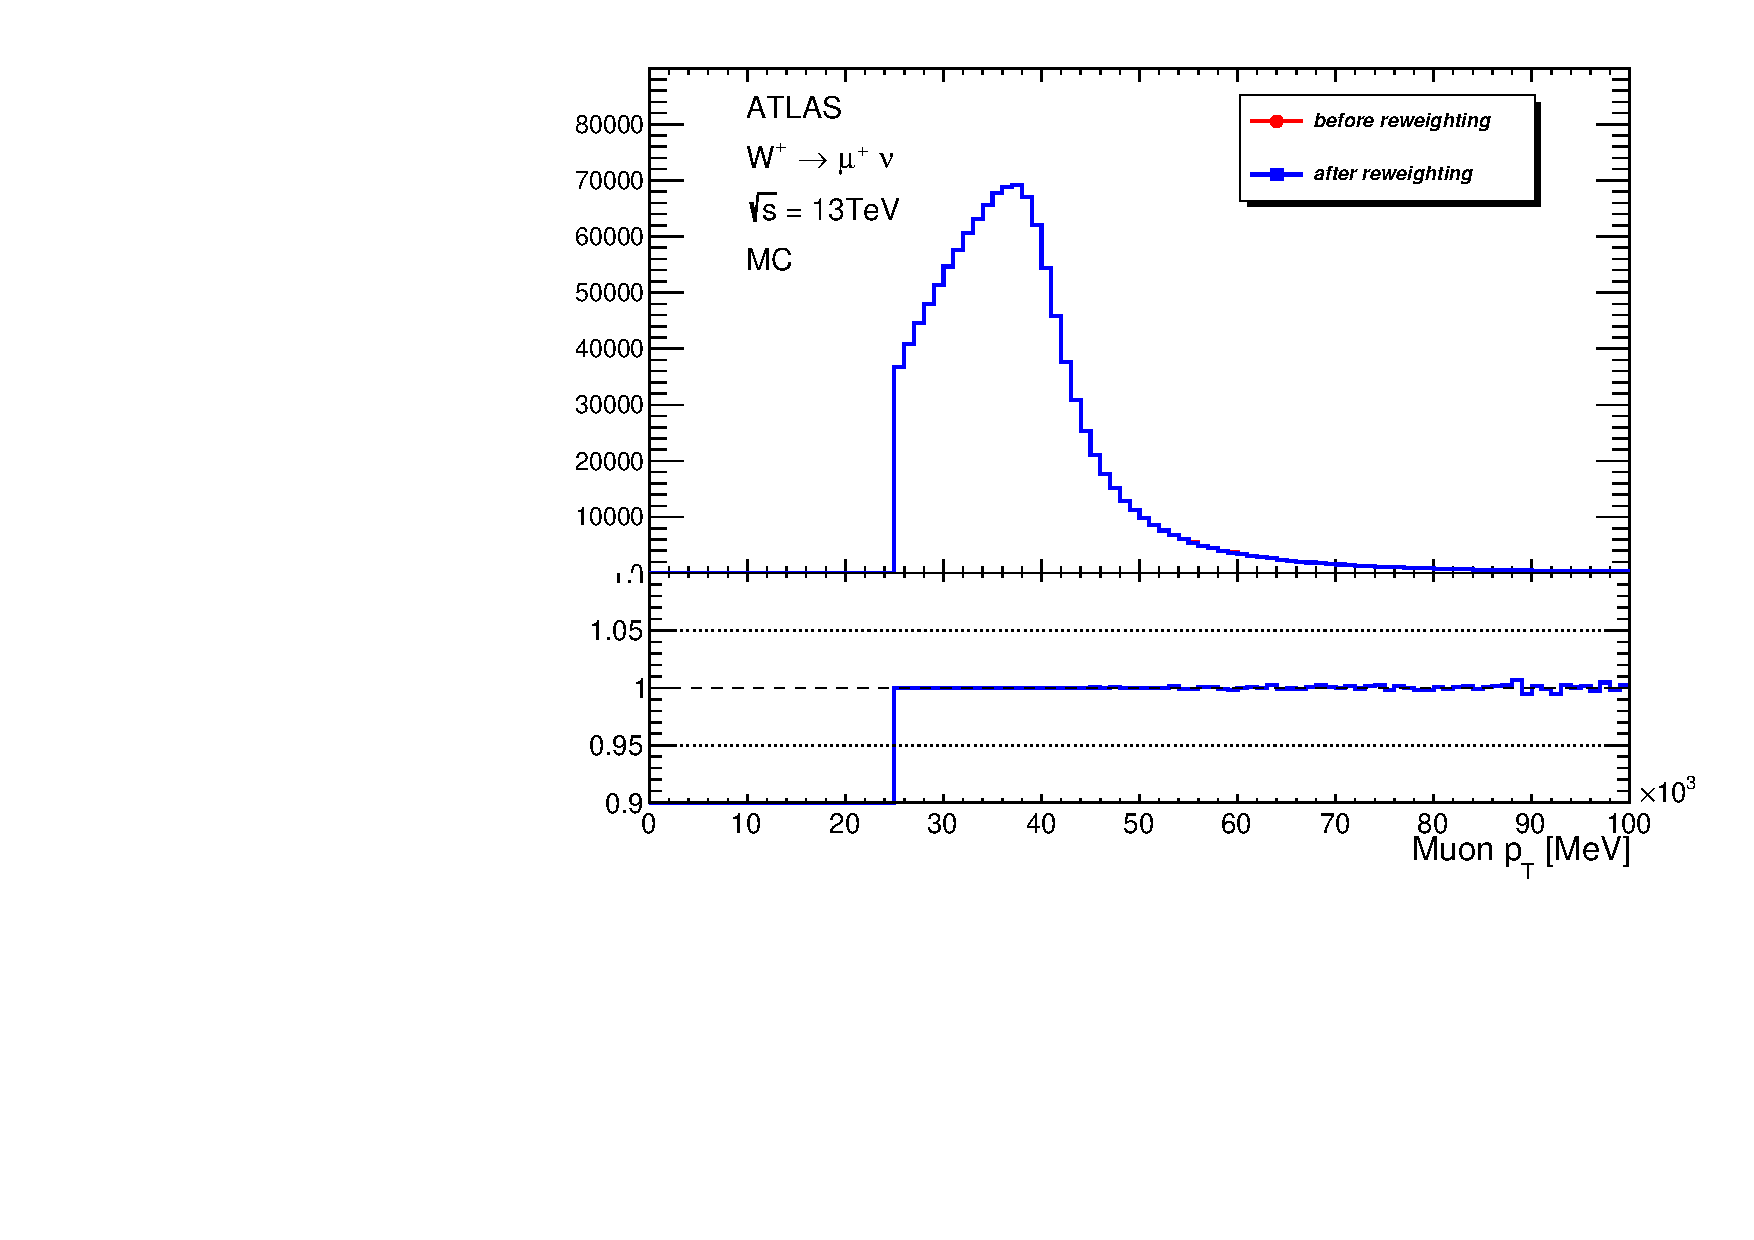
\includegraphics[width=.5\textwidth]{MC_plusmunu_WlPt_cut7_13TeV_0404_0708.pdf}%
	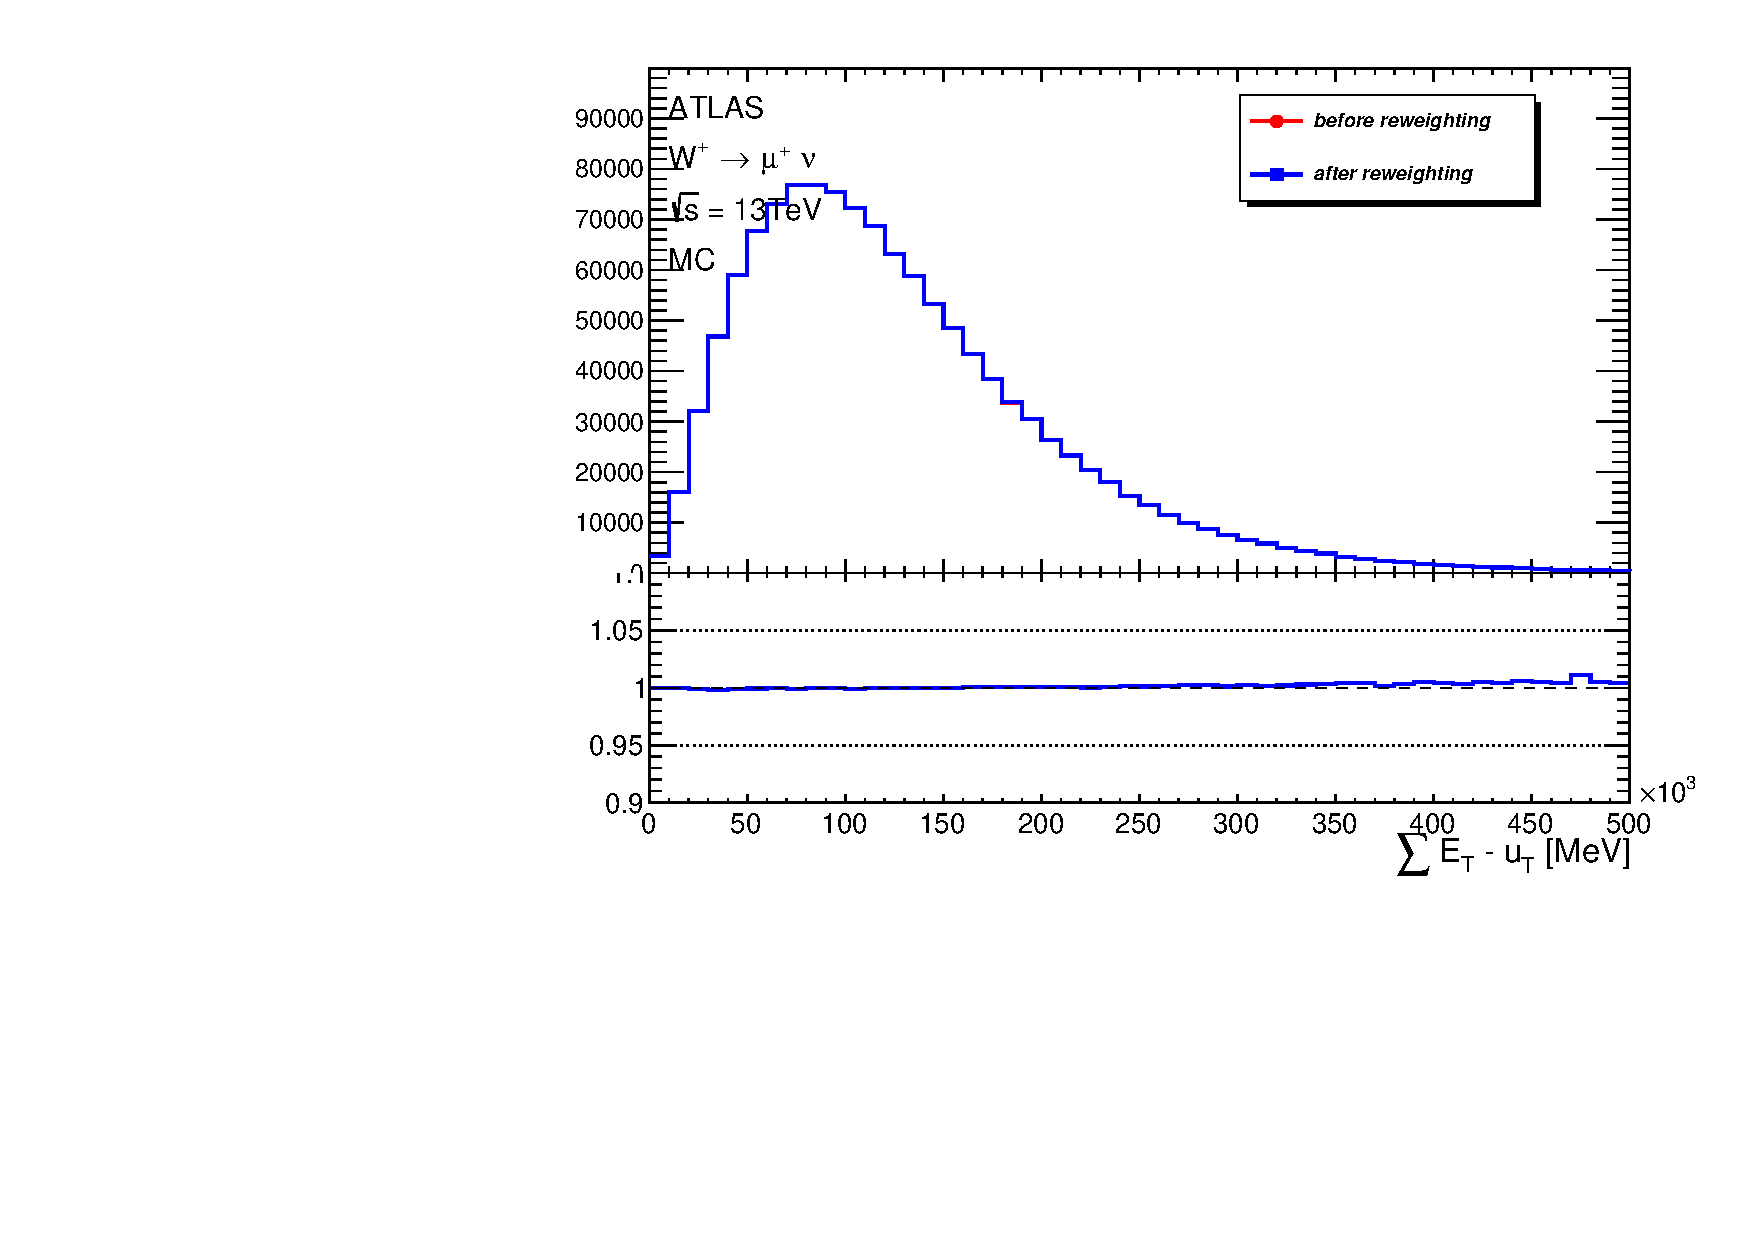
\includegraphics[width=.5\textwidth]{MC_plusmunu_WSETUE_cut7_13TeV_0404_0708.pdf}
	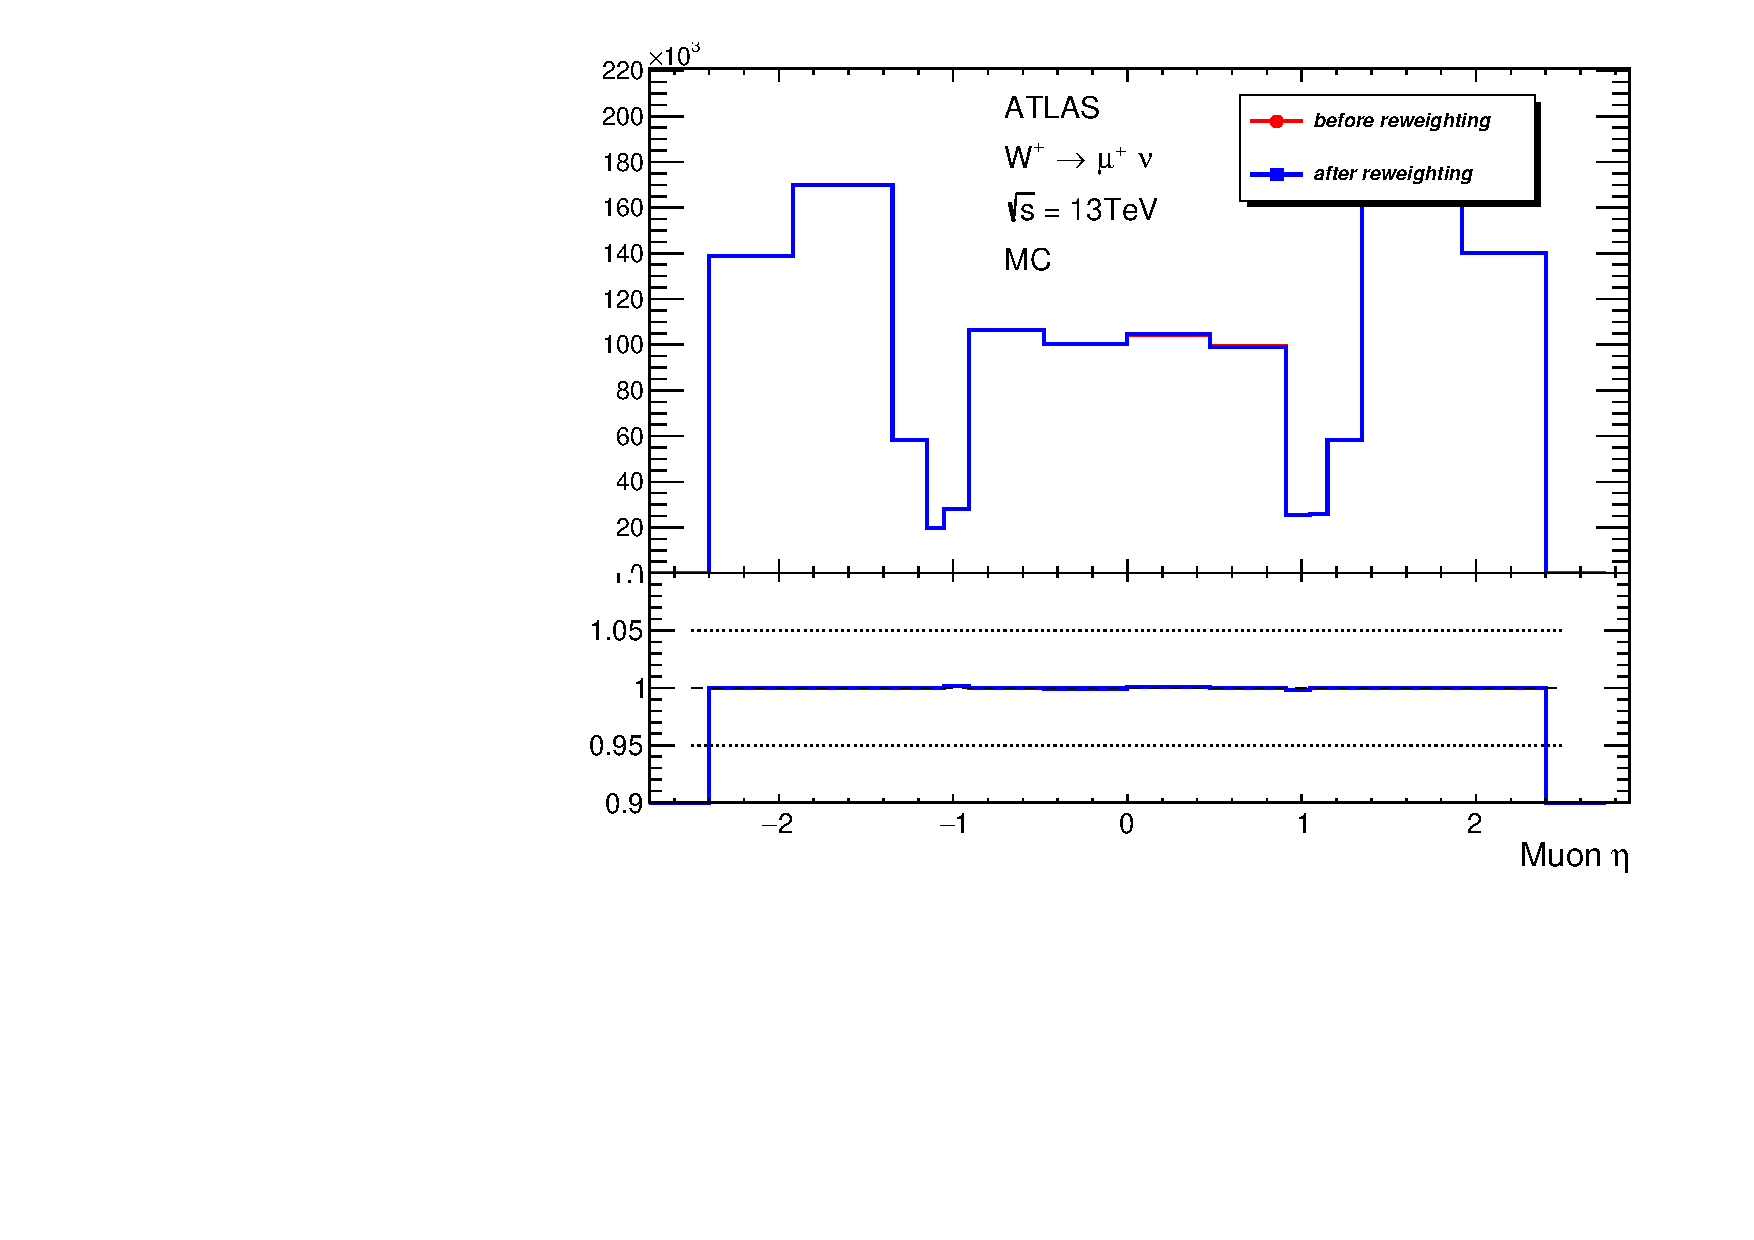
\includegraphics[width=.5\textwidth]{MC_plusmunu_WlEta_cut7_13TeV_0404_0708.pdf}%
	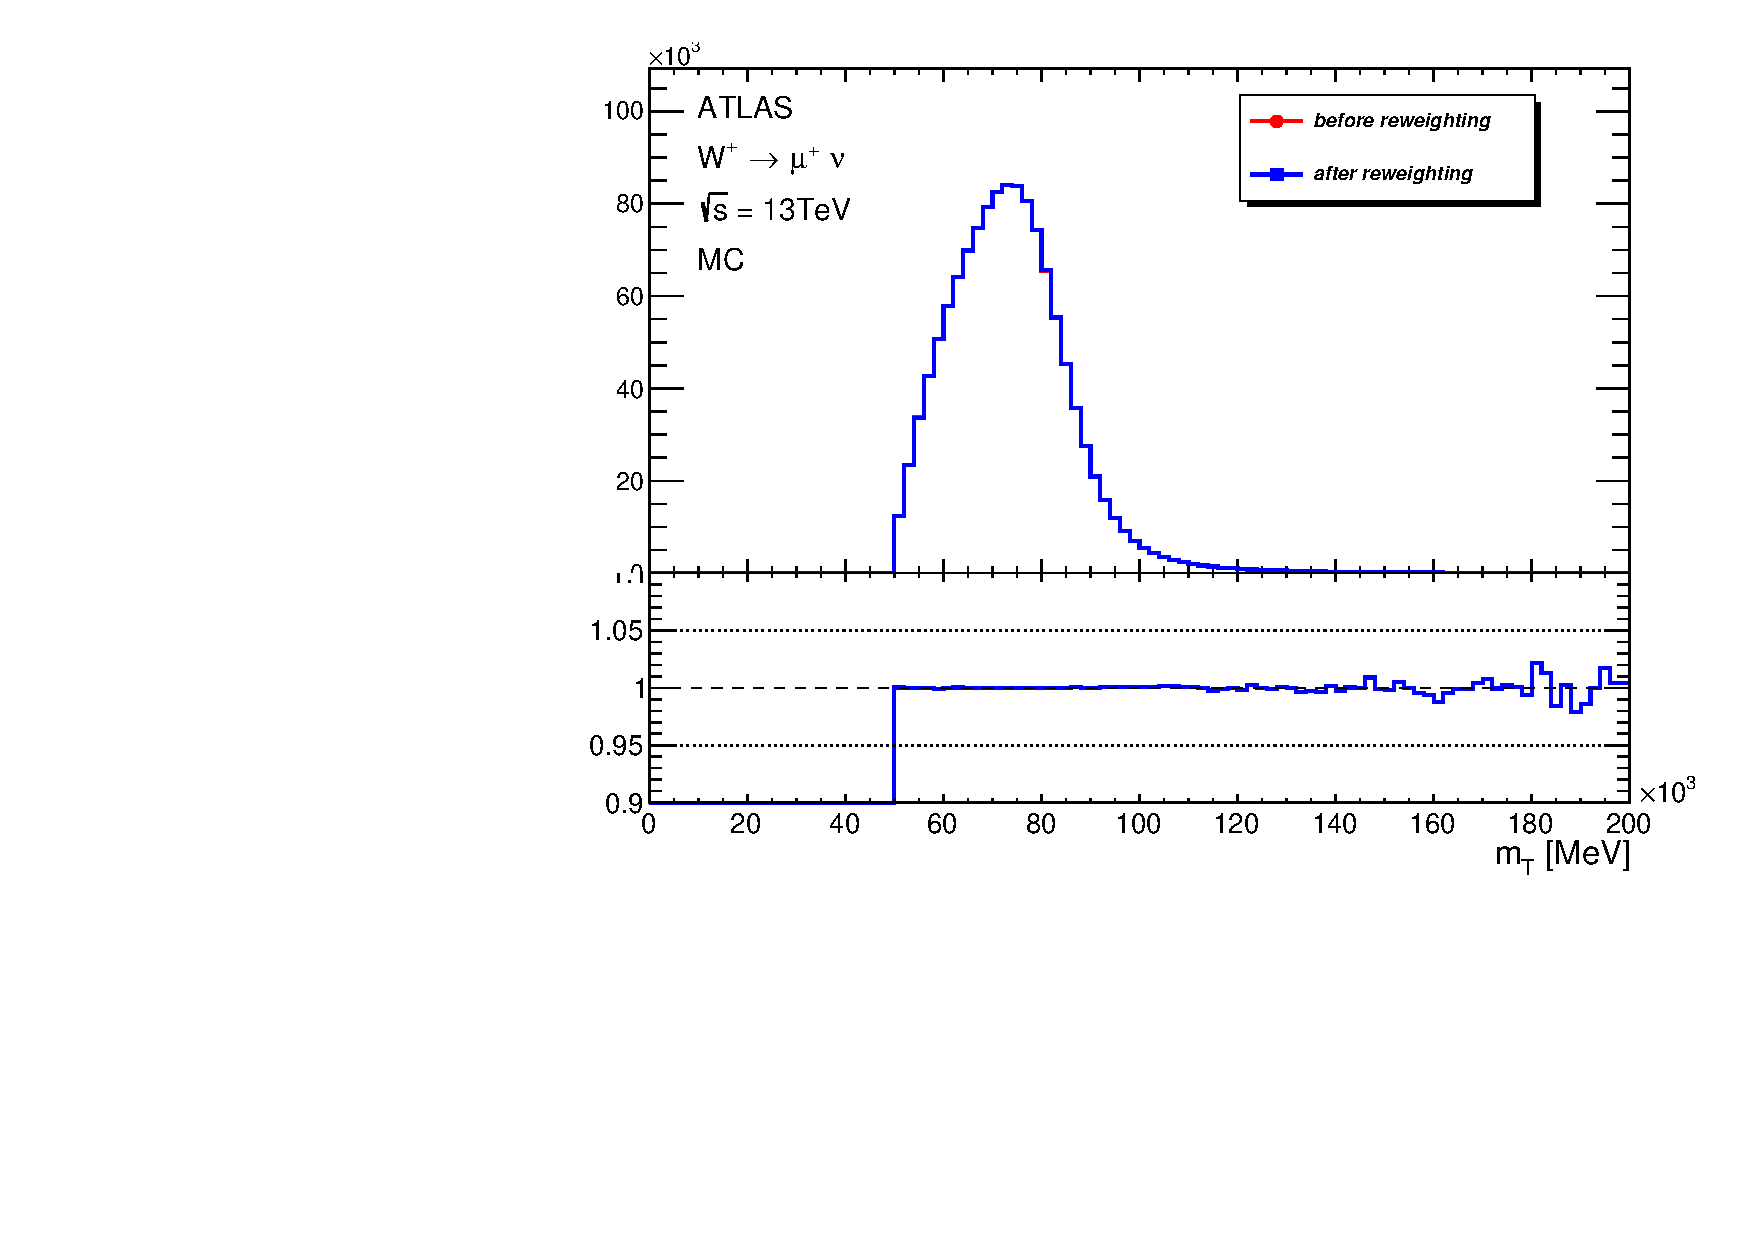
\includegraphics[width=.5\textwidth]{MC_plusmunu_WmT_cut7_13TeV_0404_0708.pdf}
	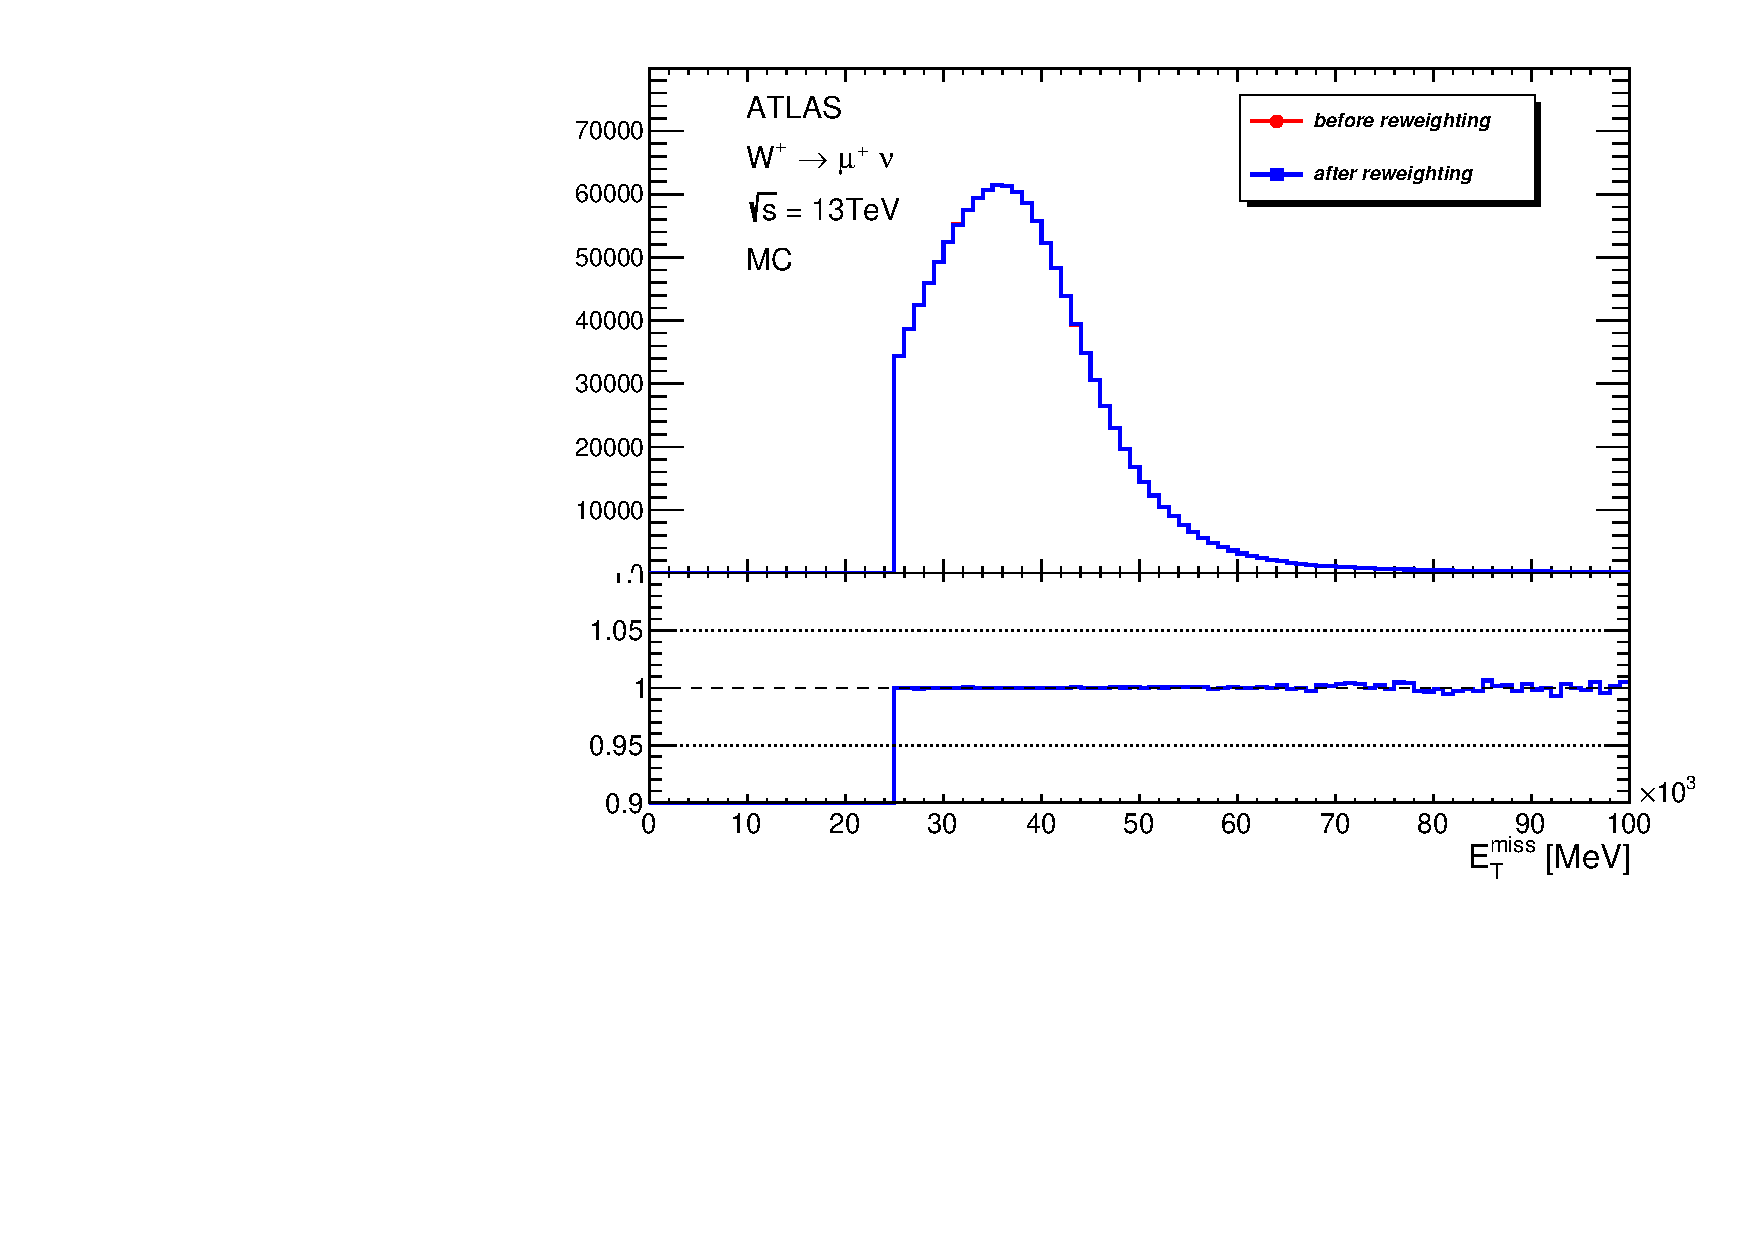
\includegraphics[width=.5\textwidth]{MC_plusmunu_Wmet_cut7_13TeV_0404_0708.pdf}%
	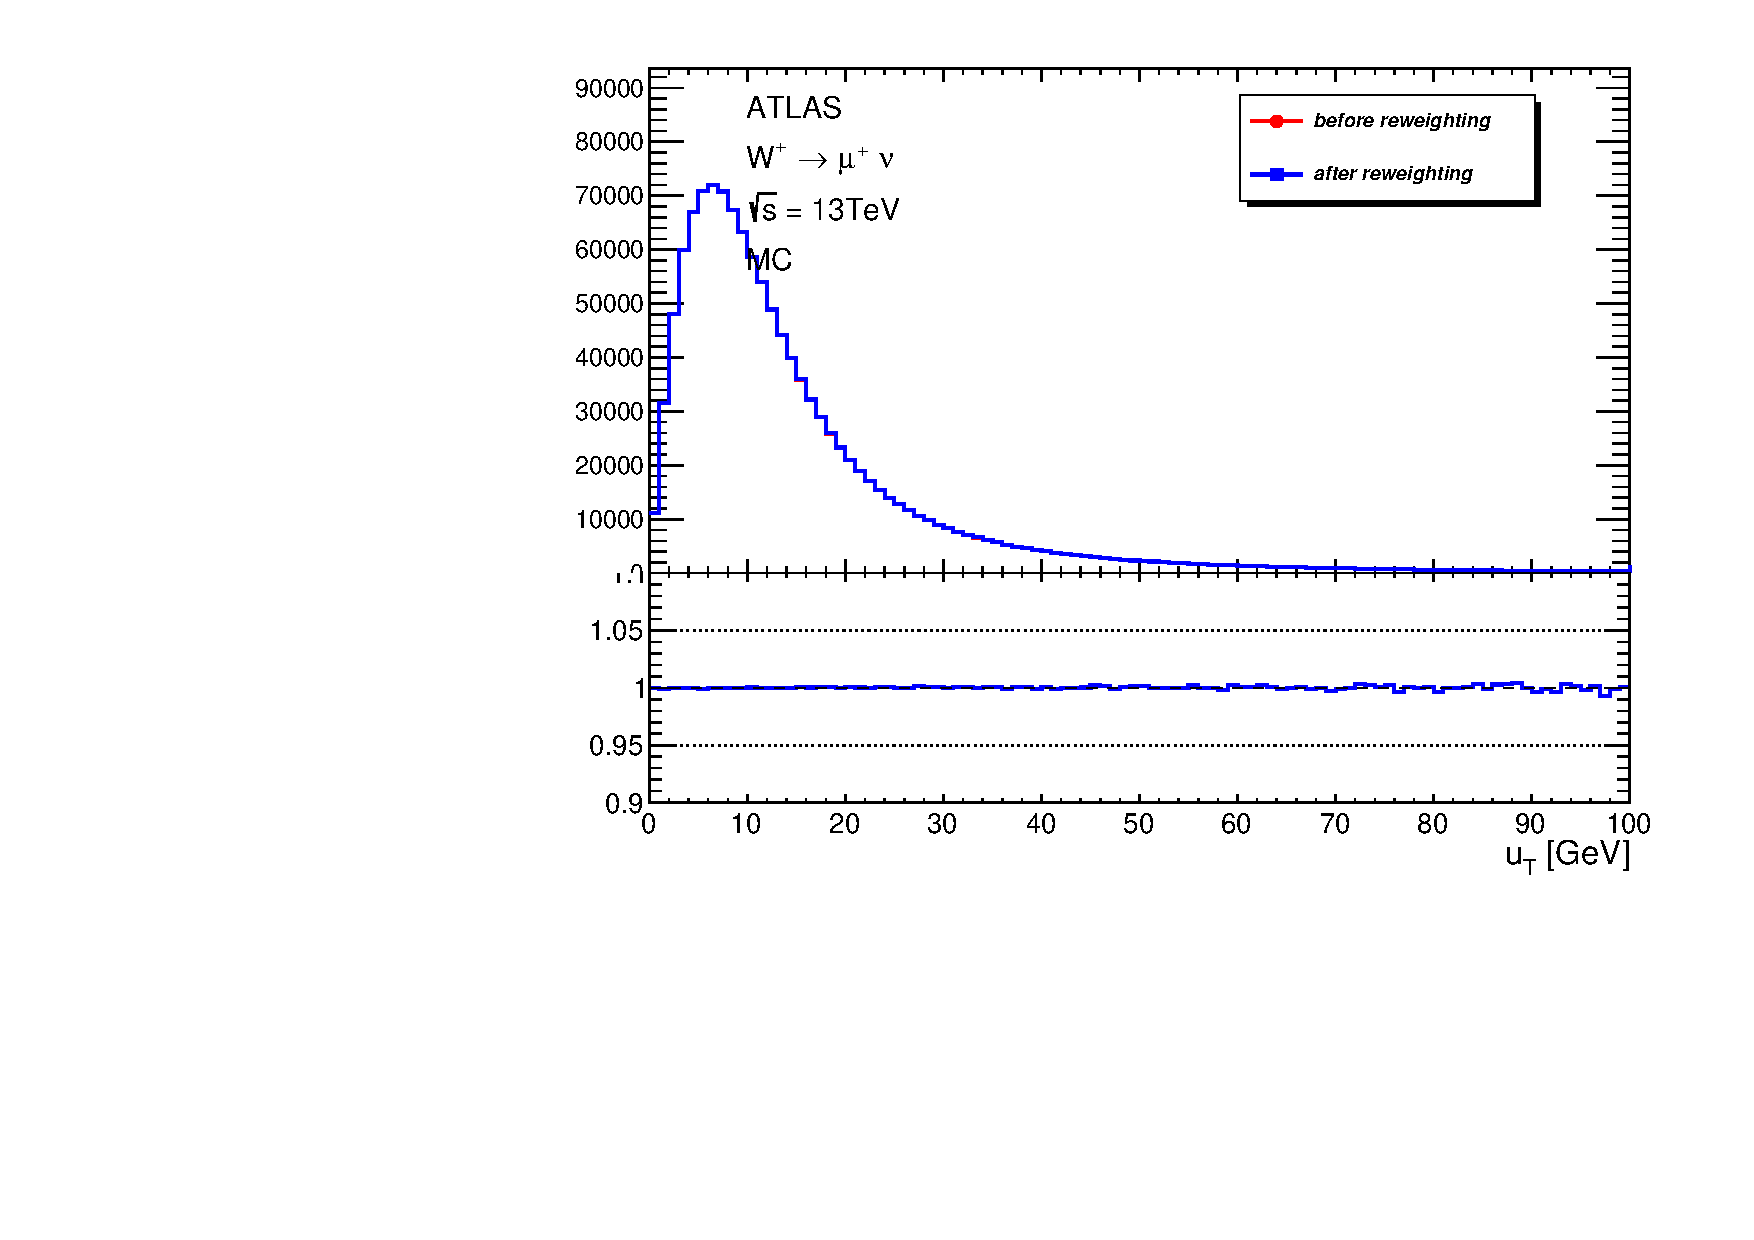
\includegraphics[width=.5\textwidth]{MC_plusmunu_WWpT_Reco_cut7_13TeV_0404_0708.pdf}
	\caption{Distributions for 13 \TeV{} 
		low-$\mu$ dataset(s) in a $W^{+}$ (top row) and a $W^{-}$ (bottom row)
		selection in electron (left) and muon (right) channels. The combined 2017 and 2018 data (black) is compared to W MC signal before (red) and after (blue) the reweighting.
		All distributions are normalised to the same number of
		selected events in 2017+2018 dataset~\cite{int_note_samples}.}
	\label{fig:observables_wzvtx}
\end{figure}

The procedure of the vertex reweighting follows the ideology of the W mass measurement performed at 7 TeV~\cite{wboson}. Despite the effect of the reweighting was found to be small for the measurement of the W boson transverse spectrum, the reweighting might still have a notable effect on the W mass measurement, that would use the obtained W pT spectrum as an input. 
A possible way to estimate the effect of the reweighting on the W boson mass is to use a template fit. The method of the template fits is described in more detail in the internal note for the 7 TeV measurement~\cite{Wmass7TeVIntNote}. Considering the observables that are sensitive to $m_W$ we can estimate the shift of the W mass value due to the reweighting. The results for $W\rightarrow \mu \nu$ channel are provided in the Table \ref{tab::z_vert_template}. They demonstrate a non-negligible effect.
\begin{table}
\centering
\begin{tabular}{|c| c| c| c|}
	\hline
	Observable & $m_T$ & $E_T^{miss}$  & $p_T^{\l}$ \\
	\hline
	$\Delta m_W$& 1.4 MeV&  5.1 MeV & 0.2 MeV \\
	\hline
\end{tabular}\\
\caption{Estimate of the Z vertex reweighting effect on the W boson mass.}
\label{tab::z_vert_template}
\end{table}


\section{W analysis event selection and control plots}
\label{sec:selection}

\subsection{Event selection}
\label{subsec:wselection}
In both cases of 5 and 13~\TeV\, events with \Wln{} candidate were selected based on a single-lepton trigger requirement.
The trigger for \Wen event candidate $\texttt{HLT\_e15\_lhloose\_nod0\_L1EM12}$, requires at least one reconstructed electron with \ET larger than 15~\GeV\ passing \emph{loose} identification requirements. Candidates for \Wmn were triggered by $\texttt{HLT\_mu14}$ trigger, requiring one medium muon with \ET larger than 14~\GeV.

Events are required to contain exactly one lepton (muon or electron) candidate having $p_T > 25\gev$. Electrons are required to have $|\eta|<2.47$ excluding transition region $1.37 < |\eta|< 1.52$. Muons   
Events with additional leptons of the same flavour with transverse momentum greater than 20 ~\GeV{} satisfying some ID criteria are discarded, to better reject the \Zboson\ background. The ID point is $medium$ for the muon channel, and $loose$ for the electron channel. There is no requirement on the number of leptons from the different channel than the channel under study.

To suppress background, in particular from multijet processes,
events are required to have \MET{} greater than 25~\GeV{}.
The \Wboson{} boson transverse mass \mt{} is demanded to be larger than 50~\GeV.
This transverse mass is defined as follows:

\begin{equation}\label{eq:mt}
{m}_{T} = \sqrt{2 {p}_{T}^{\nu}p_{T} ^{l} (1-\cos\Delta\phi^{\nu})}
\end{equation}

Tables~\ref{tab:wpen5},\ref{tab:wpmn5},\ref{tab:wmen5},\ref{tab:wmmn5} contain signal selection event yields for the $W^{\pm} \rightarrow \ell^{\pm}\nu$  at $\sqrt{s} = 5~\TeV$ \lowmu dataset. Similarly the tables~\ref{tab:wpen},\ref{tab:wpmn},\ref{tab:wmen},\ref{tab:wmmn} contain the corresponding numbers for the 13~\TeV\ \lowmu\ dataset. The listed uncertainties are statistical. Table~\ref{tab:wyields} provides a comparison between observed and expected yields.
Events denoted as \Wln{} in the tables and the plots contain the sum of background events coming from \Wtaunu\ and \Wboson{} leptonic decays other than the signal.


\begin{table}[h] 
\resizebox{\textwidth}{!}{% 
\begin{tabular}{c|ccc|ccc|ccc|ccc|ccc|ccc|ccc} \toprule
\multicolumn{1}{c}{Cut} &  \multicolumn{3}{c}{Data}  &  \multicolumn{3}{c}{Signal}  &  \multicolumn{3}{c}{$W^{\pm} \rightarrow \ell^{\pm}\nu$ BG}  &  \multicolumn{3}{c}{$Z \rightarrow \ell\ell$}  &  \multicolumn{3}{c}{Top}  &  \multicolumn{3}{c}{Diboson}  &  \multicolumn{3}{c}{Multijet}  \\  \midrule 
One electron & & 1993720 &  & 643610 & $ \pm $ & 260 & 32940 & $ \pm $ & 190 & 44338 & $ \pm $ & 71 & 1754.4 & $ \pm $ & 3.9 & 772.2 & $ \pm $ & 3.7 & & - &  \\
Electron trig matched & & 1907724 &  & 612940 & $ \pm $ & 250 & 30790 & $ \pm $ & 190 & 42100 & $ \pm $ & 69 & 1698.5 & $ \pm $ & 3.8 & 741.1 & $ \pm $ & 3.6 & & - &  \\
Isolation & & 1438941 &  & 610320 & $ \pm $ & 250 & 30590 & $ \pm $ & 190 & 41923 & $ \pm $ & 69 & 1663.6 & $ \pm $ & 3.8 & 722.5 & $ \pm $ & 3.6 & & - &  \\
$p_{T}^{e}>25 \mathrm{GeV}$ & & 720284 &  & 482240 & $ \pm $ & 220 & 14790 & $ \pm $ & 130 & 31955 & $ \pm $ & 53 & 1464.5 & $ \pm $ & 3.5 & 592.1 & $ \pm $ & 3.2 & & - &  \\
$E_{T}^{miss}>25 \mathrm{GeV}$ & & 440605 &  & 421510 & $ \pm $ & 210 & 9650 & $ \pm $ & 100 & 1336 & $ \pm $ & 20 & 1223 & $ \pm $ & 3.2 & 420.8 & $ \pm $ & 2.4 & & - &  \\
$m_{T}>50 \mathrm{GeV}$ & & 430620 &  & 417430 & $ \pm $ & 210 & 8800 & $ \pm $ & 96 & 1047 & $ \pm $ & 16 & 944.3 & $ \pm $ & 2.9 & 373.5 & $ \pm $ & 2.2 & 3030 & $ \pm $ & 550 \\
\bottomrule
\end{tabular}}
\caption{Analysis cut flow for $W^+ \rightarrow e^+\nu$ 5 TeV signal selection. Lepton \pt\ is required to be over 18~\GeV{} before the final cut.}
\label{tab:wpen5}
\end{table}

\begin{table}[h] 
\resizebox{\textwidth}{!}{% 
\begin{tabular}{c|ccc|ccc|ccc|ccc|ccc|ccc|ccc} \toprule
\multicolumn{1}{c}{Cut} &  \multicolumn{3}{c}{Data}  &  \multicolumn{3}{c}{Signal}  &  \multicolumn{3}{c}{$W^{\pm} \rightarrow \ell^{\pm}\nu$ BG}  &  \multicolumn{3}{c}{$Z \rightarrow \ell\ell$}  &  \multicolumn{3}{c}{Top}  &  \multicolumn{3}{c}{Diboson}  &  \multicolumn{3}{c}{Multijet}  \\  \midrule 
One electron & & 7915023 &  & 1797340 & $ \pm $ & 390 & 92520 & $ \pm $ & 270 & 147490 & $ \pm $ & 140 & 63207 & $ \pm $ & 89 & 3069 & $ \pm $ & 63 & & - &  \\
Electron trig matched & & 7840239 &  & 1709140 & $ \pm $ & 380 & 86370 & $ \pm $ & 260 & 139760 & $ \pm $ & 140 & 61110 & $ \pm $ & 88 & 2967 & $ \pm $ & 62 & & - &  \\
Isolation & & 5413483 &  & 1698430 & $ \pm $ & 380 & 85560 & $ \pm $ & 260 & 138890 & $ \pm $ & 140 & 59834 & $ \pm $ & 87 & 2939 & $ \pm $ & 61 & & - &  \\
$p_{T}^{e}>25 \mathrm{GeV}$ & & 2452868 &  & 1342200 & $ \pm $ & 330 & 44450 & $ \pm $ & 190 & 106270 & $ \pm $ & 110 & 53811 & $ \pm $ & 82 & 2565 & $ \pm $ & 58 & & - &  \\
$E_{T}^{miss}>25 \mathrm{GeV}$ & & 1275513 &  & 1136520 & $ \pm $ & 310 & 28580 & $ \pm $ & 150 & 8313 & $ \pm $ & 46 & 45707 & $ \pm $ & 75 & 1990 & $ \pm $ & 53 & & - &  \\
$m_{T}>50 \mathrm{GeV}$ & & 1207776 &  & 1117560 & $ \pm $ & 310 & 24760 & $ \pm $ & 130 & 6443 & $ \pm $ & 36 & 34580 & $ \pm $ & 65 & 1718 & $ \pm $ & 50 & 28000 & $ \pm $ & 1800 \\
\bottomrule
\end{tabular}}
\caption{Analysis cut flow for $W^+ \rightarrow e^+\nu$ 13 TeV signal selection. Lepton \pt\ is required to be over 18~\GeV{} before the final cut.}
\label{tab:wpen}
\end{table}

\begin{table}[h] 
\resizebox{\textwidth}{!}{% 
\begin{tabular}{c|ccc|ccc|ccc|ccc|ccc|ccc|ccc} \toprule
\multicolumn{1}{c}{Cut} &  \multicolumn{3}{c}{Data}  &  \multicolumn{3}{c}{Signal}  &  \multicolumn{3}{c}{$W^{\pm} \rightarrow \ell^{\pm}\nu$ BG}  &  \multicolumn{3}{c}{$Z \rightarrow \ell\ell$}  &  \multicolumn{3}{c}{Top}  &  \multicolumn{3}{c}{Diboson}  &  \multicolumn{3}{c}{Multijet}  \\  \midrule 
One muon & & 2434459 &  & 760980 & $ \pm $ & 280 & 35090 & $ \pm $ & 200 & 37015 & $ \pm $ & 82 & 2025.3 & $ \pm $ & 4.1 & 864.7 & $ \pm $ & 3.7 & & - &  \\
Muon trig matched & & 2353403 &  & 664100 & $ \pm $ & 260 & 30610 & $ \pm $ & 190 & 32554 & $ \pm $ & 76 & 1725.6 & $ \pm $ & 3.8 & 746.6 & $ \pm $ & 3.4 & & - &  \\
Isolation & & 1186616 &  & 659200 & $ \pm $ & 260 & 30400 & $ \pm $ & 190 & 32303 & $ \pm $ & 76 & 1574.6 & $ \pm $ & 3.7 & 710.1 & $ \pm $ & 3.3 & & - &  \\
$p_{T}^{\mu}>25 \mathrm{GeV}$ & & 632016 &  & 508270 & $ \pm $ & 230 & 13900 & $ \pm $ & 130 & 22556 & $ \pm $ & 57 & 1335.3 & $ \pm $ & 3.4 & 568.2 & $ \pm $ & 2.9 & & - &  \\
$E_{T}^{miss}>25 \mathrm{GeV}$ & & 470856 &  & 442600 & $ \pm $ & 210 & 8700 & $ \pm $ & 100 & 9959 & $ \pm $ & 31 & 1111.8 & $ \pm $ & 3 & 424.5 & $ \pm $ & 2.5 & & - &  \\
$m_{T}>50 \mathrm{GeV}$ & & 457053 &  & 438280 & $ \pm $ & 210 & 7879 & $ \pm $ & 97 & 9649 & $ \pm $ & 27 & 879.7 & $ \pm $ & 2.8 & 381.7 & $ \pm $ & 2.3 & 720 & $ \pm $ & 190 \\
\bottomrule
\end{tabular}}
\caption{Analysis cut flow for $W^+ \rightarrow \mu^+\nu$ 5 TeV signal selection. Lepton \pt\ is required to be over 18~\GeV{} before the final cut.}
\label{tab:wpmn5}
\end{table}

\begin{table}[h] 
\resizebox{\textwidth}{!}{% 
\begin{tabular}{c|ccc|ccc|ccc|ccc|ccc|ccc|ccc} \toprule
\multicolumn{1}{c}{Cut} &  \multicolumn{3}{c}{Data}  &  \multicolumn{3}{c}{Signal}  &  \multicolumn{3}{c}{$W^{\pm} \rightarrow \ell^{\pm}\nu$ BG}  &  \multicolumn{3}{c}{$Z \rightarrow \ell\ell$}  &  \multicolumn{3}{c}{Top}  &  \multicolumn{3}{c}{Diboson}  &  \multicolumn{3}{c}{Multijet}  \\  \midrule 
One muon & & 9570104 &  & 2100770 & $ \pm $ & 410 & 83110 & $ \pm $ & 270 & 2019400 & $ \pm $ & 2200 & 71602 & $ \pm $ & 94 & 3442 & $ \pm $ & 63 & & - &  \\
Muon trig matched & & 9382783 &  & 1840550 & $ \pm $ & 390 & 72820 & $ \pm $ & 250 & 1750400 & $ \pm $ & 2000 & 61519 & $ \pm $ & 87 & 2956 & $ \pm $ & 59 & & - &  \\
Isolation & & 3905612 &  & 1821750 & $ \pm $ & 380 & 71780 & $ \pm $ & 250 & 595700 & $ \pm $ & 1100 & 56849 & $ \pm $ & 84 & 2916 & $ \pm $ & 59 & & - &  \\
$p_{T}^{\mu}>25 \mathrm{GeV}$ & & 1930655 &  & 1393330 & $ \pm $ & 340 & 34470 & $ \pm $ & 170 & 170840 & $ \pm $ & 490 & 49338 & $ \pm $ & 78 & 2471 & $ \pm $ & 54 & & - &  \\
$E_{T}^{miss}>25 \mathrm{GeV}$ & & 1321407 &  & 1173860 & $ \pm $ & 310 & 21450 & $ \pm $ & 140 & 51090 & $ \pm $ & 180 & 41956 & $ \pm $ & 72 & 1930 & $ \pm $ & 49 & & - &  \\
$m_{T}>50 \mathrm{GeV}$ & & 1244892 &  & 1153800 & $ \pm $ & 310 & 18270 & $ \pm $ & 130 & 38304 & $ \pm $ & 81 & 32375 & $ \pm $ & 63 & 1705 & $ \pm $ & 44 & 9040 & $ \pm $ & 800 \\
\bottomrule
\end{tabular}}
\caption{Analysis cut flow for $W^+ \rightarrow \mu^+\nu$ 13 TeV signal selection. Lepton \pt\ is required to be over 18~\GeV{} before the final cut.}
\label{tab:wpmn}
\end{table}

\begin{table}[h] 
\resizebox{\textwidth}{!}{% 
\begin{tabular}{c|ccc|ccc|ccc|ccc|ccc|ccc|ccc} \toprule
\multicolumn{1}{c}{Cut} &  \multicolumn{3}{c}{Data}  &  \multicolumn{3}{c}{Signal}  &  \multicolumn{3}{c}{$W^{\pm} \rightarrow \ell^{\pm}\nu$ BG}  &  \multicolumn{3}{c}{$Z \rightarrow \ell\ell$}  &  \multicolumn{3}{c}{Top}  &  \multicolumn{3}{c}{Diboson}  &  \multicolumn{3}{c}{Multijet}  \\  \midrule 
One electron & & 1724472 &  & 374900 & $ \pm $ & 200 & 24150 & $ \pm $ & 160 & 41995 & $ \pm $ & 70 & 1590.5 & $ \pm $ & 2.9 & 684.8 & $ \pm $ & 4 & & - &  \\
Electron trig matched & & 1645694 &  & 359010 & $ \pm $ & 200 & 22070 & $ \pm $ & 160 & 39854 & $ \pm $ & 68 & 1539.9 & $ \pm $ & 2.9 & 655.7 & $ \pm $ & 3.9 & & - &  \\
Isolation & & 1176976 &  & 357660 & $ \pm $ & 200 & 21920 & $ \pm $ & 160 & 39686 & $ \pm $ & 68 & 1504.6 & $ \pm $ & 2.8 & 640.7 & $ \pm $ & 3.8 & & - &  \\
$p_{T}^{e}>25 \mathrm{GeV}$ & & 529183 &  & 302070 & $ \pm $ & 180 & 11920 & $ \pm $ & 110 & 30214 & $ \pm $ & 52 & 1330.8 & $ \pm $ & 2.6 & 532.9 & $ \pm $ & 3.5 & & - &  \\
$E_{T}^{miss}>25 \mathrm{GeV}$ & & 281957 &  & 266750 & $ \pm $ & 170 & 8084 & $ \pm $ & 90 & 1293 & $ \pm $ & 20 & 1112.5 & $ \pm $ & 2.4 & 380 & $ \pm $ & 3 & & - &  \\
$m_{T}>50 \mathrm{GeV}$ & & 274329 &  & 264540 & $ \pm $ & 170 & 7317 & $ \pm $ & 84 & 994 & $ \pm $ & 16 & 855.2 & $ \pm $ & 2.1 & 338.1 & $ \pm $ & 2.9 & 2400 & $ \pm $ & 500 \\
\bottomrule
\end{tabular}}
\caption{Analysis cut flow for $W^- \rightarrow e^-\nu$ 5 TeV signal selection. Lepton \pt\ is required to be over 18~\GeV{} before the final cut.}
\label{tab:wmen5}
\end{table}

\begin{table}[h] 
\resizebox{\textwidth}{!}{% 
\begin{tabular}{c|ccc|ccc|ccc|ccc|ccc|ccc|ccc} \toprule
\multicolumn{1}{c}{Cut} &  \multicolumn{3}{c}{Data}  &  \multicolumn{3}{c}{Signal}  &  \multicolumn{3}{c}{$W^{\pm} \rightarrow \ell^{\pm}\nu$ BG}  &  \multicolumn{3}{c}{$Z \rightarrow \ell\ell$}  &  \multicolumn{3}{c}{Top}  &  \multicolumn{3}{c}{Diboson}  &  \multicolumn{3}{c}{Multijet}  \\  \midrule 
One electron & & 7471742 &  & 1323710 & $ \pm $ & 330 & 78230 & $ \pm $ & 230 & 140980 & $ \pm $ & 140 & 61951 & $ \pm $ & 86 & 3059 & $ \pm $ & 58 & & - &  \\
Electron trig matched & & 7402574 &  & 1267710 & $ \pm $ & 330 & 72240 & $ \pm $ & 230 & 133580 & $ \pm $ & 140 & 59950 & $ \pm $ & 85 & 2968 & $ \pm $ & 57 & & - &  \\
Isolation & & 4949352 &  & 1260540 & $ \pm $ & 330 & 71550 & $ \pm $ & 230 & 132740 & $ \pm $ & 140 & 58689 & $ \pm $ & 84 & 2937 & $ \pm $ & 57 & & - &  \\
$p_{T}^{e}>25 \mathrm{GeV}$ & & 2113364 &  & 1053510 & $ \pm $ & 300 & 39660 & $ \pm $ & 160 & 101350 & $ \pm $ & 110 & 52923 & $ \pm $ & 79 & 2544 & $ \pm $ & 53 & & - &  \\
$E_{T}^{miss}>25 \mathrm{GeV}$ & & 1008915 &  & 900640 & $ \pm $ & 280 & 25900 & $ \pm $ & 130 & 7954 & $ \pm $ & 45 & 45065 & $ \pm $ & 73 & 1962 & $ \pm $ & 48 & & - &  \\
$m_{T}>50 \mathrm{GeV}$ & & 949362 &  & 887810 & $ \pm $ & 270 & 22400 & $ \pm $ & 120 & 6052 & $ \pm $ & 35 & 34177 & $ \pm $ & 64 & 1695 & $ \pm $ & 44 & 27400 & $ \pm $ & 2000 \\
\bottomrule
\end{tabular}}
\caption{Analysis cut flow for $W^- \rightarrow e^-\nu$ 13 TeV signal selection. Lepton \pt\ is required to be over 18~\GeV{} before the final cut.}
\label{tab:wmen}
\end{table}

\begin{table}[h] 
\resizebox{\textwidth}{!}{% 
\begin{tabular}{c|ccc|ccc|ccc|ccc|ccc|ccc|ccc} \toprule
\multicolumn{1}{c}{Cut} &  \multicolumn{3}{c}{Data}  &  \multicolumn{3}{c}{Signal}  &  \multicolumn{3}{c}{$W^{\pm} \rightarrow \ell^{\pm}\nu$ BG}  &  \multicolumn{3}{c}{$Z \rightarrow \ell\ell$}  &  \multicolumn{3}{c}{Top}  &  \multicolumn{3}{c}{Diboson}  &  \multicolumn{3}{c}{Multijet}  \\  \midrule 
One muon & & 2075709 &  & 440560 & $ \pm $ & 220 & 22510 & $ \pm $ & 170 & 34440 & $ \pm $ & 80 & 1835.6 & $ \pm $ & 3.1 & 751.5 & $ \pm $ & 3.3 & & - &  \\
Muon trig matched & & 2002955 &  & 383720 & $ \pm $ & 200 & 19640 & $ \pm $ & 160 & 30277 & $ \pm $ & 75 & 1561.6 & $ \pm $ & 2.9 & 648 & $ \pm $ & 3.1 & & - &  \\
Isolation & & 883078 &  & 381010 & $ \pm $ & 200 & 19450 & $ \pm $ & 160 & 30046 & $ \pm $ & 74 & 1411 & $ \pm $ & 2.7 & 616.9 & $ \pm $ & 2.9 & & - &  \\
$p_{T}^{\mu}>25 \mathrm{GeV}$ & & 426119 &  & 314370 & $ \pm $ & 180 & 9370 & $ \pm $ & 110 & 20749 & $ \pm $ & 56 & 1202.1 & $ \pm $ & 2.5 & 505 & $ \pm $ & 2.5 & & - &  \\
$E_{T}^{miss}>25 \mathrm{GeV}$ & & 298992 &  & 276060 & $ \pm $ & 170 & 5893 & $ \pm $ & 89 & 8716 & $ \pm $ & 29 & 1004.2 & $ \pm $ & 2.3 & 372.6 & $ \pm $ & 2 & & - &  \\
$m_{T}>50 \mathrm{GeV}$ & & 287870 &  & 273710 & $ \pm $ & 170 & 5158 & $ \pm $ & 82 & 8408 & $ \pm $ & 26 & 788.2 & $ \pm $ & 2 & 335.6 & $ \pm $ & 1.9 & 760 & $ \pm $ & 160 \\
\bottomrule
\end{tabular}}
\caption{Analysis cut flow for $W^- \rightarrow \mu^-\nu$ 5 TeV signal selection. Lepton \pt\ is required to be over 18~\GeV{} before the final cut.}
\label{tab:wmmn5}
\end{table}

\begin{table}[h] 
\resizebox{\textwidth}{!}{% 
\begin{tabular}{c|ccc|ccc|ccc|ccc|ccc|ccc|ccc} \toprule
\multicolumn{1}{c}{Cut} &  \multicolumn{3}{c}{Data}  &  \multicolumn{3}{c}{Signal}  &  \multicolumn{3}{c}{$W^{\pm} \rightarrow \ell^{\pm}\nu$ BG}  &  \multicolumn{3}{c}{$Z \rightarrow \ell\ell$}  &  \multicolumn{3}{c}{Top}  &  \multicolumn{3}{c}{Diboson}  &  \multicolumn{3}{c}{Multijet}  \\  \midrule 
One muon & & 8773414 &  & 1518070 & $ \pm $ & 360 & 64930 & $ \pm $ & 230 & 2019900 & $ \pm $ & 2200 & 70580 & $ \pm $ & 90 & 3230 & $ \pm $ & 60 & & - &  \\
Muon trig matched & & 8597493 &  & 1322980 & $ \pm $ & 330 & 56520 & $ \pm $ & 210 & 1750300 & $ \pm $ & 2000 & 60579 & $ \pm $ & 84 & 2806 & $ \pm $ & 56 & & - &  \\
Isolation & & 3298569 &  & 1310310 & $ \pm $ & 330 & 55680 & $ \pm $ & 210 & 593700 & $ \pm $ & 1100 & 55949 & $ \pm $ & 80 & 2751 & $ \pm $ & 55 & & - &  \\
$p_{T}^{\mu}>25 \mathrm{GeV}$ & & 1561721 &  & 1069770 & $ \pm $ & 300 & 28230 & $ \pm $ & 150 & 166810 & $ \pm $ & 490 & 48544 & $ \pm $ & 75 & 2362 & $ \pm $ & 52 & & - &  \\
$E_{T}^{miss}>25 \mathrm{GeV}$ & & 1030406 &  & 910150 & $ \pm $ & 280 & 17380 & $ \pm $ & 120 & 47370 & $ \pm $ & 180 & 41259 & $ \pm $ & 69 & 1842 & $ \pm $ & 46 & & - &  \\
$m_{T}>50 \mathrm{GeV}$ & & 963568 &  & 896850 & $ \pm $ & 270 & 14710 & $ \pm $ & 110 & 34572 & $ \pm $ & 80 & 31772 & $ \pm $ & 61 & 1598 & $ \pm $ & 43 & 9050 & $ \pm $ & 620 \\
\bottomrule
\end{tabular}}
\caption{Analysis cut flow for $W^- \rightarrow \mu^-\nu$ 13 TeV signal selection. Lepton \pt\ is required to be over 18~\GeV{} before the final cut.}
\label{tab:wmmn}
\end{table}

\begin{table}[h] 
\centering
\begin{tabular}{c|ccc|ccc} \toprule
\multicolumn{1}{c}{Selection} & \multicolumn{3}{c}{Observed} & \multicolumn{3}{c}{Expected} \\ \midrule
$5\TeV  \;  W^+ \rightarrow e^+\nu$  & & 430620 & & 431620 & $ \pm $ & 600\\
$5\TeV  \;  W^+ \rightarrow \mu^+\nu$ & & 457053 & & 457790 & $ \pm $ & 300\\
$5\TeV  \;  W^- \rightarrow e^-\nu$ & & 274329 & & 276450 & $ \pm $ & 530\\
$5\TeV  \;  W^- \rightarrow \mu^-\nu$ & & 287870 & & 289160 & $ \pm $ & 250\\
$13\TeV  \;  W^+ \rightarrow e^+\nu$  & & 1207776 & & 1213000 & $ \pm $ & 1800\\
$13\TeV  \;  W^+ \rightarrow \mu^+\nu$ & & 1244892 & & 1253490 & $ \pm $ & 870\\
$13\TeV  \;  W^- \rightarrow e^-\nu$ & & 949362 & & 979500 & $ \pm $ & 2000\\
$13\TeV  \;  W^- \rightarrow \mu^-\nu$ & & 963568 & & 988560 & $ \pm $ & 690\\
\bottomrule
\end{tabular}
\caption{Observed and Expected yield comparison for all signal selections.}
\label{tab:wyields}
\end{table}


%\clearpage


\subsection{$\sqrt{s} = 13$~\TeV\ dataset control plots}
\label{subsec:controlplots13}
Control plots for the 13~\TeV\ \lowmu\ dataset are provided here after applying all corrections described in Section 7, and after applying the selection described above in this section. In each figure, the right(left)-hand column shows distributions for the \Wplus\ (\Wminus) process. The top (bottom) row shows the muon (electron) decay channel. In the ratio panels, the grey band is the total systematic uncertainty, whilst the brown band adds the MC statistical uncertainty in quadrature on top of it. In regions of the distributions insensitive to the modelling of \ptw\ there is generally good agreement between data and predictions. The bulk of the \mt\ distribution is a typical example of distribution that is mostly insensitive to the modelling of \ptw. The \ut\ distribution depends a lot on the modelling of the W boson transverse momentum and it demonstrates the highest discrepancy between the data and MC. Therefore it can be concluded that the baseline simulation is not modelling \ptw\ satisfactorily.
\newpage
%%%%%%%%%%%%%%%%%%%%%%%%%%%%%%%%_log.
%%%%% ************************* 13 TeV ****************************
%%%%%%%%%%%%%%%%%%%%%%%%%%%%%%%%


\begin{figure}[h]
	\centering
	{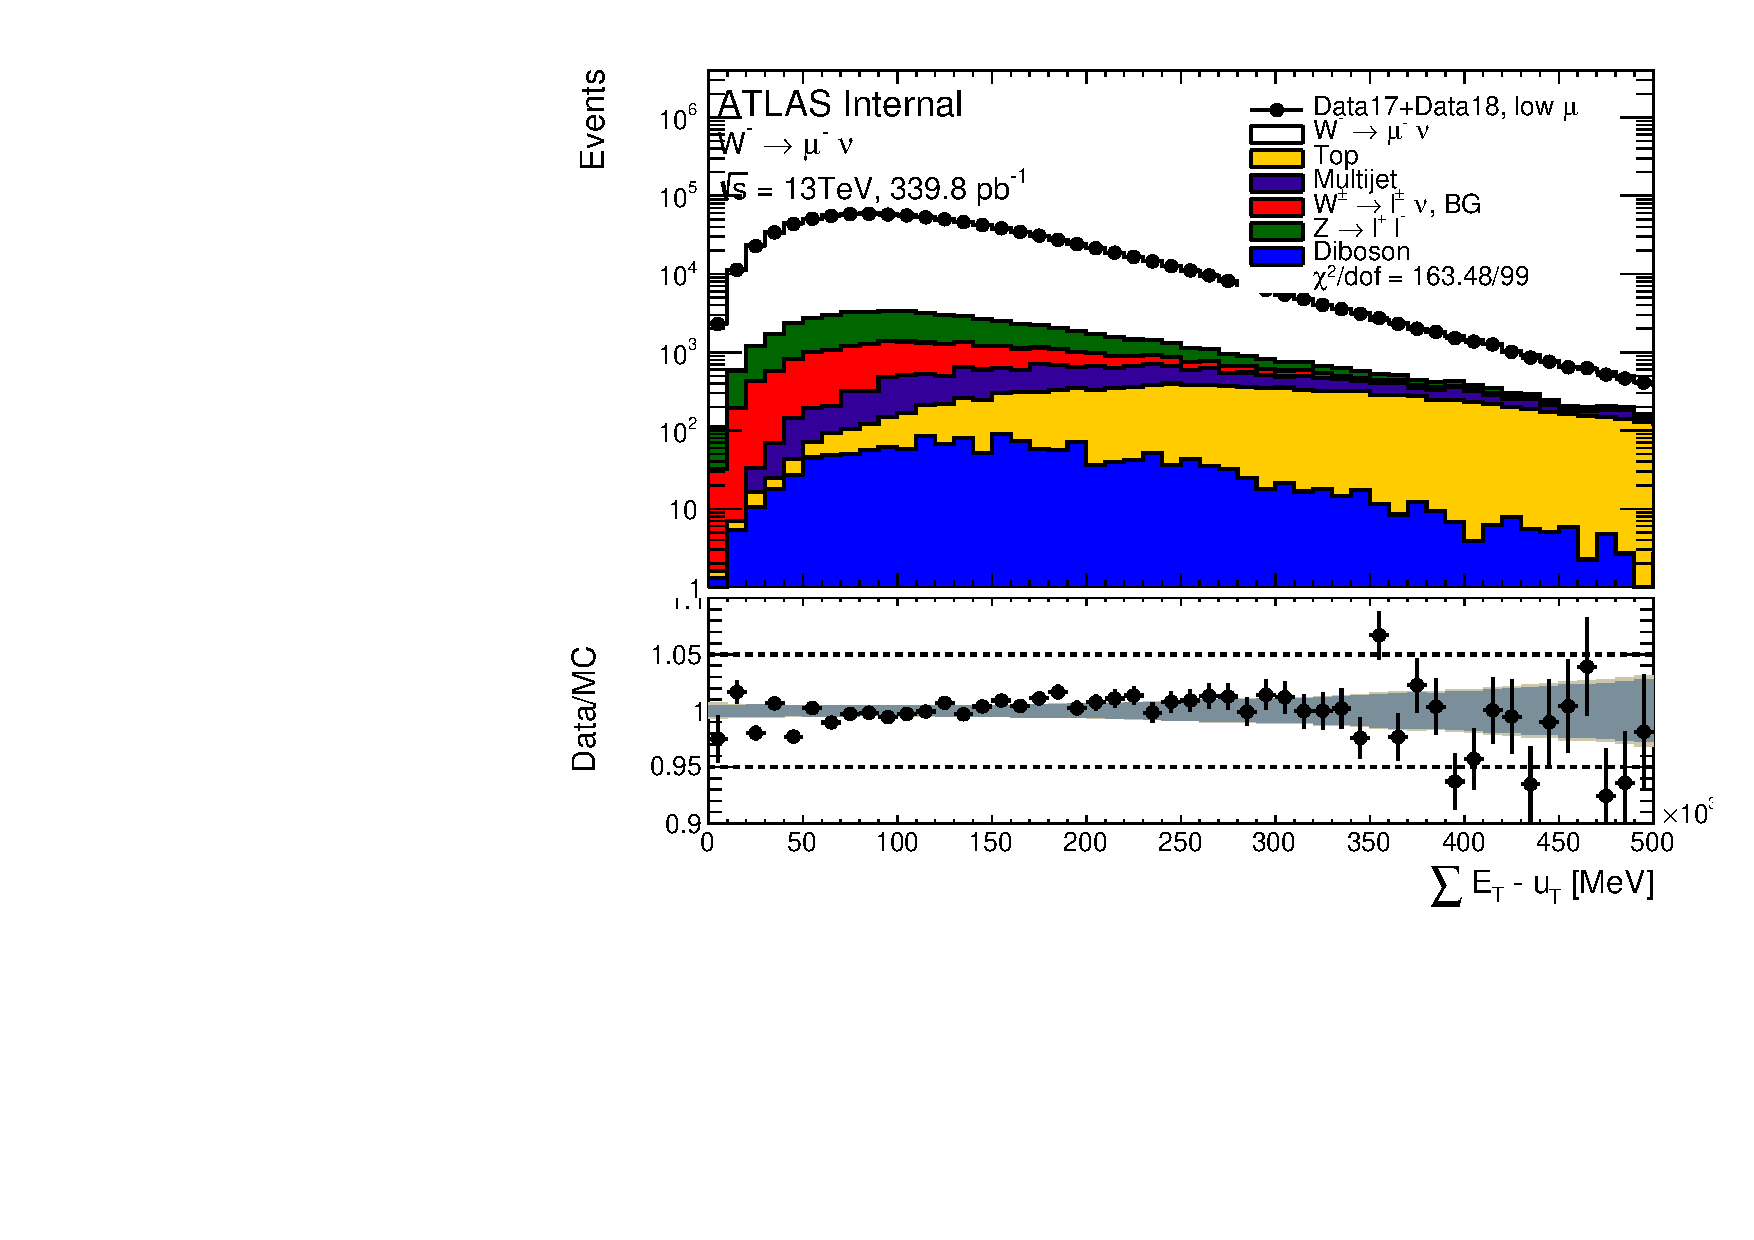
\includegraphics[width=.49\textwidth]{control_norm/SETUE_cut7_minusmunu_13TeV_log_norm_NormErr.pdf}\label{f:SETUEmm13}}
	{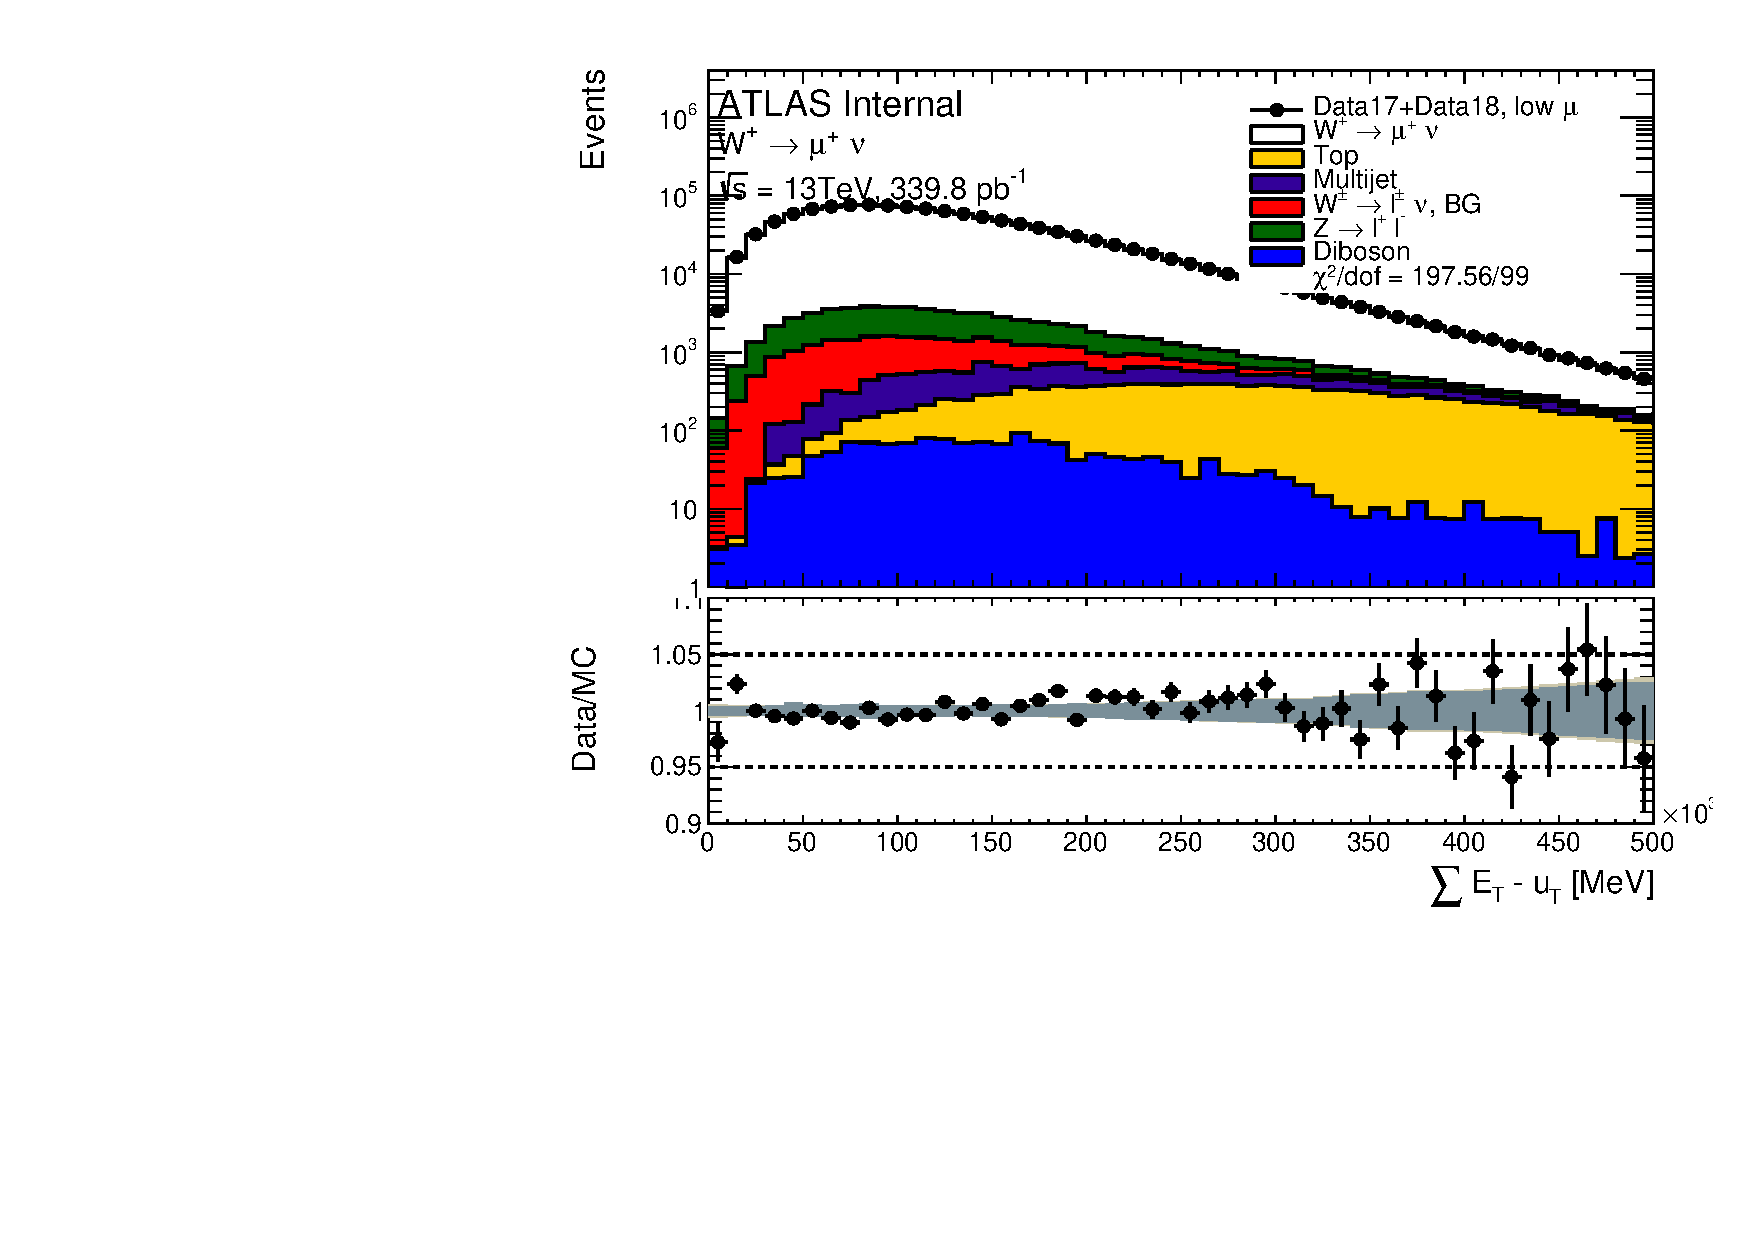
\includegraphics[width=.49\textwidth]{control_norm/SETUE_cut7_plusmunu_13TeV_log_norm_NormErr.pdf}\label{f:SETUEpm13}}
	
	{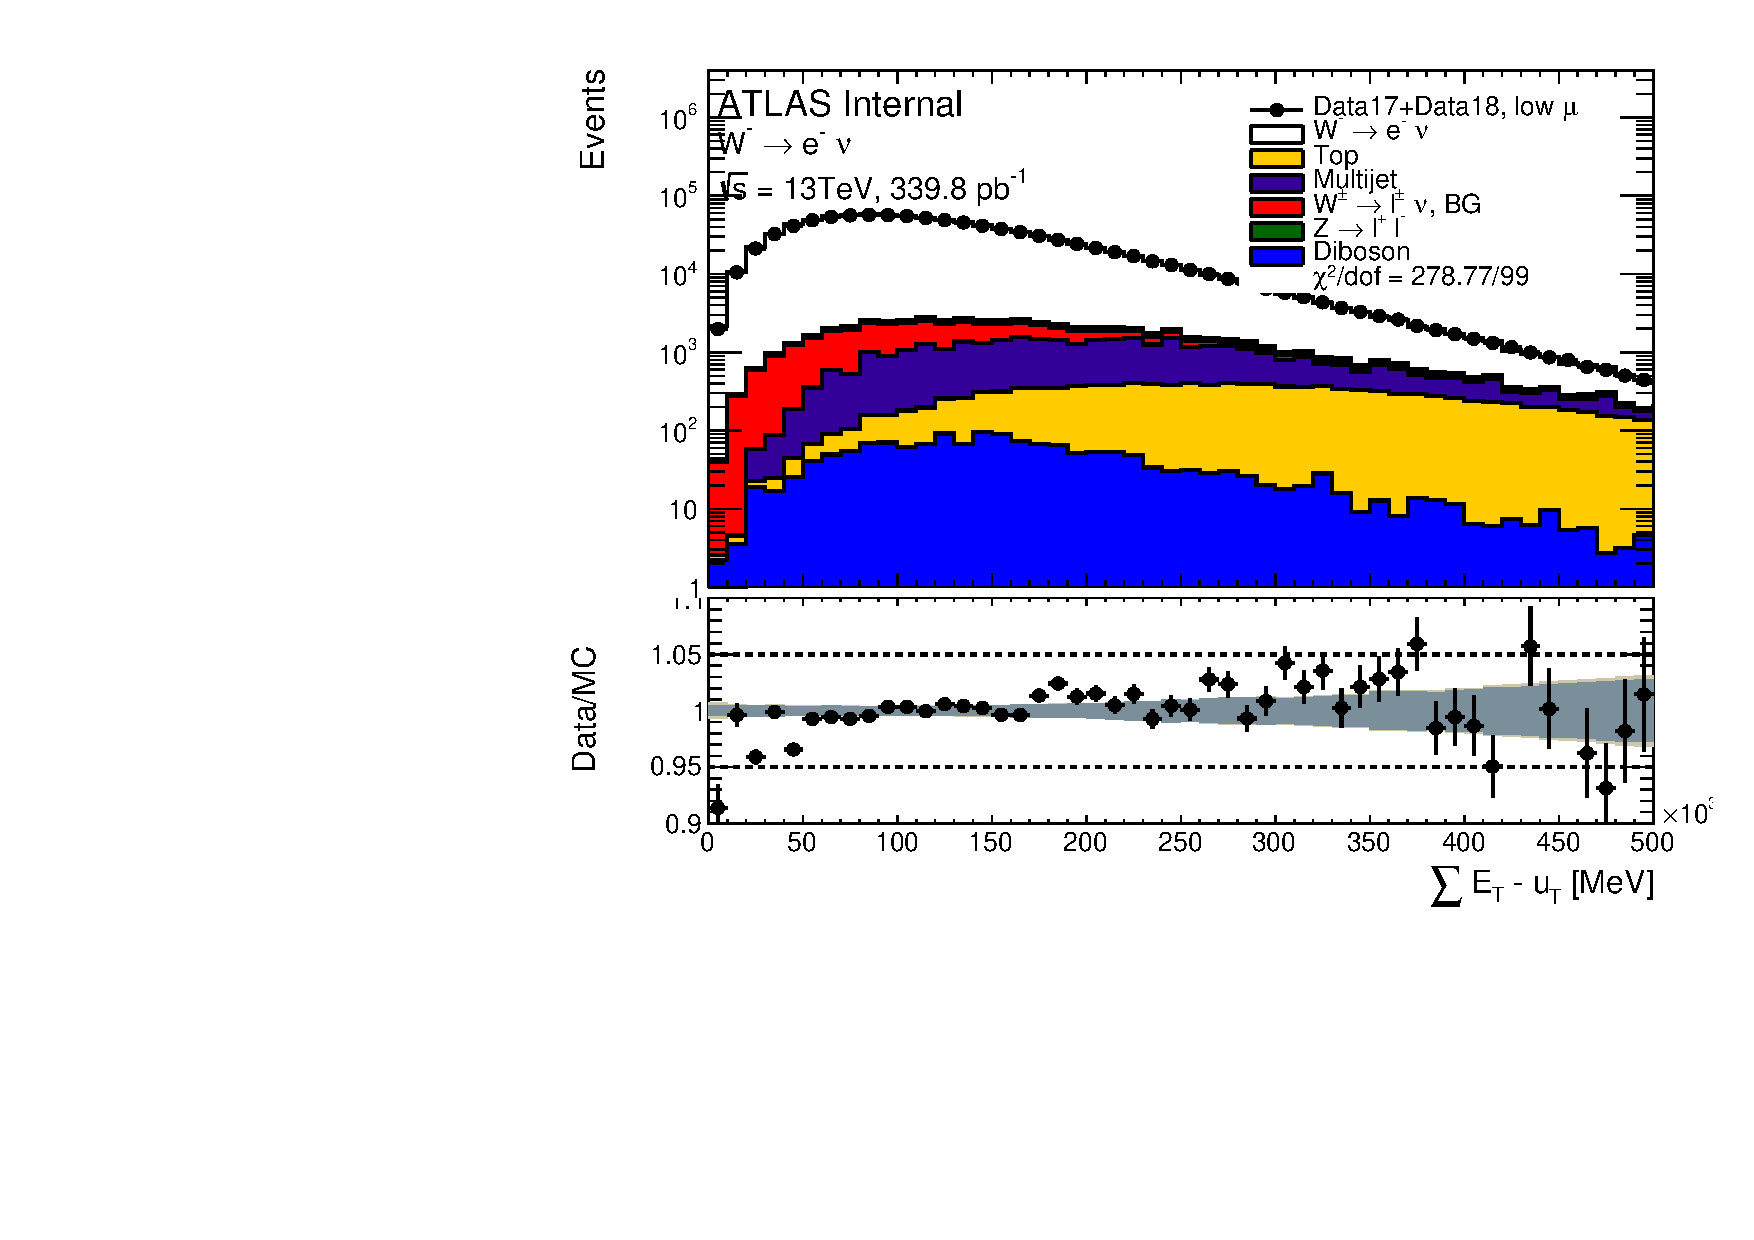
\includegraphics[width=.49\textwidth]{control_norm/SETUE_cut7_minusenu_13TeV_log_norm_NormErr.pdf}\label{f:}}
	{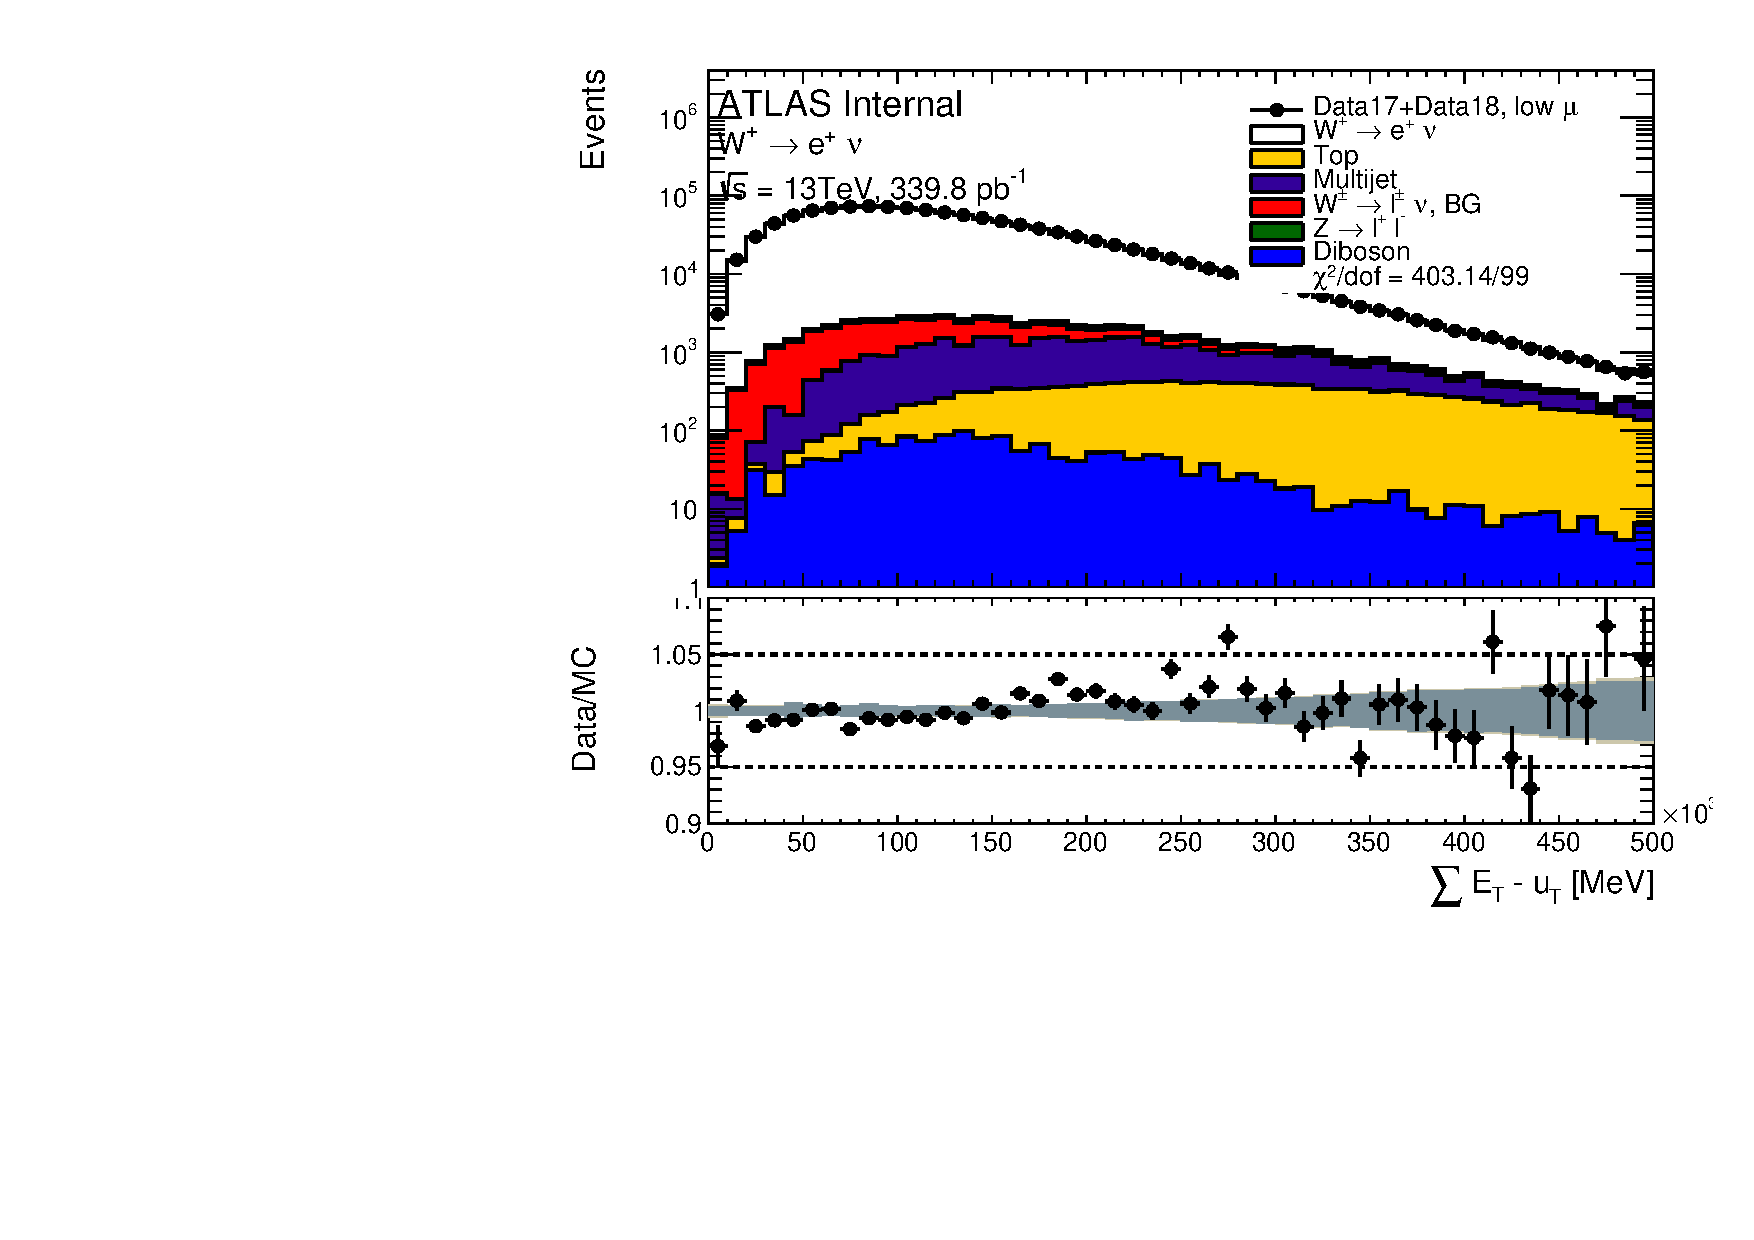
\includegraphics[width=.49\textwidth]{control_norm/SETUE_cut7_plusenu_13TeV_log_norm_NormErr.pdf}\label{f:}}
	\caption{$\Sigma \bar{E_T}$ distribution in the muon and electron channel  for the $\sqrt{s} = 13$~\TeV\ dataset.}\end{figure}
%

\begin{figure}[h]
	\centering
	{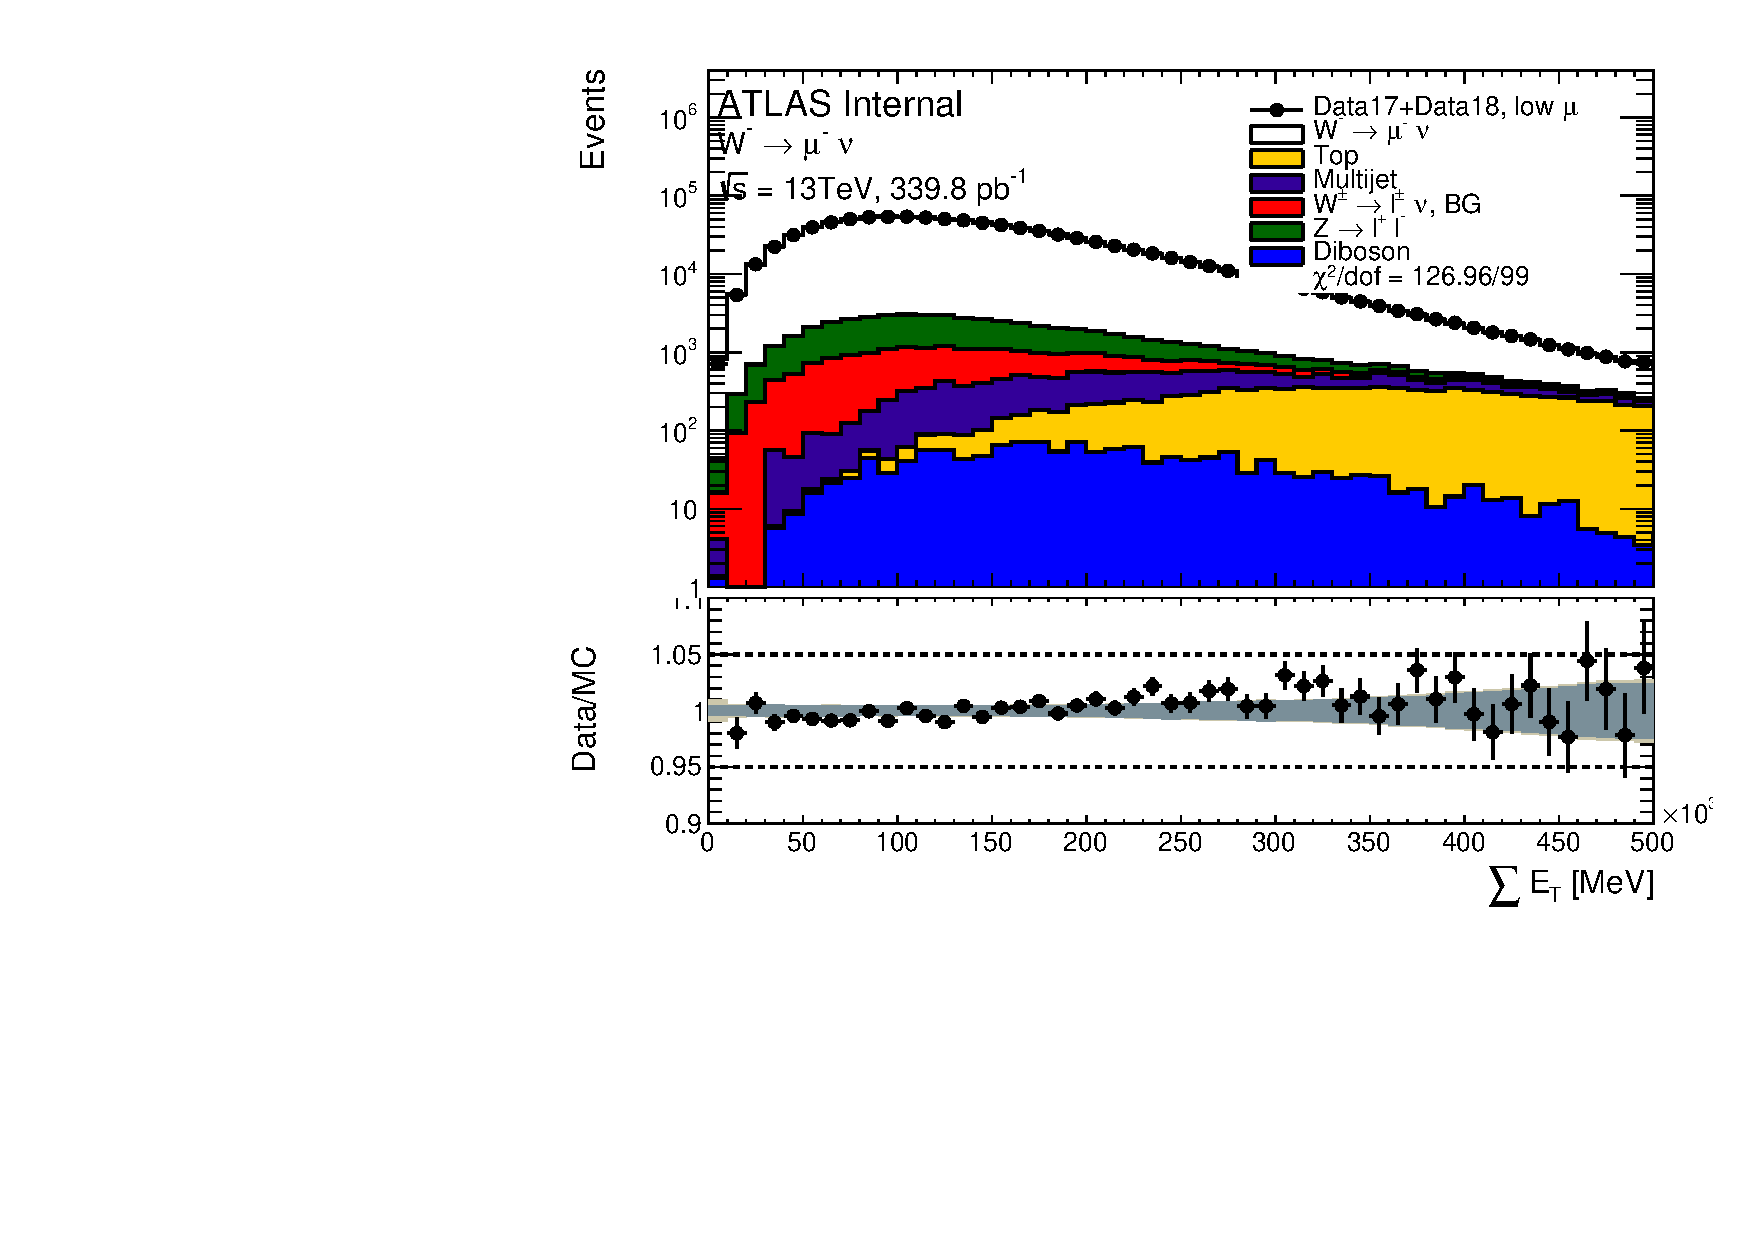
\includegraphics[width=.49\textwidth]{control_norm/SET_cut7_minusmunu_13TeV_log_norm_NormErr.pdf}\label{f:set13}}
	{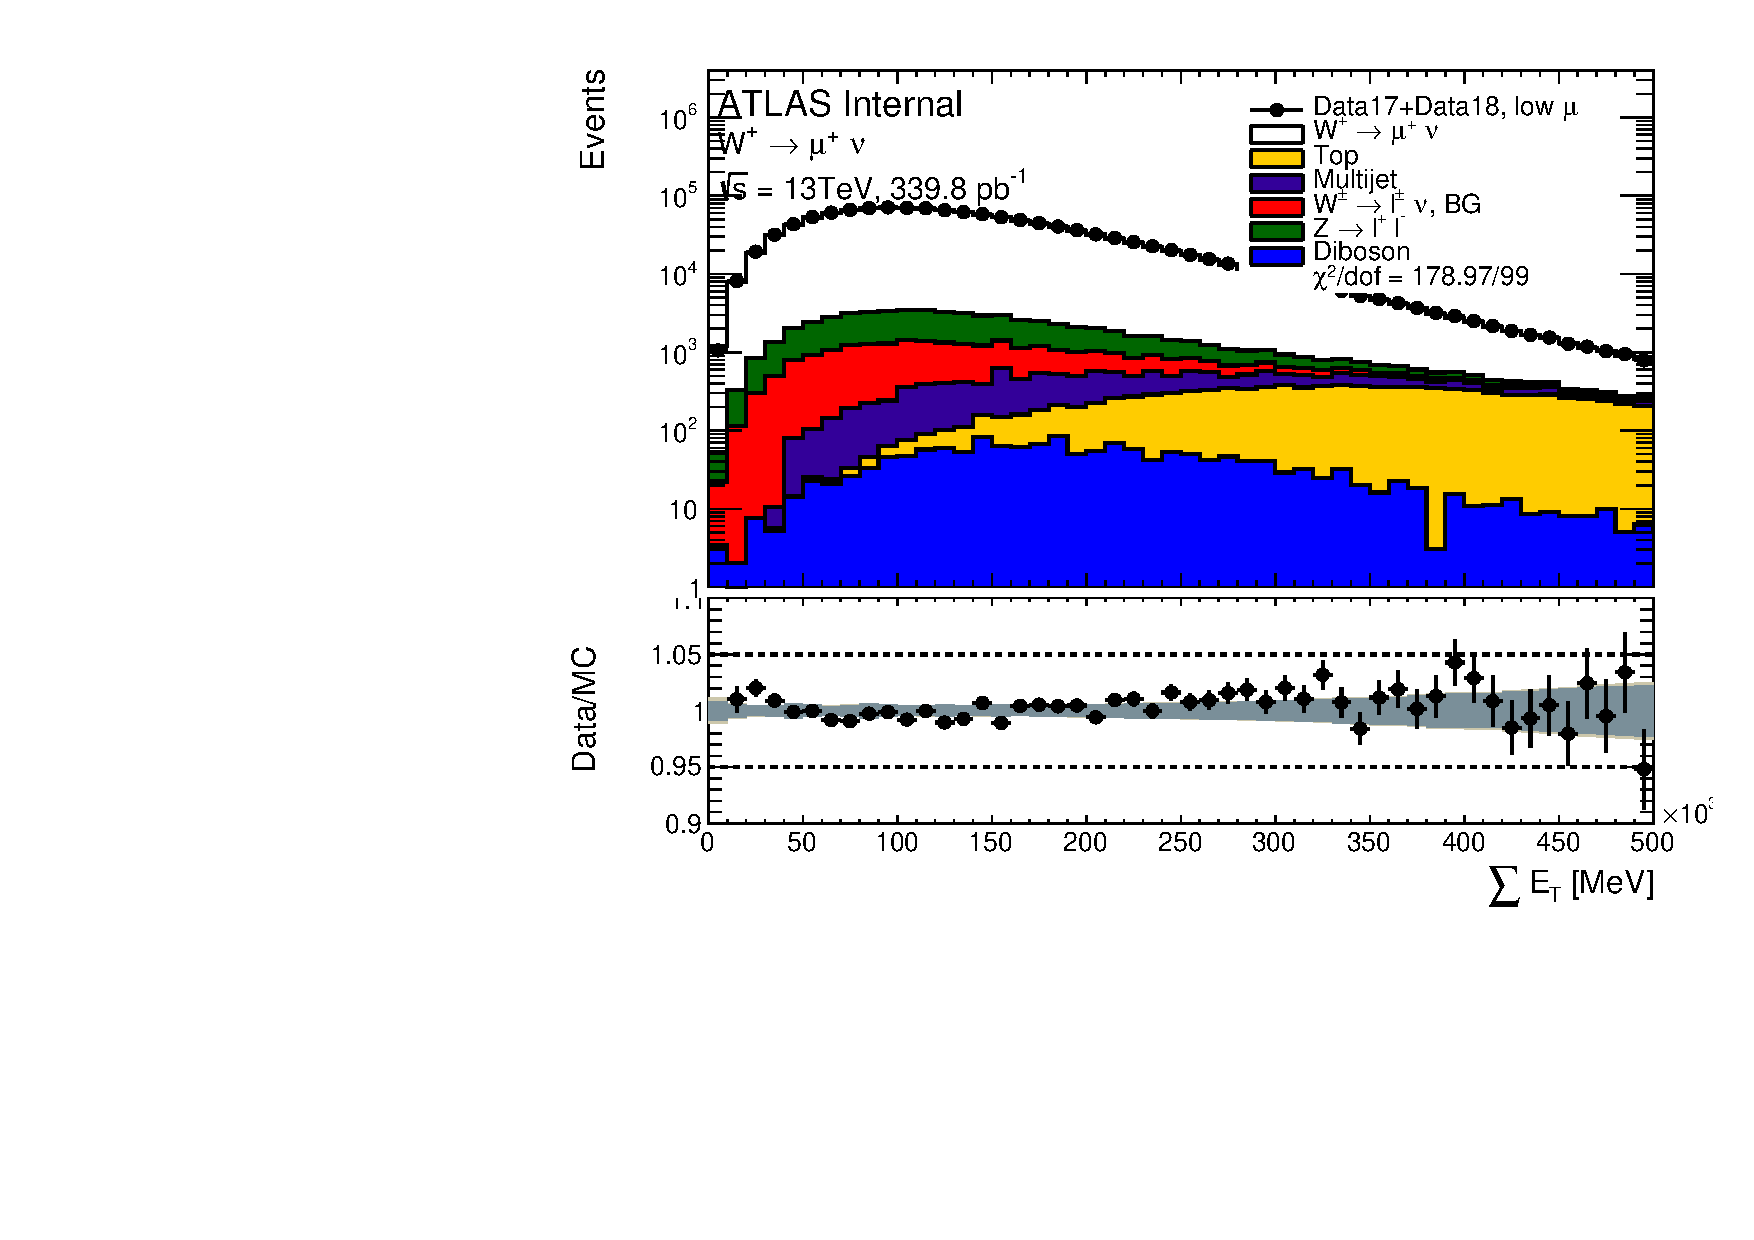
\includegraphics[width=.49\textwidth]{control_norm/SET_cut7_plusmunu_13TeV_log_norm_NormErr.pdf}\label{f:setpl}}
	
	{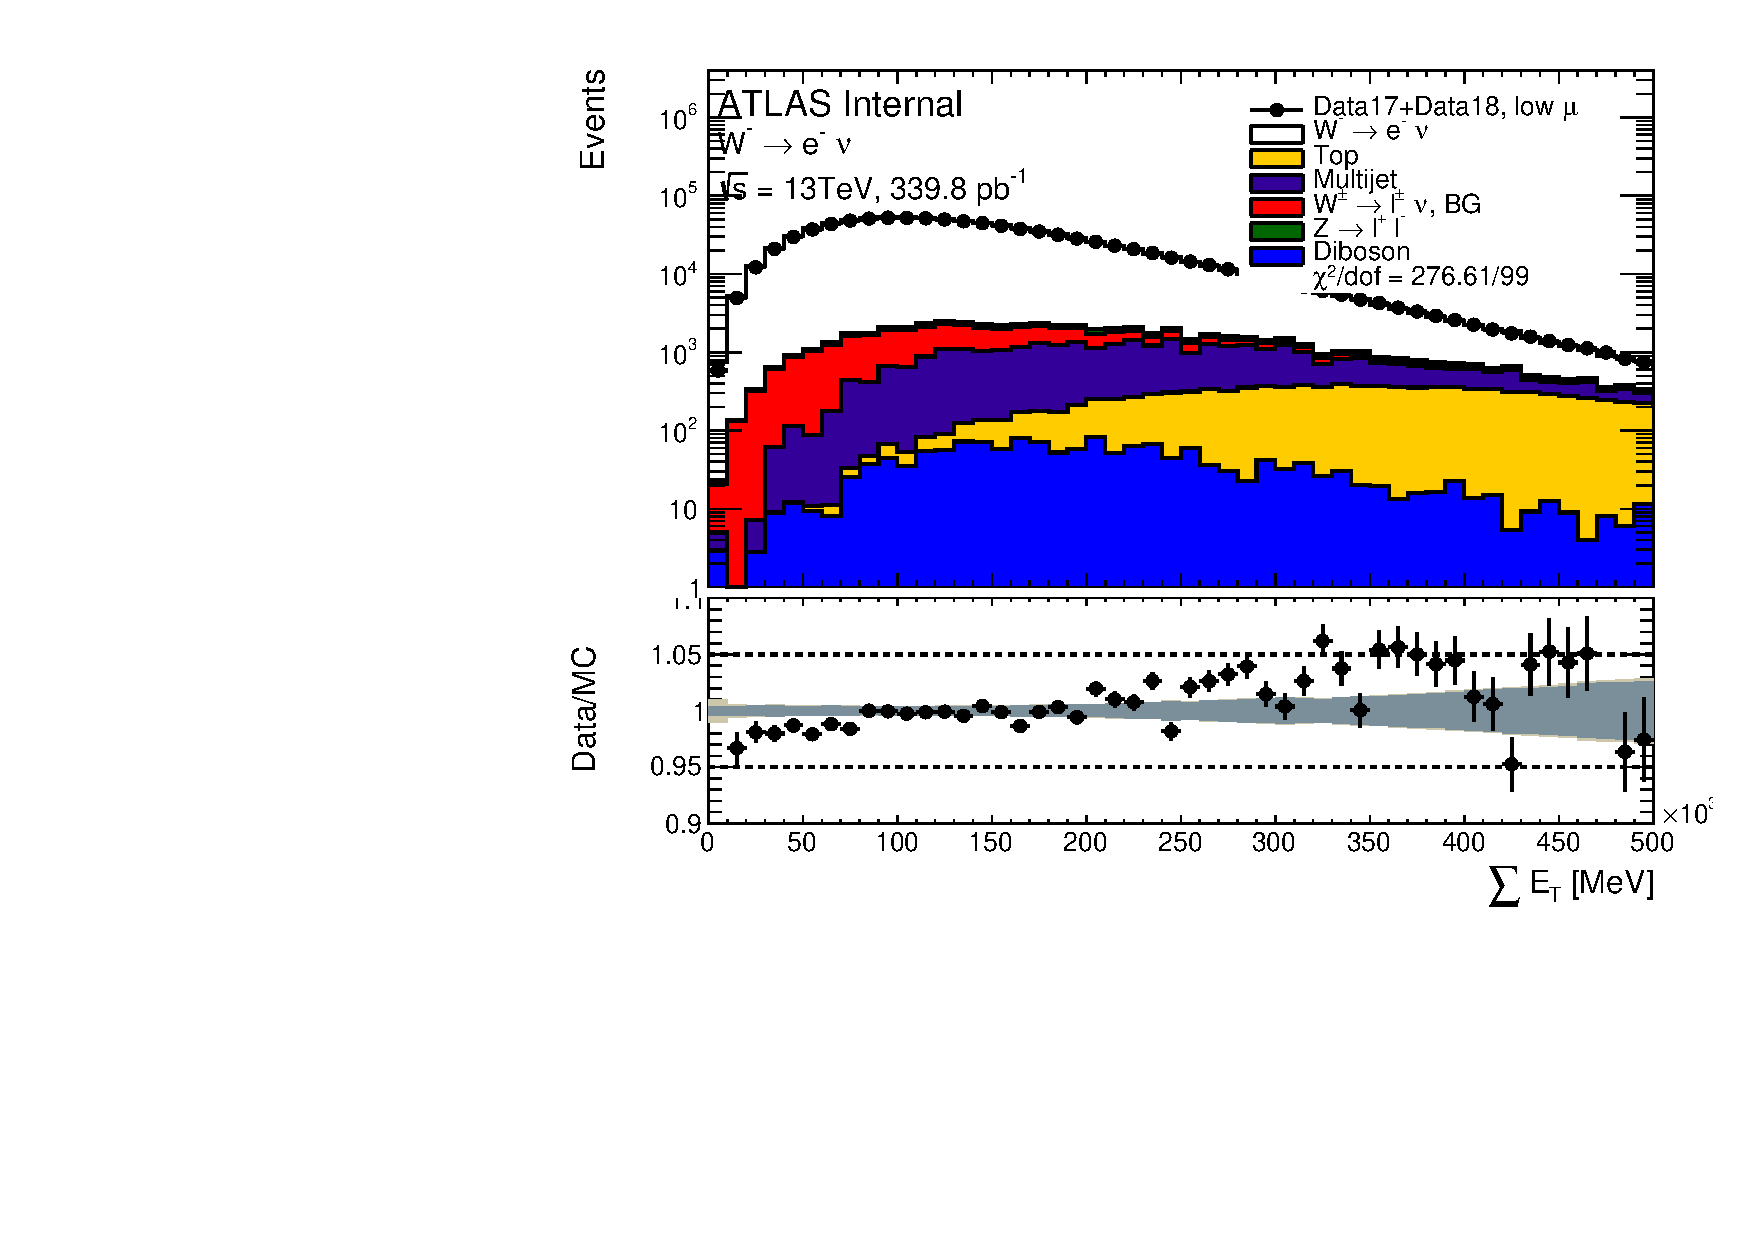
\includegraphics[width=.49\textwidth]{control_norm/SET_cut7_minusenu_13TeV_log_norm_NormErr.pdf}\label{f:}}
	{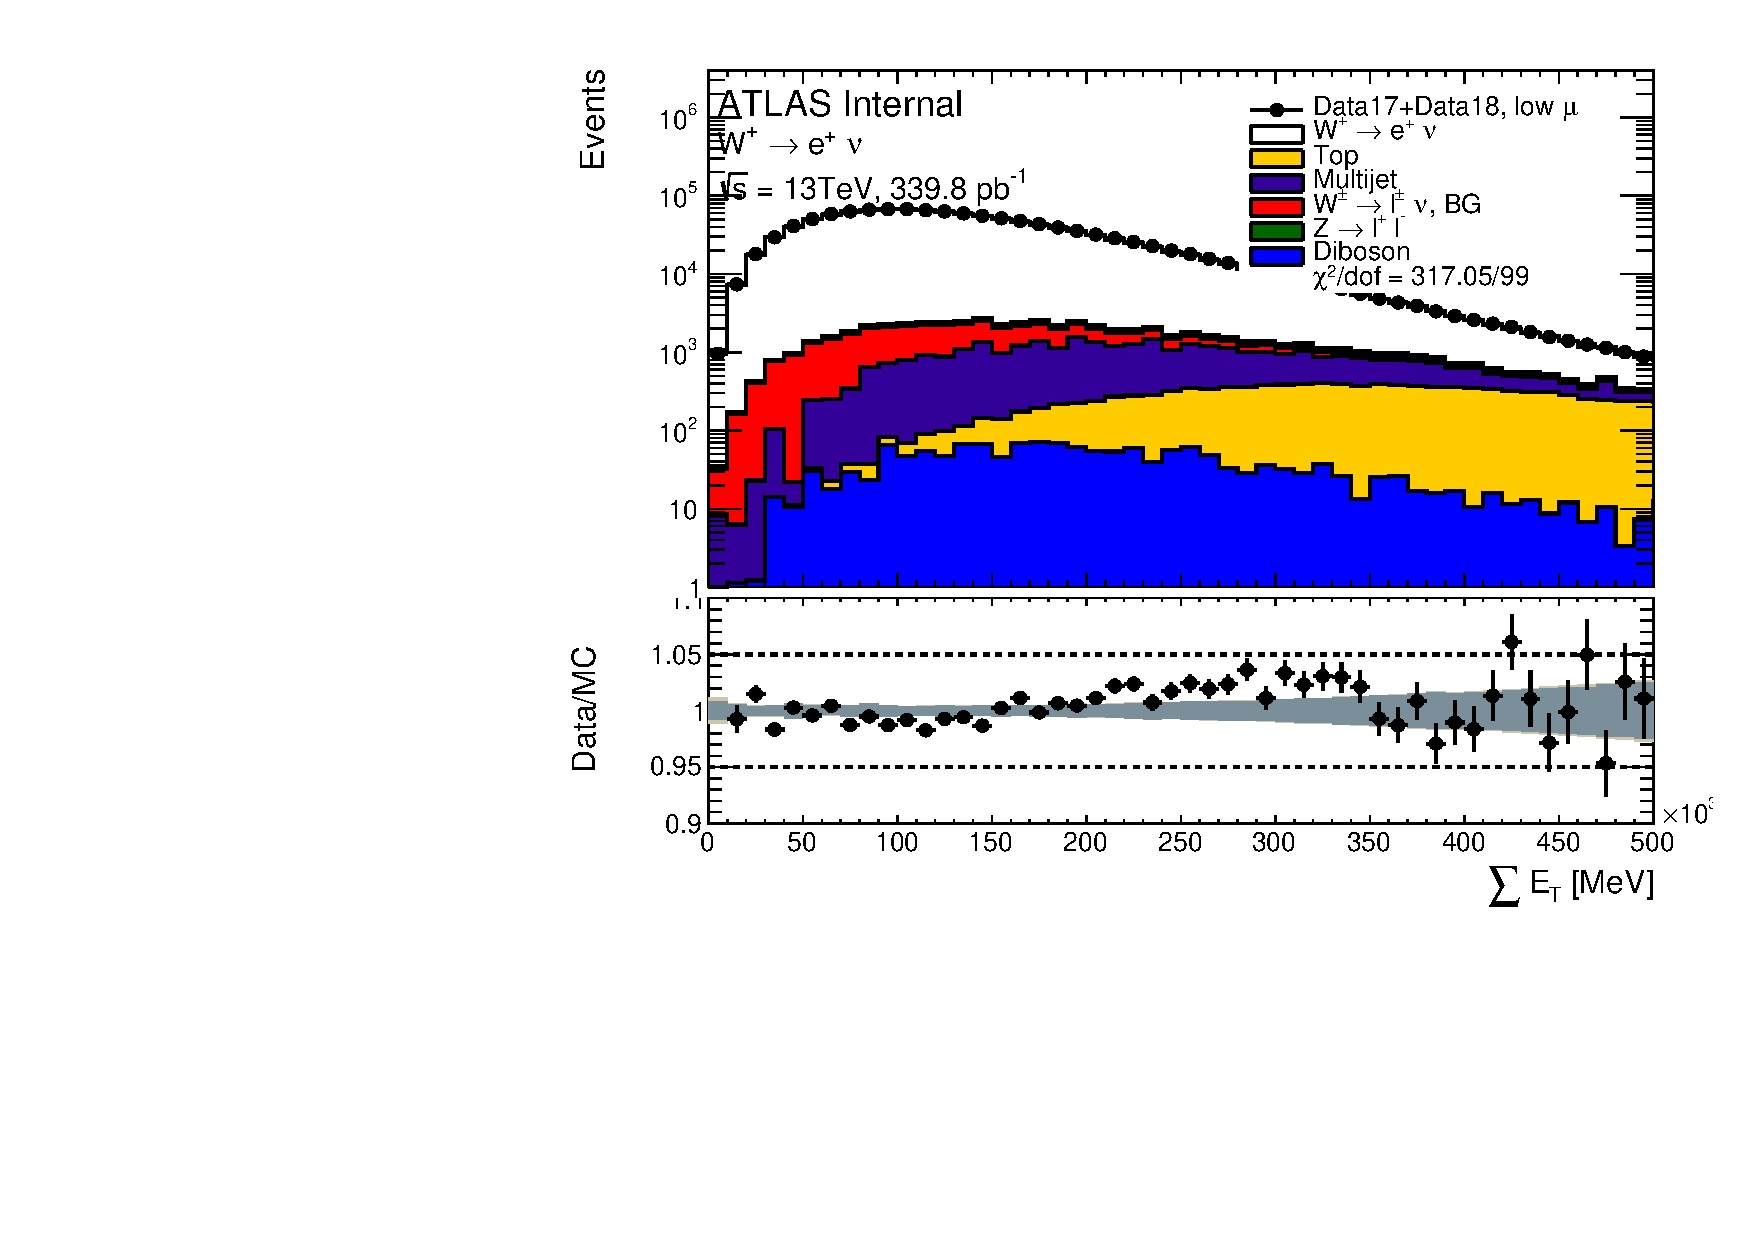
\includegraphics[width=.49\textwidth]{control_norm/SET_cut7_plusenu_13TeV_log_norm_NormErr.pdf}\label{f:}}
	\caption{$\Sigma{E_T}$ distribution in the muon and electron channel  for the $\sqrt{s} = 13$~\TeV\ dataset.}\end{figure}



\begin{figure}[h]
	\centering
	{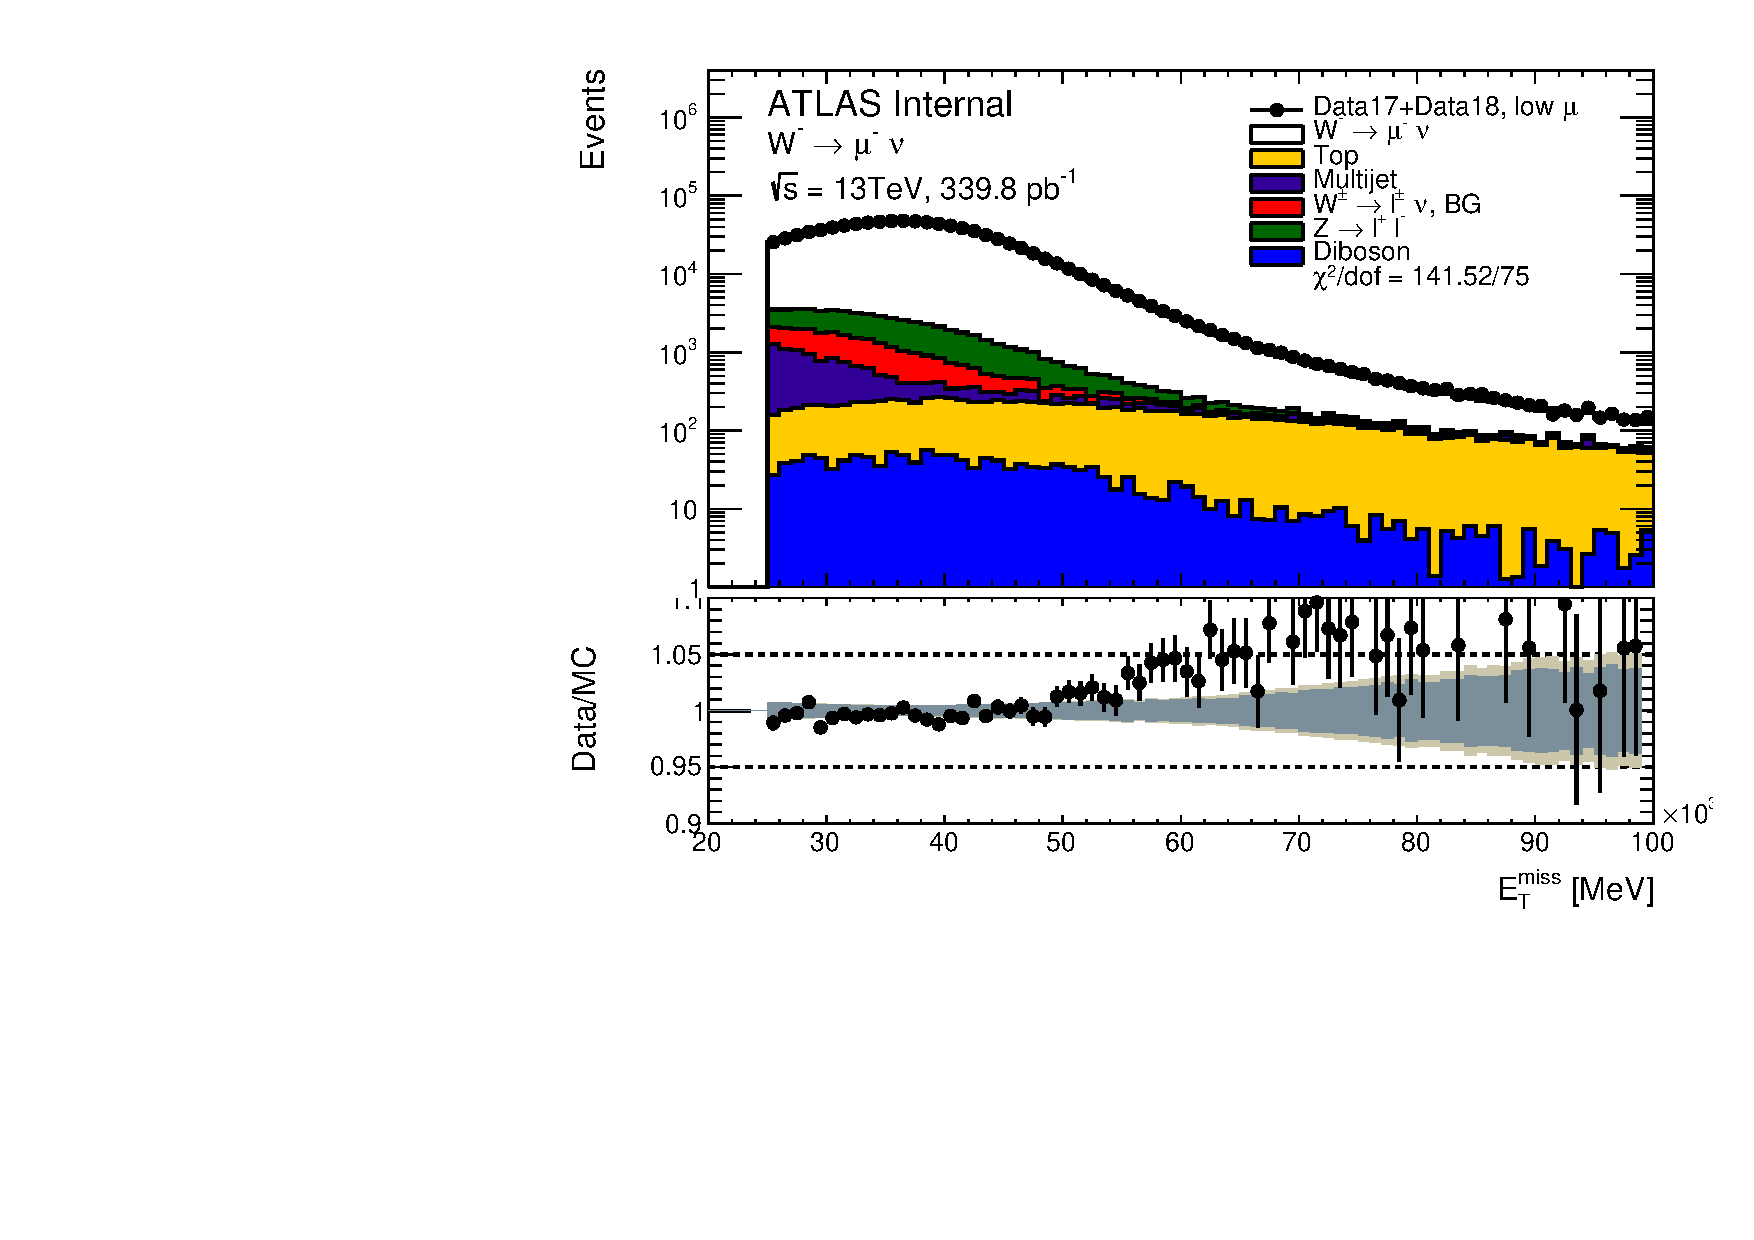
\includegraphics[width=.49\textwidth]{control_norm/met_cut7_minusmunu_13TeV_log_norm_NormErr.pdf}\label{f:}}
	{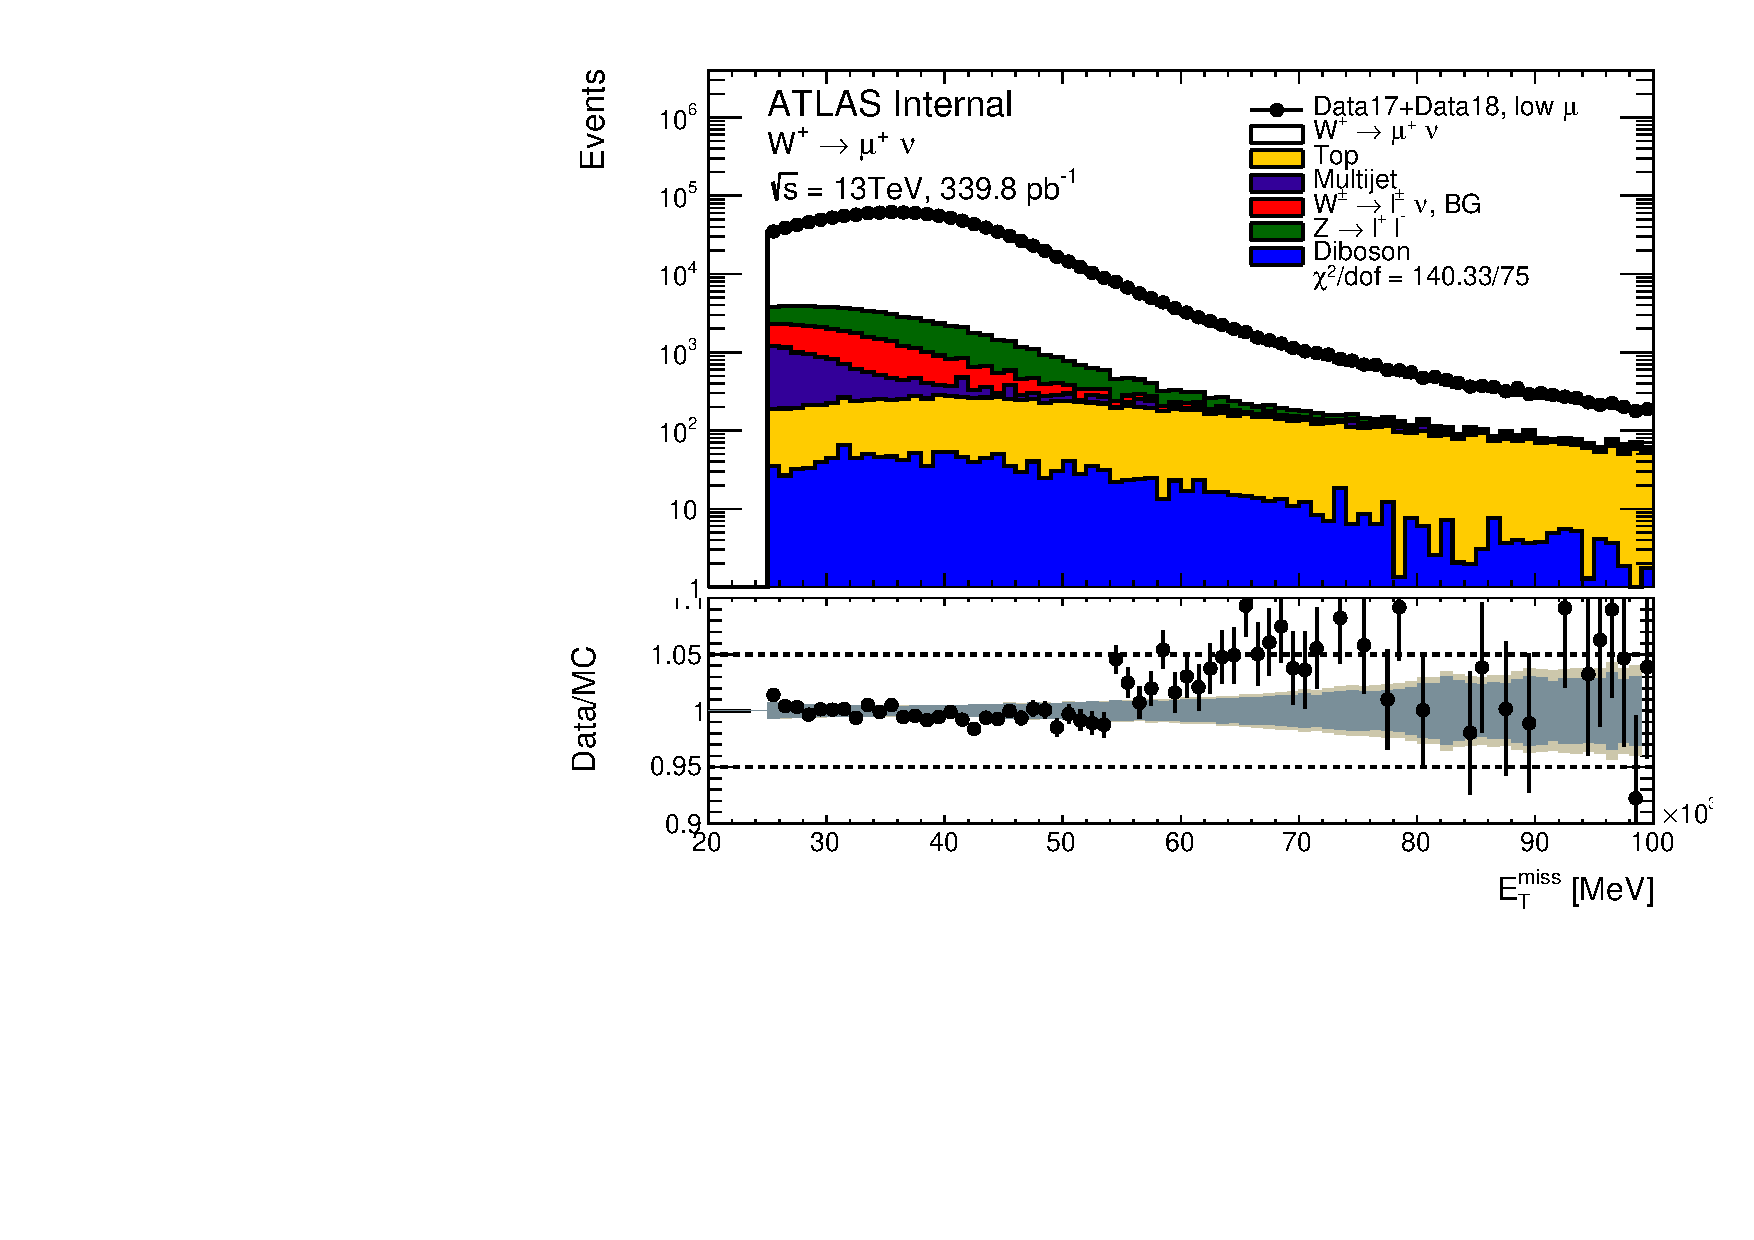
\includegraphics[width=.49\textwidth]{control_norm/met_cut7_plusmunu_13TeV_log_norm_NormErr.pdf}\label{f:}}
	
	{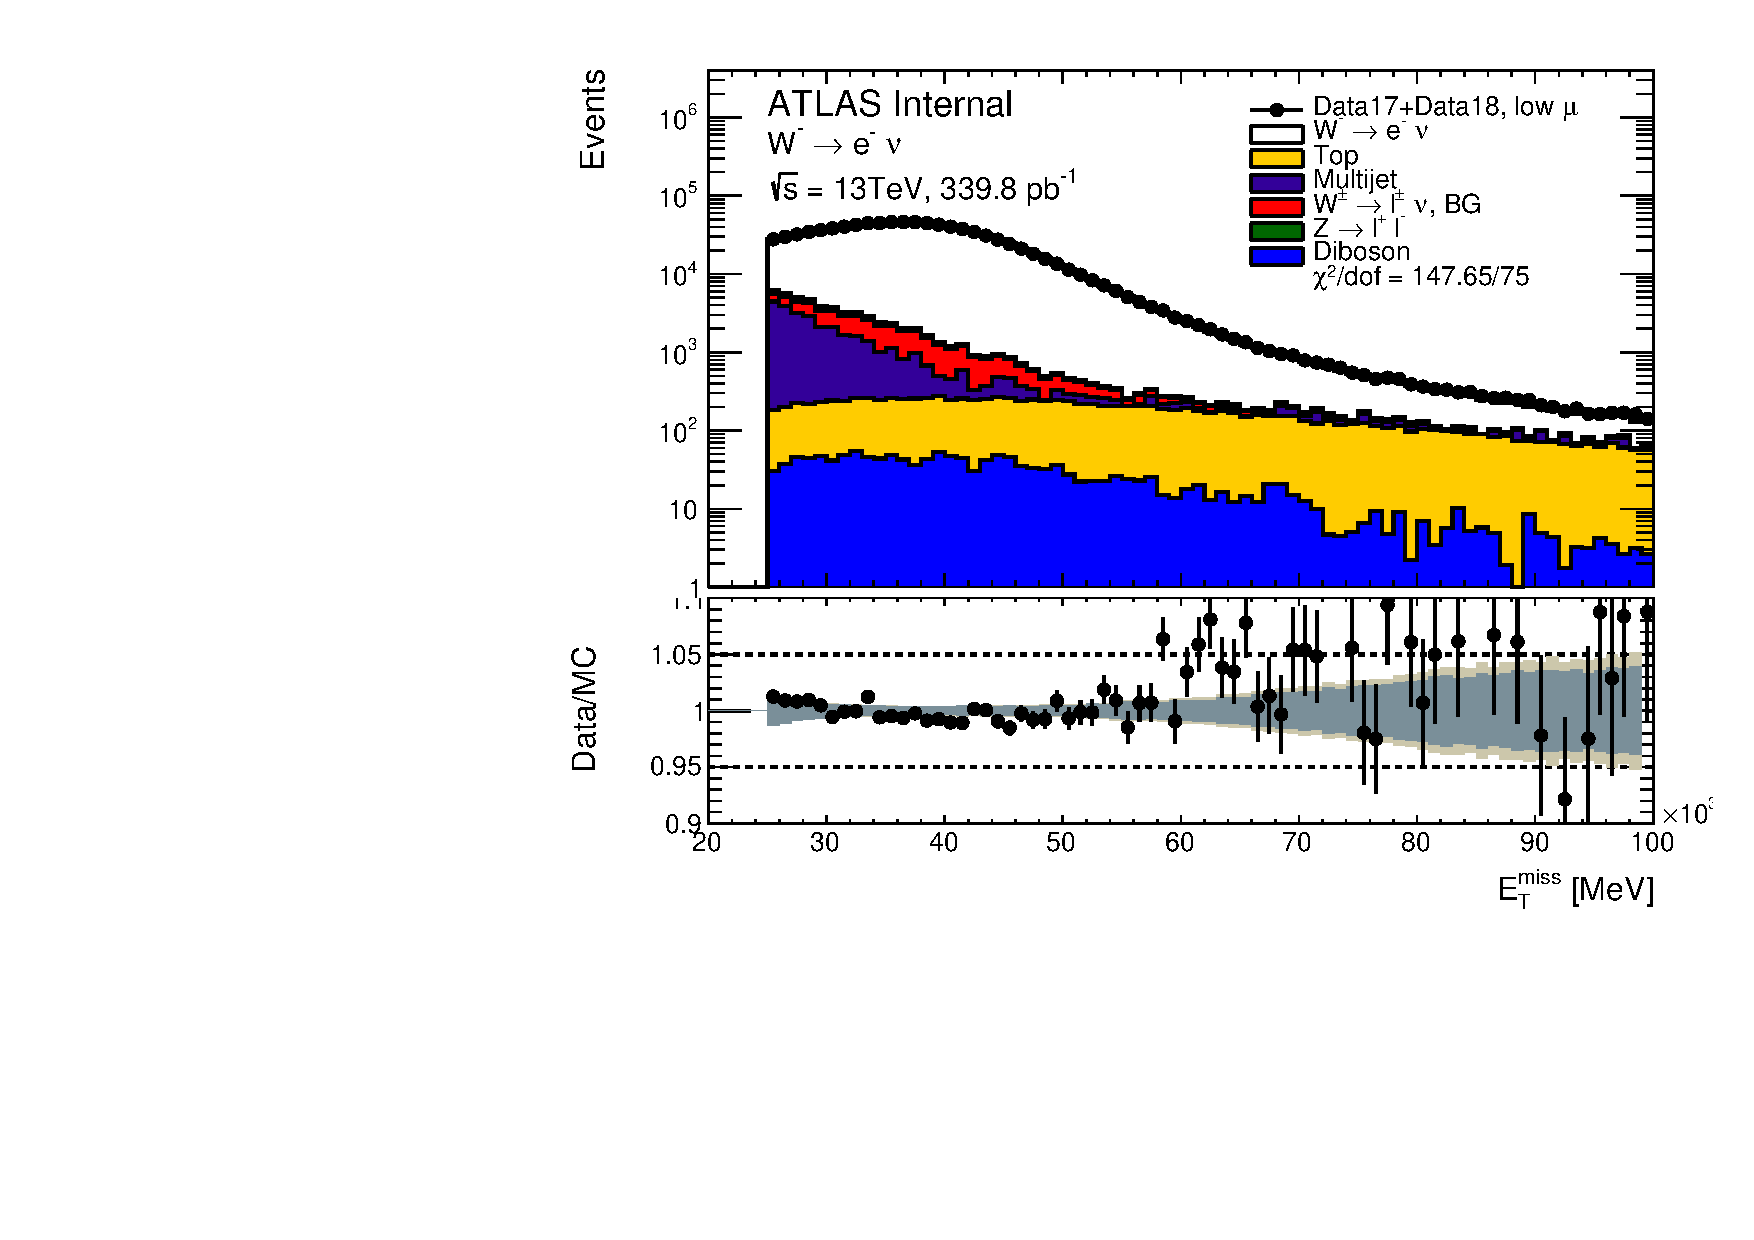
\includegraphics[width=.49\textwidth]{control_norm/met_cut7_minusenu_13TeV_log_norm_NormErr.pdf}\label{f:}}
	{\includegraphics[width=.49\textwidth]{control_norm/met_cut7_plusenu_13TeV_log_norm_NormErr.pdf}\label{f:}}
	\caption{ $\vec{E}^{miss}_{T}$ distribution in the muon and electron channel  for the $\sqrt{s} = 13$~\TeV\ dataset. }\end{figure}




\begin{figure}[h]
	\centering
	{\includegraphics[width=.49\textwidth]{control_norm/mT_cut7_minusmunu_13TeV_log_norm_NormErr.pdf}\label{f:}}
	{\includegraphics[width=.49\textwidth]{control_norm/mT_cut7_plusmunu_13TeV_log_norm_NormErr.pdf}\label{f:}}
	
	{\includegraphics[width=.49\textwidth]{control_norm/mT_cut7_minusenu_13TeV_log_norm_NormErr.pdf}\label{f:}}
	{\includegraphics[width=.49\textwidth]{control_norm/mT_cut7_plusenu_13TeV_log_norm_NormErr.pdf}\label{f:}}
	\caption{  Transverse mass distribution of the W boson in the muon and electron channel  for the $\sqrt{s} = 13$~\TeV\ dataset. }\end{figure}


\begin{figure}[h]
	\centering
	{\includegraphics[width=.49\textwidth]{control_norm/muEta_cut7_minusmunu_13TeV_log_norm_NormErr.pdf}\label{f:}}
	{\includegraphics[width=.49\textwidth]{control_norm/muEta_cut7_plusmunu_13TeV_log_norm_NormErr.pdf}\label{f:}}
	
	{\includegraphics[width=.49\textwidth]{control_norm/elEta_cut7_minusenu_13TeV_log_norm_NormErr.pdf}\label{f:}}
	{\includegraphics[width=.49\textwidth]{control_norm/elEta_cut7_plusenu_13TeV_log_norm_NormErr.pdf}\label{f:}}
	\caption{  Lepton pseudorapidity distribution in the muon and electron channel  for the $\sqrt{s} = 13$~\TeV\ dataset. }\end{figure}


\begin{figure}[h]
	\centering
	{\includegraphics[width=.49\textwidth]{control_norm/muPt_cut7_minusmunu_13TeV_log_norm_NormErr.pdf}\label{f:}}
	{\includegraphics[width=.49\textwidth]{control_norm/muPt_cut7_plusmunu_13TeV_log_norm_NormErr.pdf}\label{f:}}
	
	{\includegraphics[width=.49\textwidth]{control_norm/elPt_cut7_minusenu_13TeV_log_norm_NormErr.pdf}\label{f:}}
	{\includegraphics[width=.49\textwidth]{control_norm/elPt_cut7_plusenu_13TeV_log_norm_NormErr.pdf}\label{f:}}
	\caption{  Lepton transverse momentum distribution in the muon and electron channel  for the $\sqrt{s} = 13$~\TeV\ dataset. }\end{figure}



\begin{figure}[h]
	\centering
	{\includegraphics[width=.49\textwidth]{control_norm/WpT_Reco_cut7_minusmunu_13TeV_log_norm_NormErr.pdf}\label{f:}}
	{\includegraphics[width=.49\textwidth]{control_norm/WpT_Reco_cut7_plusmunu_13TeV_log_norm_NormErr.pdf}\label{f:}}
	
	{\includegraphics[width=.49\textwidth]{control_norm/WpT_Reco_cut7_minusenu_13TeV_log_norm_NormErr.pdf}\label{f:}}
	{\includegraphics[width=.49\textwidth]{control_norm/WpT_Reco_cut7_plusenu_13TeV_log_norm_NormErr.pdf}\label{f:}}
	\caption{  Hadronic recoil distribution in the muon and electron channel  for the $\sqrt{s} = 13$~\TeV\ dataset. }\end{figure}

%%%%% ************************* 5 TeV ****************************

\clearpage


\subsection{$\sqrt{s} = 5$~\TeV\ dataset control plots}
\label{subsec:controlplots5}
Control plots for the 5~\TeV\ \lowmu\ dataset are provided here after applying all corrections described in Section 7, and after applying the selection described above in this section. In each figure, the right(left)-hand column shows distributions for the \Wplus\ (\Wminus) process. The top (bottom) row shows the muon (electron) decay channel. In the ratio panels, the grey band is the total systematic uncertainty, whilst the brown band adds the MC statistical uncertainty in quadrature on top of it. In regions of the distributions insensitive to the modelling of \ptw\ there is generally good agreement between data and predictions. The bulk of the \mt\ distribution is a typical example of distribution that is mostly insensitive to the modeling of \ptw. Compared to the 13~\TeV\ situation, the \ut\ distribution seems to indicate that the baseline simulation models \ptw\ more satisfactorily.

\begin{figure}[h]
	\centering
	{\includegraphics[width=.49\textwidth]{control_norm/SETUE_cut7_minusmunu_5TeV_log_norm_NormErr.pdf}\label{f:SETUEmm5}}
	{\includegraphics[width=.49\textwidth]{control_norm/SETUE_cut7_plusmunu_5TeV_log_norm_NormErr.pdf}\label{f:SETUEpm5}}
	
	{\includegraphics[width=.49\textwidth]{control_norm/SETUE_cut7_minusenu_5TeV_log_norm_NormErr.pdf}\label{f:}}
	{\includegraphics[width=.49\textwidth]{control_norm/SETUE_cut7_plusenu_5TeV_log_norm_NormErr.pdf}\label{f:}}
	\caption{$\Sigma \bar{E_T}$ distribution in the muon and electron channel  for the $\sqrt{s} = 5$~\TeV\ dataset.}
\end{figure}
%

\begin{figure}[h]
	\centering
	{\includegraphics[width=.49\textwidth]{control_norm/SET_cut7_minusmunu_5TeV_log_norm_NormErr.pdf}\label{f:set5}}
	{\includegraphics[width=.49\textwidth]{control_norm/SET_cut7_plusmunu_5TeV_log_norm_NormErr.pdf}\label{f:setpl}}
	
	{\includegraphics[width=.49\textwidth]{control_norm/SET_cut7_minusenu_5TeV_log_norm_NormErr.pdf}\label{f:}}
	{\includegraphics[width=.49\textwidth]{control_norm/SET_cut7_plusenu_5TeV_log_norm_NormErr.pdf}\label{f:}}
	\caption{$\Sigma{E_T}$ distribution in the muon and electron channel  for the $\sqrt{s} = 5$~\TeV\ dataset.}
\end{figure}
\newpage


\begin{figure}[h]
	\centering
	{\includegraphics[width=.49\textwidth]{control_norm/met_cut7_minusmunu_5TeV_log_norm_NormErr.pdf}\label{f:}}
	{\includegraphics[width=.49\textwidth]{control_norm/met_cut7_plusmunu_5TeV_log_norm_NormErr.pdf}\label{f:}}
	
	{\includegraphics[width=.49\textwidth]{control_norm/met_cut7_minusenu_5TeV_log_norm_NormErr.pdf}\label{f:}}
	{\includegraphics[width=.49\textwidth]{control_norm/met_cut7_plusenu_5TeV_log_norm_NormErr.pdf}\label{f:}}
	\caption{ $\vec{E}^{miss}_{T}$ distribution in the muon and electron channel  for the $\sqrt{s} = 5$~\TeV\ dataset.}
\end{figure}
\newpage



\begin{figure}[h]
	\centering
	{\includegraphics[width=.49\textwidth]{control_norm/mT_cut7_minusmunu_5TeV_log_norm_NormErr.pdf}\label{f:}}
	{\includegraphics[width=.49\textwidth]{control_norm/mT_cut7_plusmunu_5TeV_log_norm_NormErr.pdf}\label{f:}}
	
	{\includegraphics[width=.49\textwidth]{control_norm/mT_cut7_minusenu_5TeV_log_norm_NormErr.pdf}\label{f:}}
	{\includegraphics[width=.49\textwidth]{control_norm/mT_cut7_plusenu_5TeV_log_norm_NormErr.pdf}\label{f:}}
	\caption{  Transverse mass distribution of the W boson in the muon and electron channel  for the $\sqrt{s} = 5$~\TeV\ dataset. }\end{figure}
\newpage

\begin{figure}[h]
	\centering
	{\includegraphics[width=.49\textwidth]{control_norm/muEta_cut7_minusmunu_5TeV_log_norm_NormErr.pdf}\label{f:}}
	{\includegraphics[width=.49\textwidth]{control_norm/muEta_cut7_plusmunu_5TeV_log_norm_NormErr.pdf}\label{f:}}
	
	{\includegraphics[width=.49\textwidth]{control_norm/elEta_cut7_minusenu_5TeV_log_norm_NormErr.pdf}\label{f:}}
	{\includegraphics[width=.49\textwidth]{control_norm/elEta_cut7_plusenu_5TeV_log_norm_NormErr.pdf}\label{f:}}
	\caption{  Lepton pseudorapidity distribution in the muon and electron channel  for the $\sqrt{s} = 5$~\TeV\ dataset. }\end{figure}
\newpage

\begin{figure}[h]
	\centering
	{\includegraphics[width=.49\textwidth]{control_norm/muPt_cut7_minusmunu_5TeV_log_norm_NormErr.pdf}\label{f:}}
	{\includegraphics[width=.49\textwidth]{control_norm/muPt_cut7_plusmunu_5TeV_log_norm_NormErr.pdf}\label{f:}}
	
	{\includegraphics[width=.49\textwidth]{control_norm/elPt_cut7_minusenu_5TeV_log_norm_NormErr.pdf}\label{f:}}
	{\includegraphics[width=.49\textwidth]{control_norm/elPt_cut7_plusenu_5TeV_log_norm_NormErr.pdf}\label{f:}}
	\caption{  Lepton transverse momentum distribution in the muon and electron channel  for the $\sqrt{s} = 5$~\TeV\ dataset. }\end{figure}
	\newpage
\begin{figure}[h]
	\centering
	{\includegraphics[width=.49\textwidth]{control_norm/WpT_Reco_cut7_minusmunu_5TeV_log_norm_NormErr.pdf}\label{f:}}
	{\includegraphics[width=.49\textwidth]{control_norm/WpT_Reco_cut7_plusmunu_5TeV_log_norm_NormErr.pdf}\label{f:}}

	{\includegraphics[width=.49\textwidth]{control_norm/WpT_Reco_cut7_minusenu_5TeV_log_norm_NormErr.pdf}\label{f:}}
	{\includegraphics[width=.49\textwidth]{control_norm/WpT_Reco_cut7_plusenu_5TeV_log_norm_NormErr.pdf}\label{f:}}
	\caption{  Hadronic recoil distribution in the muon and electron channel  for the $\sqrt{s} = 5$~\TeV\ dataset. }\end{figure}
	\newpage
	\clearpage
%
%

